\documentclass[]{report}
\usepackage{lmodern}
\usepackage{amssymb,amsmath}
\usepackage{ifxetex,ifluatex}
\usepackage{fixltx2e} % provides \textsubscript
\ifnum 0\ifxetex 1\fi\ifluatex 1\fi=0 % if pdftex
  \usepackage[T1]{fontenc}
  \usepackage[utf8]{inputenc}
\else % if luatex or xelatex
  \ifxetex
    \usepackage{mathspec}
  \else
    \usepackage{fontspec}
  \fi
  \defaultfontfeatures{Ligatures=TeX,Scale=MatchLowercase}
\fi
% use upquote if available, for straight quotes in verbatim environments
\IfFileExists{upquote.sty}{\usepackage{upquote}}{}
% use microtype if available
\IfFileExists{microtype.sty}{%
\usepackage{microtype}
\UseMicrotypeSet[protrusion]{basicmath} % disable protrusion for tt fonts
}{}
\usepackage[unicode=true]{hyperref}
\PassOptionsToPackage{usenames,dvipsnames}{color} % color is loaded by hyperref
\hypersetup{
            pdftitle={Os Maiores Litigantes da Justiça Consumerista: Mapeamento e Proposições},
            pdfauthor={Associação Brasileira de Jurimetria},
            colorlinks=true,
            linkcolor=Maroon,
            citecolor=Blue,
            urlcolor=Blue,
            breaklinks=true}
\urlstyle{same}  % don't use monospace font for urls
\usepackage{natbib}
\bibliographystyle{apalike}
\usepackage{longtable,booktabs}
\usepackage{graphicx,grffile}
\makeatletter
\def\maxwidth{\ifdim\Gin@nat@width>\linewidth\linewidth\else\Gin@nat@width\fi}
\def\maxheight{\ifdim\Gin@nat@height>\textheight\textheight\else\Gin@nat@height\fi}
\makeatother
% Scale images if necessary, so that they will not overflow the page
% margins by default, and it is still possible to overwrite the defaults
% using explicit options in \includegraphics[width, height, ...]{}
\setkeys{Gin}{width=\maxwidth,height=\maxheight,keepaspectratio}
\IfFileExists{parskip.sty}{%
\usepackage{parskip}
}{% else
\setlength{\parindent}{0pt}
\setlength{\parskip}{6pt plus 2pt minus 1pt}
}
\setlength{\emergencystretch}{3em}  % prevent overfull lines
\providecommand{\tightlist}{%
  \setlength{\itemsep}{0pt}\setlength{\parskip}{0pt}}
\setcounter{secnumdepth}{5}
% Redefines (sub)paragraphs to behave more like sections
\ifx\paragraph\undefined\else
\let\oldparagraph\paragraph
\renewcommand{\paragraph}[1]{\oldparagraph{#1}\mbox{}}
\fi
\ifx\subparagraph\undefined\else
\let\oldsubparagraph\subparagraph
\renewcommand{\subparagraph}[1]{\oldsubparagraph{#1}\mbox{}}
\fi
\usepackage[brazilian]{babel}
\usepackage[utf8]{inputenc}
\usepackage[T1]{fontenc}
\usepackage{lipsum}
\usepackage{fullwidth}
\usepackage{indentfirst}
\usepackage[left=2.5cm, right=2.5cm, top=4cm, bottom=3.8cm]{geometry}
\renewcommand{\familydefault}{\sfdefault}
\PassOptionsToPackage{dvipsnames}{xcolor}
\RequirePackage{xcolor} % [dvipsnames]
\definecolor{halfgray}{gray}{0.55} % chapter numbers will be semi transparent .5 .55 .6 .0
\definecolor{webgreen}{rgb}{0,.5,0}
\definecolor{webbrown}{rgb}{.6,0,0}
%\definecolor{Maroon}{cmyk}{0, 0.87, 0.68, 0.32}
%\definecolor{RoyalBlue}{cmyk}{1, 0.50, 0, 0}
%\definecolor{Black}{cmyk}{0, 0, 0, 0}
\usepackage{fancyhdr}
\usepackage{pdfpages}
\usepackage{amsmath}
\usepackage{graphicx}
\usepackage{listings}
\usepackage{enumitem}
\usepackage{setspace}
\usepackage{spverbatim}
\usepackage{lipsum}
\usepackage{natbib}
\usepackage{longtable}
\usepackage{booktabs}
\usepackage{background}

\renewcommand{\baselinestretch}{1.4}
\newcommand{\prestadorEmpresaFoot}{Associação Brasileira de Jurimetria}
\newcommand{\prestadorEmpresa}{Associação Brasileira de Jurimetria}
\newcommand{\prestadorRepr}{Marcelo Guedes Nunes}
\newcommand{\prestadorEnderecoFoot}{Rua Gomes de Carvalho, 1356, 2º andar. CEP 04547-005 - São Paulo, SP, Brasil.}
\newcommand{\prestadorEndereco}{Rua Gomes de Carvalho, 1356, 2º andar}
\newcommand{\prestadorEnderecoComp}{CEP 04547-005 - São Paulo, SP, Brasil}
\newcommand{\prestadorSite}{\url{http://abj.org.br}}
\newcommand{\prestadorEmail}{contato@abj.org.br}
% \includegraphics[trim=left bottom right top, clip]{file}
\newcommand{\logo}{
\includegraphics[width=0.21\textwidth, trim=0cm 0cm 0cm 11.1cm, clip]{logo_abj_final_2.png}}

\newcommand{\tipoTrabalho}{}
\newcommand{\numero}{XXX}

\newcommand{\clienteEmpresa}{XXX}
\newcommand{\clienteEndereco}{XXX}
\newcommand{\clienteEnderecoComp}{XXX}
\newcommand{\clienteRepr}{XXX}
\newcommand{\clienteEmail}{XXX}

% \fancypagestyle{firststyle}
% {
%     \pagestyle{fancy}
%     \lhead{\thepage}
%     \chead{}
%     \rhead{\logo{}}
%     \cfoot{
%         \footnotesize{\prestadorEmpresaFoot{}} \\
%         \footnotesize{\prestadorEnderecoFoot{}} \\
%         \footnotesize{\prestadorSite{}}
%     }
%     \renewcommand{\headrulewidth}{0.5pt}
%     \renewcommand{\footrulewidth}{0.5pt}
%     \setlength{\headsep}{.5in}
% }
%
% \pagestyle{firststyle}

\setlength{\parindent}{2em}
% \setlength{\parskip}{1em}
% \renewcommand{\baselinestretch}{1.2}
% % \usepackage{palatino}
% \renewcommand{\familydefault}{\sfdefault} % sans serif
% \fontfamily{ppl}\selectfont

%\renewcommand{\baselinestretch}{1.4}

\backgroundsetup{
scale=1,
angle=0,
opacity=1,
color=black,
contents={\begin{tikzpicture}[remember picture,overlay]
\node at ([xshift=-4.35cm,yshift=-2.5cm] current page.north east) % Adjust the position of the logo.
{
\includegraphics[width=0.21\textwidth, trim=0cm 0cm 0cm 11.1cm, clip]{logo_abj_final_2.png}}; % logo goes here
\end{tikzpicture}}
}

\title{Os Maiores Litigantes da Justiça Consumerista: Mapeamento e Proposições}
\author{Associação Brasileira de Jurimetria}
\date{01 de setembro de 2017}

\begin{document}
\maketitle

{
\hypersetup{linkcolor=black}
\setcounter{tocdepth}{2}
\tableofcontents
}
\listoftables
\listoffigures
\chapter{Introdução}\label{introducao}

Estudos recentes indicam que ações envolvendo o direito do consumidor
têm grande influência no volume de processos no Poder Judiciário.
Somente em 2014, foram mais de dois milhões de casos novos envolvendo
responsabilidade do fornecedor ou indenização por dano moral, situando o
assunto como o terceiro mais demandado de todos os tribunais, com pelo
menos 4\% de todas as novas demandas do ano de 2014 \citep{CNJ2015}.

Diante desse cenário, compreender o volume e o perfil dos processos que
envolvem direito do consumidor é condição necessária para uma boa
administração da Justiça. Em relação ao volume, para a mensuração do
impacto desses processos na taxa de congestionamento dos tribunais, é
preciso levantar não só os casos novos mas também o estoque e o tempo de
duração médio dos processos. Já em relação ao perfil, precisamos
entender como se distribuem os processos no tempo e no espaço, quem são
os maiores responsáveis pela litigiosidade e quais as principais
características dos processos. Somente com essas informações é possível
planejar e implementar políticas públicas e mudanças legislativas de
qualidade.

Ainda sobre o perfil dos processos, uma hipótese recorrente no direito
do consumidor é de que um pequeno grupo de litigantes são réus na maior
parte dos processos judiciais. O estudo ``100 maiores litigantes''
\citep{CNJ2012} mostra, por exemplo, que na 1ª instância da Justiça
Estadual, os cem maiores litigantes figuram como uma das partes em 36\%
dos processos. Na justiça consumerista, espera-se que essa proporção
seja ainda maior.

Supondo que a hipótese supracitada seja válida, podemos reduzir o
universo de investigação somente para os processos envolvendo os maiores
litigantes. Essa simplificação é coerente por dois motivos:
primeiramente, se compreendermos e solucionarmos os problemas envolvendo
os maiores litigantes, teremos atingido uma parte considerável do volume
total de processos, o que já é suficiente para o desenvolvimento e
implementação de políticas públicas. Além disso, ao estudar somente os
processos envolvendo um conjunto fixado de litigantes, controlamos a
incerteza e possibilitamos estudos mais aprofundados do tema, aumentando
as chances de se obter resultados úteis e propositivos.

A presente pesquisa teve como hipótese primordial a de que trinta
litigantes estavam envolvidos como réus em uma proporção relevante das
ações consumeristas em tramitação na justiça estadual. A hipótese foi
verificada a partir das extrações de dados dos tribunais, considerando
diferentes cortes de tempo, região e perfil empresarial.

Em seguida, partimos para uma investigação mais aprofundada e
propositiva sobre seis temas específicos, cada um associado a uma faceta
do problema e uma ou mais recomendações para sua solução. Os temas foram
agrupados em duas perguntas principais: a) ``o que fazer com o estoque
atual de processos?'' e b) ``como evitar a entrada de tantos
processos?''.

Nesse trabalho, descrevemos a metodologia para obtenção dos maiores
litigantes e mostramos os principais resultados da pesquisa. No final,
apresentamos sugestões para a melhoria da administração
judiciária.

\section{Justificativa}\label{justificativa}

A justiça brasileira possui hoje substanciais repositórios de processos
judiciais. Os montantes são do conhecimento do setor e dos diversos
segmentos da sociedade, assim como os prazos decorridos até a decisão
final tramitada em julgado. Esses volumes são significativos e mais
ainda são os valores envolvidos.

De modo geral, a ausência de bancos de dados adequadamente projetados,
sem redundâncias ou inconsistências e de análises estatísticas robustas,
parece levar a uma situação de grande dificuldade para a administração
da justiça e, em consequência, a uma limitação dos recursos
orçamentários disponíveis para custeio e investimento.

Nos últimos anos, o CNJ vem desenvolvendo um esforço hercúleo nesse
sentido. Graças a iniciativas como o Justiça em Números e projetos de
pesquisa aplicados a determinados segmentos da Justiça, já é possível
obter visões gerais do funcionamento do Judiciário e identificar alguns
de seus principais gargalos. No entanto, os trabalhos ainda estão
adquirindo maturidade e, por isso, não proporcionam resultados definitivos
frente a perguntas como ``por quê temos tantos processos?'', de modo que
há dificuldades em elaborar políticas públicas adequadas para resolver
problemas importantes como reduzir o volume de ações.

Nesse cenário surge a necessidade de desenvolvimento de um projeto que
auxilie a equacionar uma das restrições colocadas: bases de dados e
modelos estatísticos de análise de processos, com as respectivas
métricas de resultados, possibilitando um melhor conhecimento das ações
por setor litigante, partes envolvidas e causas de pedir. O
propósito é de que os resultados obtidos nos estudos aumentem o
entendimento que o Poder Judiciário tem a respeito de novos litígios e
sirva de fundamento para o desenvolvimento de ações pontuais
estratégicas que permitam solucionar gargalos já existentes e prevenir
um volume exagerado de novos litígios.

O presente tema é uma oportunidade da ABJ de disseminar o conceito, as
metodologias e as aplicações da jurimetria, a fim de introduzir e
disciplinar o rigor no planejamento, amostragem e análise estatística de
dados jurídicos, e trazer, como consequência, um relatório verossímil e
funcional para a utilização do CNJ para elaboração de políticas
públicas.

\section{Levantamento Bibliográfico}\label{levantamento-bibliografico}

O estudo ``100 maiores litigantes'' \citep{CNJ2012}, divulgado pelo
Departamento de Pesquisas Judiciárias é o primeiro estudo sistemático
realizado sobre maiores litigantes e teve impacto profundo na comunidade
jurídica. O estudo indica que uma parcela considerável do volume
processual pode ser atribuída aos cem maiores litigantes. Por exemplo,
na 1ª instância da Justiça Estadual, esses litigantes figuram como uma
das partes em 36\% do volume processual.

O estudo ``O uso da justiça e o litígio no Brasil'' \citep{AMB2015}
sugere que a maior parte dos processos está associada aos setores
financeiro e de telefonia. O trabalho também defende a importância da
realização de estudos aprofundados sobre litígios em massa e técnicas de
solução de conflitos, como conciliação e mediação.

Por conta da alta concentração do volume processual em um pequeno
conjunto de réus, a atenção doutrinária voltou-se à litigância
repetitiva \citep{Silva2012}. A motivação é a de que alterações nessa
área podem trazer enormes ganhos à celeridade da Justiça.

Um tipo de alteração envolve modificações que facilitem a formação de
ações coletivas e litisconsórcios \citep[Marquezini2013,
Souza2014]{Mollica2010}. Agrupar sob uma única ação processos
semelhantes pode levar a uma melhor divisão do trabalho entre
magistrados, tornando mais célere a resolução dos conflitos. Tal
agrupamento também pode permitir ao magistrado definir grupos de
litigantes factualmente semelhantes e, assim, determinar compensações
com base em amostragem estatística \citep{Weinstein1997}.

Outro tipo de alteração envolve evitar que as causas ajuizadas contra os
maiores litigantes cheguem à Justiça. Um dos meios propostos é o
incentivo à resolução de conflitos por meio de arbitragem e mediação
\citep{Asperti2014}. Outro meio proposto é a revogação de leis que
obriguem o procurador público derrotado em primeira instância a recorrer
da decisão, independentemente dos seus prospectos de sucesso.

Uma terceira forma de abordar o tema da litigância repetitiva é através
do \emph{Incidente de Resolução de Demandas Repetitivas} (IRDR),
definido no novo Código Processual Civil (CPC), de 2015. O IRDR é
cabível quando houver, simultaneamente, duas condições: i) efetiva
repetição de processos que contenham controvérsia sobre a mesma questão
unicamente de direito, tanto material quanto processual; e ii) risco de
ofensa à isonomia e à segurança jurídica. No entanto, como a aplicação
do IRDR ainda é limitada, não existem estudos aprofundados que
investiguem quantitativamente o efeito do IRDR na taxa de
congestionamento do judiciário, especialmente no que se refere ao
direito do consumidor.

Uma forma mais abstrata de investigar o tema envolve modificações na lei
que visem criar incentivos econômicos para que as partes não ingressem
com ações judiciais. Por um lado, estudos como \citep{Athos2015}
investigam a possibilidade de existir uma ``indústria do dano moral'',
com base na inexistência das custas processuais e sucumbência nos
Juizados Especiais Cíveis (JEC). Por uma análise econômica, os autores
concluem que a inexistência de custas nos JEC poderia incentivar as
partes a sempre ingressarem com ações, mesmo quando a probabilidade de
sucesso é baixa.

De perspectiva diferente, também pode-se estudar empresas como agentes
maximizadores de lucro. Sob essa ótica, uma empresa escolheria
desrespeitar a lei, quando essa escolha traz maiores prospectos de
lucro. Esse tipo de análise traz à tona quais normas poderiam ser
criadas pelo Estado ou agências reguladoras de tal forma a tornar a
solução economicamente vantajosa para as empresas sem desrespeitar os
direitos do consumidor.

Os estudos evidenciaram a existência de dois grandes focos de
investigação. No primeiro, propomos mudanças administrativas e
legislativas para redução eficaz do estoque atual de processos. Já no
segundo, procuramos realizar ações preventivas e modificar incentivos
para litigar, buscando reduzir o volume de casos novos.

Dentro do primeiro foco, o tema mais discutido tratou da composição
amigável no processo através do incentivo à conciliação. O segundo tema
mais desenvolvido foi a litigância repetitiva, principalmente
relacionando o tema com o novo CPC. 

No segundo foco, as ideias são esparsas e é difícil elencar uma que se
sobressai perante as demais. Podemos elencar como eixos mais
importantes: i) o estudo dos incentivos para litigar, tanto do ponto de
vista do consumidor quanto da empresa; ii) mecanismos de composição
extrajudicial de conflitos, como mediação e ferramentas de comunicação
entre as partes (Reclame Aqui e Consumidor.gov.br, entre outros); e iii)
meios de agrupamento de conflitos em ações coletivas e litisconsórcios.

\section{Objetivos}\label{objetivos}

Os objetivos da presente pesquisa são:

\begin{enumerate}
\def\labelenumi{\arabic{enumi}.}
\tightlist
\item
  Levantar os maiores litigantes em ações consumeristas na Justiça
  Estadual.
\item
  Estudar as características dos litigantes e de seus litígios.
\item
  Avaliar de que forma os maiores litigantes variam regionalmente.
\item
  Estudar as características dos meios alternativos ao litígio.
\item
  Investigar como as grandes empresas do setor privado veem o problema
  das ações consumeristas.
\item
  Propor soluções administrativas para lidar com os casos pendentes e
  reduzir a entrada de novos casos no judiciário.
\end{enumerate}

\section{Hipóteses}\label{hipoteses}

As hipóteses de pesquisa definem o conjunto mínimo de investigações a
serem realizadas para atendimento dos objetivos específicos. Nesse
projeto, a principal hipótese avaliada (e trabalhada no capítulo
\protect\hyperlink{metodologia}{metodologia}) é a de que os trinta
maiores litigantes, em âmbito global, concentram uma proporção elevada
do total de ações consumeristas na Justiça Estadual. Chamamos essa parte
da pesquisa de \emph{exploratória}. A partir dela, emergiram outras
hipóteses e investigações.

Com o intuito de sistematizar o nosso estudo e deixá-lo mais próximo da
elaboração de políticas públicas, também trabalhamos com hipóteses
relacionadas ao que chamamos de parte \emph{propositiva} da pesquisa:

\begin{enumerate}
\def\labelenumi{\arabic{enumi}.}
\tightlist
\item
  O que pode ser feito para agilizar a tramitação dos processos
  consumeristas e reduzir o estoque de processos?

  \begin{enumerate}
  \def\labelenumii{\arabic{enumii}.}
  \tightlist
  \item
    Qual é o impacto da utilização de estratégias de composição
    amigável?
  \item
    O uso dos incidentes de demandas repetitivas do novo Código do
    Processo Civil pode ser efetivo na redução do número de processo em
    curso?
  \item
    É possível tornar o trabalho de uma vara mais eficiente utilizando
    alguma estratégia de ordenação da sua fila de processos?
  \end{enumerate}
\item
  O que pode diminuir o número de processos consumeristas que entram no
  judiciário?

  \begin{enumerate}
  \def\labelenumii{\arabic{enumii}.}
  \tightlist
  \item
    O brasileiro costuma buscar meios alternativos para a solução de
    conflitos antes de entrar com ações judiciais? Tais meios são
    efetivos?
  \item
    Existem fatores que incentivam o cometimento de ilícitos por parte
    das empresas? (Vantagem monetária, falta de regulamentação etc.)
  \item
    Existem fatores que incentivam a litigância excessiva dos
    consumidores? (indústria do dano moral, gratuidade judiciária etc.)
  \end{enumerate}
\end{enumerate}

Cada questão norteadora descrita acima deu origem a um eixo de
investigação, subtópicos do tema principal da pesquisa relacionados à
tramitação dos processos dos maiores litigantes da justiça consumerista.
Os eixos de investigação foram discutidos em detalhe no capítulo 
\protect\hyperlink{metodologia}{metodologia} e nos Apêndices.

\section{Resultados Esperados}\label{resultados-esperados}

Os resultados esperados dessa pesquisa foram:

\begin{enumerate}
\def\labelenumi{\arabic{enumi}.}
\tightlist
\item
  Tabelas e gráficos envolvendo os trinta maiores litigantes na Justiça
  Consumerista em sete Unidades Federativas (UFs).
\item
  Avanços metodológicos quantitativos, reprodutíveis e de código aberto,
  para tratamento de assuntos processuais e nomes de empresas.
\item
  Apresentação de uma lista de sugestões para aprimoramento da
  administração do judiciário.
\end{enumerate}

\section{Organização do trabalho}\label{organizacao-do-trabalho}

O produto final da pesquisa está organizado em três capítulos, além
dessa introdução. O capítulo
\protect\hyperlink{metodologia}{metodologia} descreve a metodologia
empregada na pesquisa. O capítulo
\protect\hyperlink{resultados}{resultados} mostra os principais
resultados. O capítulo
\protect\hyperlink{sugestoes-para-aprimoramento-do-sistema}{sugestoes-para-aprimoramento-do-sistema}
lista sugestões para o aprimoramento do sistema.

\hypertarget{metodologia}{\chapter{Metodologia}\label{metodologia}}

Na introdução vimos que a pesquisa apresenta uma parte
\emph{exploratória} e uma parte \emph{propositiva}. A primeira envolve o
levantamento dos maiores litigantes em ações consumeristas e a segunda
envolve propor soluções para lidar com o estoque de processos atual e
evitar novos casos. Nesse capítulo, descrevemos a metodologia utilizada
para solucionar os problemas de cada parte.

A pesquisa foi conduzida com base filosófica pragmática
\citep{hanson2005mixed}. Isso significa que o foco principal são
resultados aplicáveis à sociedade. O rigor metodológico reside
principalmente na parte exploratória, especificamente nos métodos
estatísticos de análise e inferência.

A pesquisa também buscou atender o \emph{princípio da reprodutibilidade}
\citep{gelman2014bayesian}. Com isso será possível utilizar o material
desenvolvido em outros trabalhos, produzindo um efeito maior do que
apenas a documentação de resultados.

A metodologia do estudo considerou um desenho misto
(\citet{hanson2005mixed}, p.~116). Especificamente, utilizamos a técnica
de métodos convergentes em paralelo (\emph{convergent parallel methods
design}). Nessa abordagem, coletamos e analisamos dados qualitativos e
quantitativos em paralelo, confrontando os resultados para gerar
interpretações e conclusões. A Figura \ref{fig:desenho} mostra
esquematicamente o desenho utilizado.

A parte exploratória utilizou métodos quantitativos baseados em dados
observacionais para elucidar o fenômeno de interesse
(\citet{hanson2005mixed}, p.~18). Nesse caso, iniciamos com a obtenção
de dados para posterior análise e interpretação de resultados. A Figura
\ref{fig:quanti} mostra essa parte de forma esquemática.

\begin{figure}[!htbp]
\centering
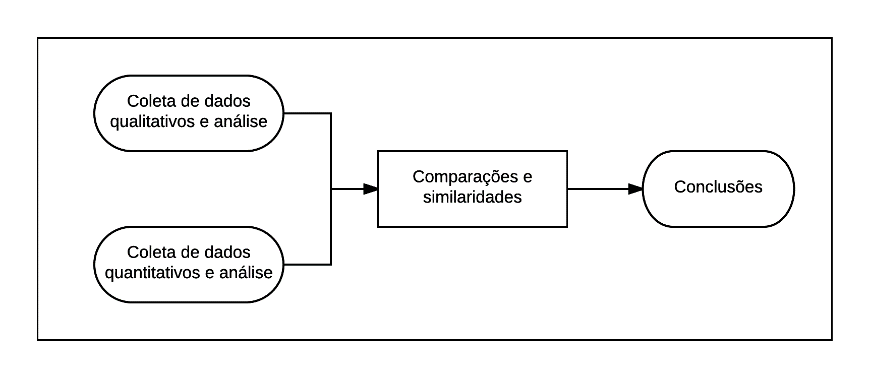
\includegraphics{imgs/creswell.png}
\caption{Método misto em paralelo convergente (adaptado de
\citep{creswell2013research}, p.~270).}\label{fig:desenho}
\end{figure}

Já a parte propositiva utilizou tanto métodos quantitativos
não-experimentais quanto métodos qualitativos para gerar as proposições.
Nesse caso, fizemos entrevistas, levantamentos bibliográficos e
levantamento de dados para suportar as argumentações.

\begin{figure}[!htbp]
\centering
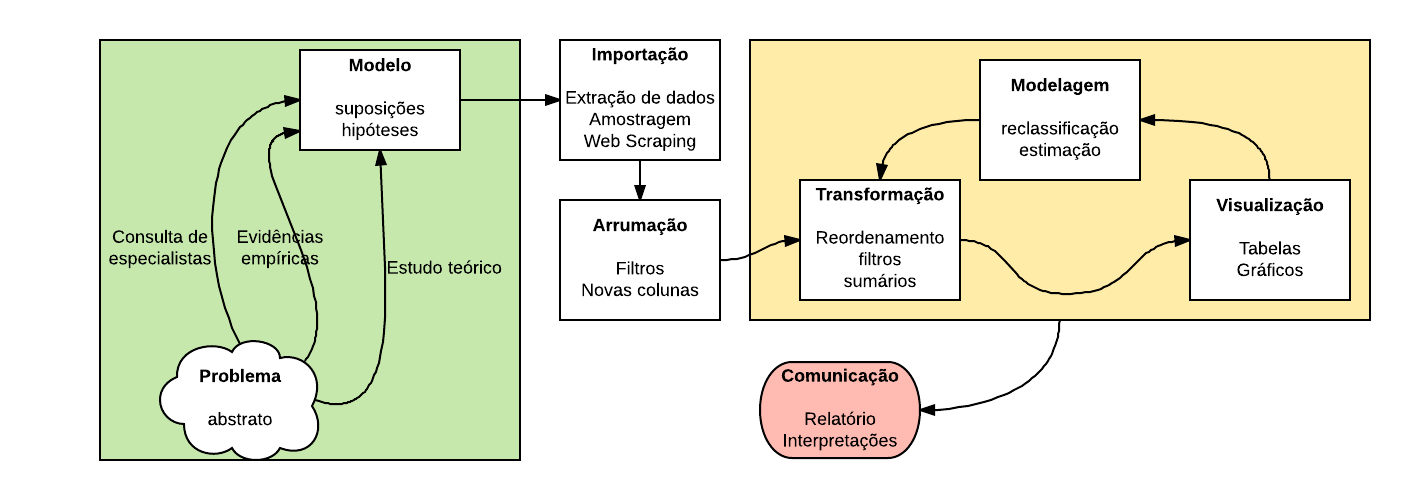
\includegraphics{imgs/quanti.png}
\caption{Metodologia quantitativa. Adaptado de
\citet{wickham2016r}.}\label{fig:quanti}
\end{figure}

A convergência das duas partes da pesquisa se deu a partir do
confrontamento dos resultados levantados (\citet{creswell2013research},
p.118). Os resultados da parte exploratória são utilizados como
\emph{inputs} para tomadas de decisão na parte propositiva, com o
intuito de i) descartar parte das proposições ou ii) indicar formas de
execução das propostas focadas em grupos estratégicos identificados na
parte exploratória (e.g.~regiões ou tipos empresariais).

A seguir, descrevemos a metodologia em maior detalhe. A Seção
\ref{parte-exploratoria} contempla os métodos de obtenção e análise dos
dados. A Seção \ref{parte-propositiva} descreve as atividades realizadas
da parte propositiva.

\section{Parte exploratória}\label{parte-exploratoria}

Nessa parte da metodologia, utilizamos dados e informações de outras
pesquisas para resolver algumas questões de escopo e direcionamento da
pesquisa. Especificamente, trabalhamos i) a direção da pesquisa; ii) a
situação atual; iii) a execução dos trabalhos; iv) a validação dos
resultados.

Os resultados dessas investigações foram resumidos abaixo. Em seguida,
apresentamos uma subseção de detalhamento para cada item.

\begin{enumerate}
\def\labelenumi{\arabic{enumi}.}
\item
  A direção da pesquisa é a busca de soluções para melhorar índices de
  litigiosidade.
\item
  \begin{enumerate}
  \def\labelenumii{\alph{enumii})}
  \tightlist
  \item
    Identificamos que processos não-criminais e não-fiscais do primeiro
    grau na Justiça Estadual e as execuções fiscais são os maiores
    responsáveis pelo volume processual do país; b) não é possível
    avançar na identificação dos maiores responsáveis pela litigiosidade
    sem realizar extrações de processos dos tribunais.
  \end{enumerate}
\item
  \begin{enumerate}
  \def\labelenumii{\alph{enumii})}
  \tightlist
  \item
    Definição do recorte da pesquisa; b) extração de dados dos
    tribunais; c) criação de método para contagem de processos
    consumeristas; d) desenvolvimento de códigos para arrumar os nomes
    das partes dos processos.
  \end{enumerate}
\item
  Utilização do IADN - Índice de Atendimento à Demanda Normalizado para
  avaliar o efeito de soluções estratégicas.
\end{enumerate}

\subsection{Direção da pesquisa}\label{direcao-da-pesquisa}

O tema de interesse da pesquisa é a \textbf{administração judiciária}.
Especificamente, o interesse é propor soluções estratégicas para
\textbf{melhorar os índices de litigiosidade}. As direções de
intervenção e os índices de interesse são:

\begin{enumerate}
\def\labelenumi{\arabic{enumi}.}
\tightlist
\item
  Reduzir a quantidade de casos novos e pendentes.
\item
  Reduzir a taxa de congestionamento.
\item
  Aumentar o índice de atendimento à demanda.
\item
  Monitorar a recorribilidade externa do primeiro grau.
\item
  Monitorar o índice de conciliação.
\end{enumerate}

Não há interesse em estudar a quantidade de casos novos por magistrado
ou servidor. As contagens de magistrados e servidores foram fixadas para
simplificar a análise. Também por simplicidade não monitoramos
recorribilidade interna.

O índice de conciliação, por sua vez, está correlacionado a outros
índices de interesse. Na pesquisa, não foi possível obter evidências
para afirmar se há interesse em aumentar, reduzir ou manter os valores
atuais dessa métrica.

As ações estratégicas focaram nos maiores litigantes em casos
consumeristas pois soluções para essa subpopulação implicam em efeitos
significativos para toda a Justiça Brasileira. Essa afirmação foi feita
inicialmente sob a hipótese de que casos consumeristas representam uma
quantidade relevante do total de casos. Essa hipótese foi validada após
extração e levantamento dos dados.

\subsection{Resumo da situação atual}\label{resumo-da-situacao-atual}

Começamos o estudo com um levantamento baseado no Relatório Justiça em
Números 2015 (RJN), que utiliza dados enviados pelos tribunais
referentes ao ano de 2015. A presente análise tem como objetivo dar uma
visão geral do que estamos enfrentando e quais são os passos.

O estudo preliminar considerou somente as métricas de litigiosidade do
RJN: os casos novos, os casos pendentes e a quantidade de processos
baixados. Os casos pendentes refletem a situação atual do judiciário; os
casos novos relacionam-se com a demanda futura e os processos baixados
referem-se à eficácia.

A Tabela \ref{tab:jntot} mostra a quantidade de casos novos e pendentes
por ramo da Justiça. É possível observar que a Justiça Estadual foi
responsável por quase 70\% dos casos novos e quase 80\% dos casos
pendentes. Isso mostra que, para fins de administração do judiciário,
faz sentido considerar a Justiça Estadual como foco principal.

\begin{longtable}{lrr}
\caption{Casos novos e casos pendentes por Justiça. Fonte: Justiça em Números.} \\
  \hline
Justiça & Casos Novos & Casos Pendentes \\
  \hline
Justiça Estadual & 18.911.657 (69,3\%) & 59.030.179 (79,8\%) \\
  Justiça do Trabalho & 4.058.477 (14,9\%) & 5.049.890 (6,8\%) \\
  Justiça Federal & 3.662.876 (13,4\%) & 9.073.741 (12,3\%) \\
  Outros & 648.152 (2,4\%) & 783.485 (1,1\%) \\
  \hline
  Total & 27.281.162 (100,0\%) & 73.937.295 (100,0\%) \\
\hline
\label{tab:jntot}
\end{longtable}

A Tabela \ref{tab:inst} mostra o volume de casos novos e pendentes
dentro da Justiça Estadual, por instância. Observe que o volume de casos
pendentes no primeiro grau, somado ao volume nos Juizados Especiais,
representam mais de 96\% do total. Logo, um segundo filtro adequado é o
da instância.

\begin{longtable}{lrr}
\caption{Casos novos e casos pendentes por grau. TJAM não enviou dados da segunda instância no ano de 2015. Nesse caso, consideramos esse valor como zero. Fonte: Justiça em Números.} \\
  \hline
Grau & Casos Novos & Casos Pendentes \\
  \hline
Primeiro Grau & 11.260.388 (59,5\%) & 50.758.784 (86,0\%) \\
  Juizados Especiais & 4.704.551 (24,9\%) & 6.050.859 (10,3\%) \\
  Segundo Grau & 2.313.907 (12,2\%) & 1.695.955 (2,9\%) \\
  Turmas Recursais & 632.811 (3,3\%) & 524.581 (0,9\%) \\
  \hline
  Total & 18.911.657 (100,0\%) & 59.030.179 (100,0\%) \\
\hline
\label{tab:inst}
\end{longtable}

O terceiro filtro aplicado relaciona-se com as áreas processuais
criminal e não criminal. A Tabela \ref{tab:crim} mostra a quantidade de
casos novos e pendentes no primeiro grau e nos Juizados especiais,
comparando as duas áreas. A área não criminal é responsável por 88\% dos
casos pendentes. Mesmo com todos os filtros aplicados, ainda estamos com
uma subpopulação de mais de 50 milhões de casos pendentes.

\begin{longtable}{lrr}
\caption{Casos novos e casos pendentes por área, dentro do primeiro grau ou Juizado Especial. TJPI não enviou alguns dados de Juizados Especiais no ano de 2015. Nesse caso, consideramos esse valor como zero. Fonte: Justiça em Números.} \\
  \hline
Área & Casos Novos & Casos Pendentes \\
  \hline
Não criminal & 13.690.386 (85,8\%) & 50.055.413 (88,1\%) \\
  Criminal & 2.274.553 (14,2\%) & 6.754.230 (11,9\%) \\
  \hline
  Total & 15.964.939 (100,0\%) & 56.809.643 (100,0\%) \\
\hline
\label{tab:crim}
\end{longtable}

O próximo filtro é baseado no problema da execução fiscal. A Tabela
\ref{tab:fiscal} mostra a quantidade de casos novos e pendentes não
criminais no primeiro grau e nos Juizados especiais, comparando
execuções fiscais com todo o resto. Metade dos casos pendentes são de
execução fiscal, enquanto que somente 16\% dos casos novos são de
execução fiscal. Isso indica que, além de volumosos, os casos de
execução fiscal apresentam alta taxa de congestionamento. Uma análise
mais aprofundada do tema foi descrita no RJN.

Nesse momento foi feita uma importante decisão de escopo: estudar apenas
os casos não criminais e não relacionados à execução fiscal. Agora, a
população de casos pendentes é de aproximadamente 25 milhões de
processos.

\begin{longtable}{lrr}
\caption{Casos novos e casos pendentes não criminais por tipo de processo, dentro do primeiro grau ou Juizado Especial. TJPI não enviou alguns dados de Juizados Especiais no ano de 2015. Nesse caso, consideramos esse valor como zero. Fonte: Justiça em Números.} \\
  \hline
Tipo De Processo & Casos Novos & Casos Pendentes \\
  \hline
Execução fiscal & 2.161.918 (15,8\%) & 25.009.802 (50,0\%) \\
  Conhecimento & 9.575.834 (69,9\%) & 19.493.666 (38,9\%) \\
  Execução judicial ou extrajudicial não fiscal & 1.952.634 (14,3\%) & 5.551.945 (11,1\%) \\
  \hline
  Total & 13.690.386 (100,0\%) & 50.055.413 (100,0\%) \\
\hline
\label{tab:fiscal}
\end{longtable}

Nesse cenário, algumas perguntas aparecem em destaque:

\begin{enumerate}
\def\labelenumi{\arabic{enumi}.}
\tightlist
\item
  Qual o perfil dos casos pendentes?
\item
  Que estratégias podem ser adotadas para encerrar esses casos?
\item
  Como evitar a entrada de casos desnecessários dentro dos quase 10
  milhões anuais?
\end{enumerate}

Para investigar as dúvidas de forma efetiva, seria necessário estudar os
assuntos dos processos e as partes envolvidas. Infelizmente, até hoje
não existem bases públicas com todos esses dados e, por isso,
consideramos novos filtros\footnote{O
  \href{http://paineis.cnj.jus.br/QvAJAXZfc/opendoc.htm?document=qvw_l/painelcnj.qvw\&host=QVS\%40neodimio03\&anonymous=true}{módulo
  de produtividade mensal}, elaborado pelo DPJ-CNJ permite o acesso ao
  volume de processos por classe e assunto em cada vara.}. Como tais
filtros envolvem extração e arrumação de dados, é necessário definir uma
estratégia adequada para sua obtenção. Em seguida, descrevemos em
detalhes a estratégia adotada na presente pesquisa.

\subsection{Execução dos trabalhos}\label{execucao-dos-trabalhos}

O próximo filtro aplicado considerou algumas UFs de interesse. O filtro
não está relacionado com a população-alvo da pesquisa, pois as
conclusões e propostas devem ser aplicáveis a todos os tribunais
estaduais. No entanto, um corte no escopo foi feito para garantir que a
pesquisa seria exequível de acordo com as restrições de orçamento e
prazo.

O corte regional não foi pensado unicamente pelo volume processual.
Nesse caso, também consideramos a necessidade de incluir pelo menos uma
UF por região brasileira, além de considerar tribunais de todos os
portes.

A escolha dos Tribunais Estaduais foi baseada em três critérios: i) a
abrangência geográfica; ii) a necessidade de escolha de dois Tribunais
de cada porte; e iii) a possibilidade de contemplar UFs responsáveis por
considerável proporção dos litígios em cada região.

Para proporcionar um estudo adequado, foi necessário incluir sete
Unidades Federativas para execução da pesquisa: São Paulo, Rio de
Janeiro, Rio Grande do Sul, Bahia, Distrito Federal, Mato Grosso do Sul
e Amazonas. Isso aconteceu pois, como existem cinco regiões e um mínimo
de seis Unidades Federativas para avaliação, tem-se somente um grau de
liberdade para escolha de UFs. No entanto, é de extrema importância
considerar o Tribunal do Distrito Federal e Territórios como parte do
estudo, pelas suas peculiaridades, além de um outro Tribunal da região
Centro-oeste. Por outro lado, é sabido que a região Sudeste é
responsável por grande parte dos litígios em ações consumeristas, e
seria ruim considerar apenas uma UF nesta região. Por isso, foi
necessário considerar o TJDFT e dois tribunais do Sudeste, além de um
Tribunal para cada região do Brasil.

Durante a primeira fase do projeto, produzimos um ofício com pedidos de
listagens de processos, contendo especificações das variáveis e escopo
da extração. Os resultados das extrações foram descritos em subseções
próprias. No final, acabamos considerando o TJMT no lugar do TJMS por
conta da disponibilidade dos dados. Dessa forma, a pesquisa ficou com um
tribunal de pequeno porte, três de médio porte e três de grande porte.

A Tabela \ref{tab:tabuf} mostra a quantidade de casos novos e pendentes
não criminais de conhecimento no primeiro grau para cada Tribunal
escolhido. Já a Figura \ref{fig:tempo} mostra o volume de casos novos e
pendentes ao longo dos anos. Observa-se que as quantidades não são
estáveis, mesmo considerando Tribunais de grande porte.

\begin{longtable}{lllrr}
\caption{Casos novos e casos pendentes não criminais por tribunal. Os porcentuais foram calculados em relação ao total de casos considerando todos os Tribunais. Fonte: Justiça em Números.} \\
  \hline
Tribunal & Região & Porte & Casos Novos & Casos Pendentes \\
  \hline
TJSP & Sudeste & Grande & 2.627.933 (22,8\%) & 5.598.215 (22,4\%) \\
  TJRJ & Sudeste & Grande & 1.421.339 (12,3\%) & 3.668.819 (14,6\%) \\
  TJRS & Sul & Grande & 897.469 (7,8\%) & 1.663.453 (6,6\%) \\
  TJBA & Nordeste & Médio & 404.084 (3,5\%) & 1.044.163 (4,2\%) \\
  TJMT & Centro-Oeste & Médio & 265.614 (2,3\%) & 574.210 (2,3\%) \\
  TJDFT & Centro-Oeste & Médio & 218.231 (1,9\%) & 220.486 (0,9\%) \\
  TJAM & Norte & Pequeno & 37.761 (0,3\%) & 142.336 (0,6\%) \\
  Total &  &  & 5.872.431 (50,9\%) & 12.911.682 (51,6\%) \\
   \hline
\hline
\label{tab:tabuf}
\end{longtable}

\begin{figure}[htbp]
\centering
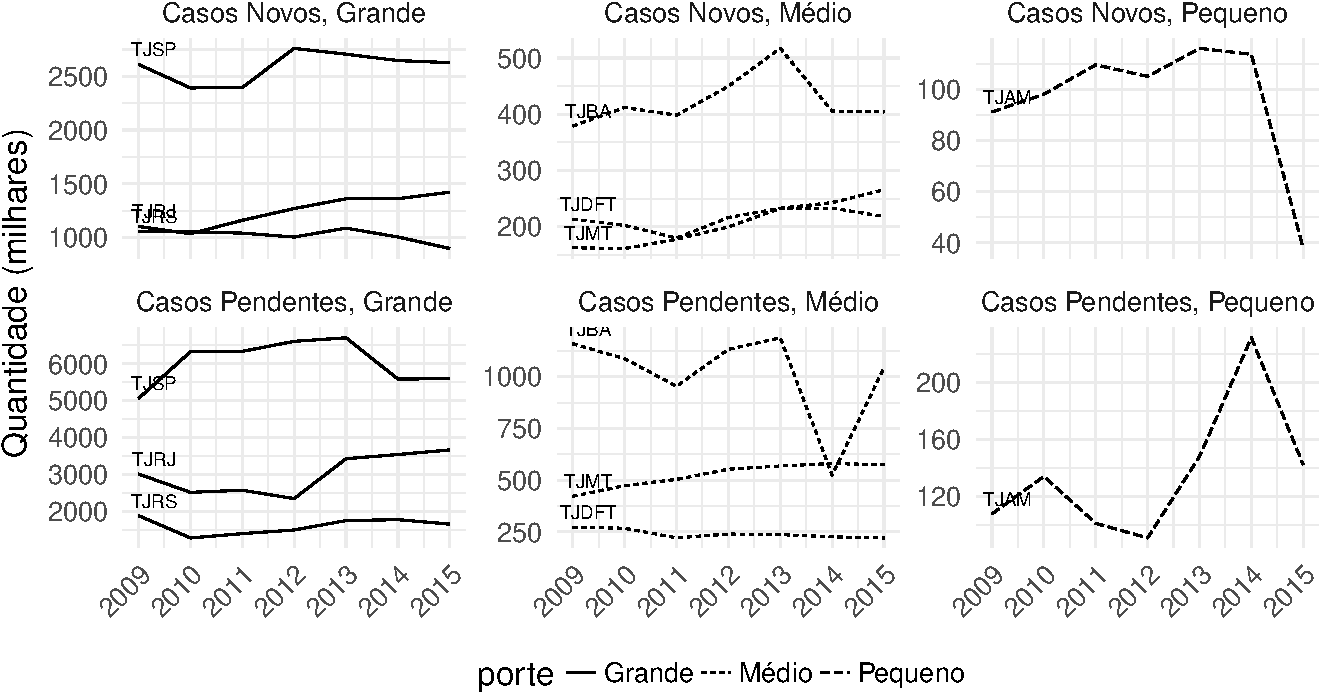
\includegraphics{bookdown_files/figure-latex/tempo-1.pdf}
\caption{\label{fig:tempo}Volume de casos novos e pendentes ao longo do
tempo nos tribunais de interesse. Fonte: Justiça em Números.}
\end{figure}

No RJN e no Módulo de Produtividade Mensal do CNJ, é possível observar
que assuntos envolvendo o direito do consumidor aparecem dentre os
assuntos mais frequentes, especialmente nas turmas recursais e juizados
especiais cíveis. No entanto, o próprio relatório enfatiza que a análise
não é completamente confiável. Nosso intuito é avançar nesse sentido,
produzindo novas estimativas.

Cada tribunal exigiu uma metodologia distinta para separação dos casos
consumeristas. A Subseção \ref{extracao} trata desse tema.

\subsection{Extração}\label{extracao}

As tarefas de extração e arrumação dos dados de processos digitais
passam por três fases: i) listagem dos processos, ii) download dos
arquivos de acompanhamento processual e autos do processo e iii)
transformação dos dados brutos em bases de dados analíticas. Em seguida,
descrevemos cada fase em detalhe.

Atualmente, existem três formas diferentes de listar processos judiciais
em estudos prospectivos. O primeiro envolve a composição de ofícios para
obtenção de dados diretamente dos tribunais. O segundo envolve a
obtenção de listas de processos nos Diários de Justiça Eletrônicos
(DJEs). O terceiro envolve a amostragem de números de processos. Nesse
estudo, utilizamos uma mistura de listas obtidas via ofício e por
extração dos DJEs.

A extração de dados dos tribunais escolhidos passou por duas atividades.
A primeira foi buscar cada número de processo da lista no sistema e-SAJ,
armazenando os resultados em arquivos HTML. A segunda foi ler e
classificar os arquivos de forma automática, transformando-os num
conjunto de bases passíveis de análise estatística. Os arquivos HTML,
após processados, apresentam informações de acompanhamento processual,
como:

\begin{itemize}
\tightlist
\item
  \textbf{Informações básicas}: classe/assunto (Res. 46 CNJ), vara,
  comarca, status, indicador de processo digital, local físico, entre
  outras.
\item
  \textbf{Partes}: contém nome do(s) réu(s), quando existe(m),
  advogado(s) e tipo de advogado (defesa pública ou particular).
\item
  \textbf{Movimentações}: datas, títulos e conteúdo de todas as
  movimentações do processo. São movimentações desde despachos simples,
  remessas e conclusos até atas de audiências, sentenças completas etc.
  Trata-se da base mais rica do tribunal, mas também a mais complexa de
  analisar.
\end{itemize}

O fluxo para leitura, limpeza e arrumação dos dados brutos foi descrito
na Figura \ref{fig:arrumacao}

\begin{figure}[htbp]
\centering
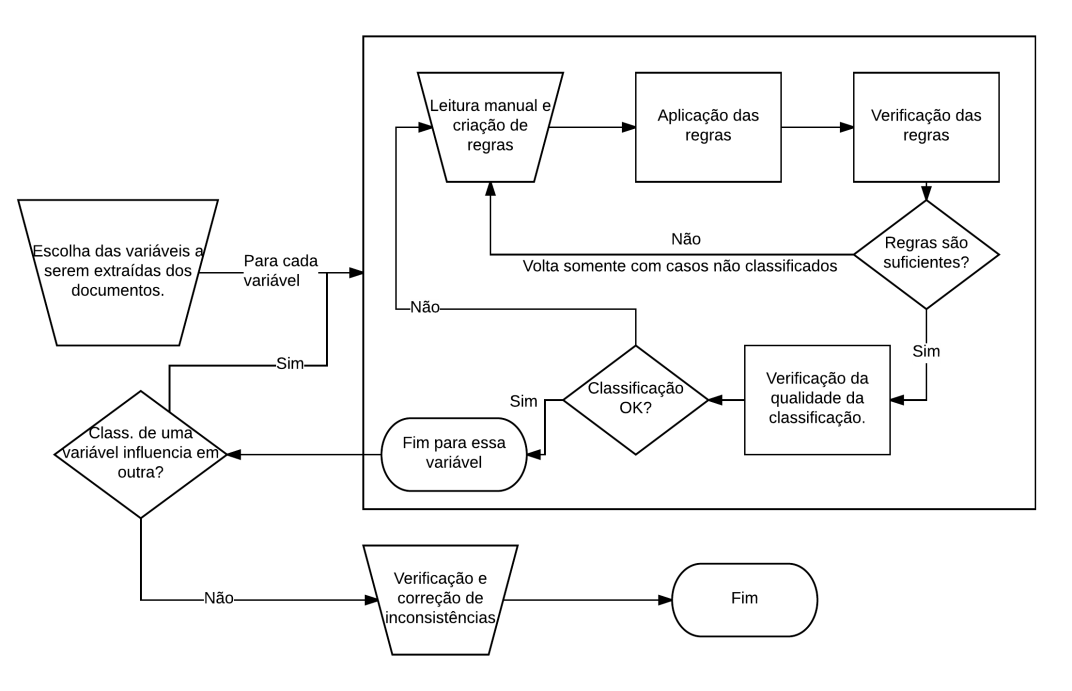
\includegraphics{imgs/classificacao.png}
\caption{Fluxo de leitura, limpeza e arrumação dos dados. Fonte:
Elaboração própria.}\label{fig:arrumacao}
\end{figure}

Em seguida, descrevemos as atividades realizadas para extração dos dados
em cada tribunal.

\subsubsection{Contatos com os tribunais}\label{contatos-tribunais}

O procedimento de realização de contatos com tribunais para extrair
processos judiciais é usualmente burocrático. A vantagem de burocratizar
extrações de dados é a prevenção de pedidos incoerentes, redução de
custos e o atendimento de demandas coerentes de forma correta e
completa. A desvantagem é que muitas vezes a extração pode demorar muito
e tornar algumas pesquisas inviáveis.

Especificamente sobre o presente projeto, as extrações eram complexas
pois envolviam altos volume de dados, já que estamos justamente atacando
o problema de litígios em massa na área consumerista. Por esse motivo,
nem sempre foi possível atender à demanda do projeto em tempo hábil.

Nos próximos parágrafos explicamos brevemente o histórico de contatos
com os tribunais e os resultados dos pedidos.

\textbf{TJAM}. Após os contatos com áreas de estatística, Tecnologia da
Informação e presidência do TJAM, ficamos inseguros com relação ao tempo
necessário para realizar a extração dos dados dentro do Tribunal. Por
isso, decidimos adotar uma estratégia de baixar os dados via \emph{web
scraping} (raspagem de dados) e amostragem.

\textbf{TJBA}. Os contatos com o TJBA não foram profícuos e por isso não
fomos capazes de obter extrações dos dados dos tribunais. No final,
também decidimos utilizar \emph{web scraping} e amostragem para acessar
os dados.

\textbf{TJDFT}. Realizamos algumas trocas de dados preliminares para
validar as extrações. Abrimos um canal de transferência de dados, mas
recebemos os dados somente no dia 22/06/2017. Por esse motivo, acabamos
não conseguindo analisar os dados para o presente relatório. No final,
utilizamos uma base enviada pelo DPJ baseada no Selo Justiça em Números.

\textbf{TJMS}. Após muitos contatos, a equipe de estatística solicitou
os telefones dos outros tribunais. Abrimos um canal de transferência de
dados, mas não recebemos os dados. No final, recebemos uma base do DPJ
baseada no Selo Justiça em Números. A base se refere ao TJMT. Por esse
motivo, fizemos a análise para o TJMT no lugar do TJMS.

\textbf{TJRJ}. O TJRJ sugeriu uma solução alternativa para extração dos
dados, a partir do envio dos dados do Justiça em Números. Após alguns
contatos com o DPJ e com o tribunal, a base foi recebida com sucesso.

\textbf{TJRS}. O TJRS foi o tribunal mais solícito para extração dos
dados. Além de responderem com rapidez e cordialidade, levantaram
dúvidas pertinentes sobre o pedido e nos auxiliaram com informações
adicionais.

\textbf{TJSP}. O contato com o TJSP também foi satisfatório. Por conta
do volume de dados foi necessário entrar em contato diversas vezes para
elaborar filtros adicionais e permitir a extração. O processo foi
facilitado por dois motivos: a ABJ já realizou projetos com a Secretaria
de Planejamento Estratégico (SEPLAN) no passado e está fisicamente
próxima do tribunal.

No final, fomos capazes de obter pelo menos uma base de dados por
tribunal. As bases de dados não são ideais pois não apresentam o mesmo
escopo, mas foram suficientes para levantamento dos maiores litigantes
em ações consumeristas.

A Tabela \ref{tab:tribunais} resume as características dos dados de cada
tribunal, após aplicação de todos os filtros. As bases prospectivas
obtidas via ofício têm escopo temporal de janeiro de 2009 até dezembro
2015, indexados pela data de distribuição. Os processos obtidos via web
scraping foram distribuídos a partir do ano de 2013. Os casos
retrospectivos do Selo Justiça em Números apresentam o escopo do Selo
para o ano de 2016.

\begin{longtable}{lllrlll}
\caption{Resumo dos dados dos tribunais utilizados para análise, após aplicação dos filtros de assuntos. Fonte: Justiça em Números.} \\
  \hline
Tribunal & Método Coleta & Tipo Levantamento & N & Cód. Assuntos & Filtro & Tipo Estudo \\
  \hline
TJAM & Web Scraping & Prospectivo & 14.777 & Não & Cível e criminal & Amostral \\
  TJBA & Web Scraping & Prospectivo & 7.222 & Não & Cível e criminal & Amostral \\
  TJDFT & Selo JN & Retrospectivo & 295.702 & Sim & Cível e criminal & Populacional \\
  TJMT & Selo JN & Retrospectivo & 513.757 & Sim & Cível e criminal & Populacional \\
  TJRJ & Selo JN & Retrospectivo & 1.759.509 & Sim & Cível e criminal & Populacional \\
  TJRS & Ofício & Prospectivo & 1.100.743 & Não & Cível & Populacional \\
  TJSP & Ofício & Prospectivo & 1.005.485 & Não & Consumerista & Populacional \\
   \hline
\hline
\label{tab:tribunais}
\end{longtable}

\subsection{Arrumação}\label{arrumacao}

A fase de arrumação dos dados considerou quatro etapas. As primeira e
segunda etapas têm como objetivo trabalhar com os assuntos corretamente
para classificar processos. As terceira e quarta etapas descrevem as
dificuldades e soluções para trabalhar com as partes nos processos.

\subsubsection{Assuntos - consumeristas}\label{assuntos}

Atualmente, existem duas formas de classificar um processo como
consumerista através de seu assunto. A primeira forma é chamada de
\textbf{clássica} e a segunda é chamada de \textbf{estatística}. Essas
definições foram criadas pela ABJ e podem ser vistas como um avanço
metodológico da pesquisa.

A forma clássica utiliza como base as Tabelas Processuais Unificadas
(TPUs) do CNJ, a partir de uma classificação manual dos assuntos que são
relacionados ao direito do consumidor. É possível resolver o problema
utilizando a TPU de assuntos, disponibilizada pelo CNJ, mas a principal
dúvida é se existem muitos processos de direito do consumidor que não
respeitam a classificação sugerida.

A forma estatística lista os assuntos processuais associados ao tema
``direito do consumidor'' usando como base os processos judiciais
disponíveis na ferramenta de pesquisa \emph{Consulta de Julgados de
Primeiro Grau} do TJSP.

Para isso, fizemos o levantamento de listas de sentenças do TJSP por
assunto e por ano, com base em todos assuntos descritos na TPUs. Em cada
uma dessas listas, detectamos a presença de um conjunto de
palavras-chave que estão associadas à justiça consumerista. Quando a
busca de termos retornou algum conteúdo, utilizamos o resultado para
classificar um assunto como ``potencialmente consumerista''.

O primeiro passo do estudo foi levantar a lista de assuntos na página do
TJSP. Em seguida, retiramos da lista aqueles assuntos da TPU que
provavelmente não estão associados à justiça consumerista. Esse filtro
foi feito retirando todos os assuntos que decorrem dos seguintes
assuntos gerais:

\begin{itemize}
\tightlist
\item
  DIREITO PENAL
\item
  DIREITO DA CRIANÇA DE DO ADOLESCENTE
\item
  DIREITO DO TRABALHO
\item
  DIREITO PROCESSUAL PENAL
\item
  DIREITO MARÍTIMO
\end{itemize}

O segundo passo do levantamento foi realizar uma pesquisa no site do
TJSP para cada ano e cada assunto obtido. Isso foi feito de forma por
\emph{web scraping} a partir da utilização das rotinas computacionais
desenvolvidas pela ABJ.

O terceiro passo da metodologia foi detectar as amostras em que aparece
um conjunto de palavras-chave relevantes nos processos consumeristas.
Para evitar o excesso de falsos positivos, utilizamos uma lista pequena
de termos muito importantes, como: CDC, Lei 8.078/90, Codigo de Defesa
do Consumidor e Lei 7.347/85 (Lei da ação civil pública).

Para avaliar a qualidade da classificação obtida de maneira puramente
jurimétrica, comparamos a tabela de assuntos obtida com uma lista de
assuntos classificada manualmente por pesquisadores da ABJ. A lista
obtida de forma automática foi chamada de \textbf{lista estatística},
enquanto a lista obtida manualmente foi chamada de \textbf{lista
clássica}.

A lista clássica possui 73 assuntos processuais, enquanto a lista
estatística possui 208. Apenas 4 assuntos aparecem na lista clássica,
mas não aparecem na estatística. Dentre eles, chama a atenção a presença
de um assunto do ramo ``DIREITO DO CONSUMIDOR''. O assuntos faltante,
``Clausulas Abusivas'', não foi contabilizado pois a busca por processos
desse assunto não retornou nenhum caso.

Para o relatório final, utilizamos somente o critério clássico para
filtrar os tipos processuais. A escolha foi feita para manter a
estabilidade nos resultados. A lista estatística foi utilizada para
obtenção dos dados do TJSP na fase de extração.

Sugerimos que o critério \emph{estatístico} seja investigado em detalhe
para i) reproduzir a pesquisa e comparar os resultados, e também para
realização de futuras pesquisas. Os códigos utilizados para definição
desse critério estão disponíveis publicamente.\footnote{Acessível pelo
  link: \url{https://github.com/abjur/whitelistTJSP}.}

\subsubsection{Assuntos - cifra oculta}\label{assuntos2}

Atualmente, a forma mais direta de identificar tipos de processos
judiciais é utilizando os chamados \emph{assuntos processuais}. Os
assuntos relacionam-se com as matérias discutidas em cada caso. Por
exemplo, um caso cível de indenização por dano moral poderia ter um
assunto ``Indenização por dano moral'', enquanto um processo falimentar
de uma empresa em Recuperação Judicial poderia ser classificado como
``Convolação de Recuperação Judicial em Falência''.

Nesse contexto, um importante passo foi dado com a Resolução 46 do CNJ
que criou as TPUs. As TPUs foram implantada em todas as Justiças, o que
permite a realização de análises que comparam diferentes tribunais.

As TPUs são estruturadas em formato de árvore. Isso significa que temos
assuntos genéricos e assuntos específicos, sendo que o assunto
específico é um ``filho'' do assunto genérico. As TPUs podem ter até
seis níveis hierárquicos de assuntos.

A Figura \ref{fig:tpu} mostra uma parte da árvore de assuntos relativa
ao Direito do Consumidor. Os números da imagem são códigos
identificadores dos assuntos. Note que, por exemplo, ``Inclusão Indevida
em Cadastro de Inadimplentes'' é um filho de ``Indenização por Dano
Moral'', que por sua vez é filho de ``Responsabilidade do Fornecedor''.

\begin{figure}[htbp]
\centering
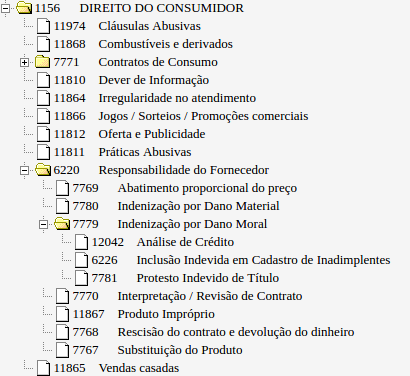
\includegraphics{imgs/tpu.png}
\caption{Árvore de assuntos relacionada ao Direito do Consumidor
(parcial). Último acesso em 27/06/2017.}\label{fig:tpu}
\end{figure}

O problema enfrentado atualmente é que, na prática, nem sempre os
processos são classificados com assuntos específicos. Assim, é possível
encontrar um caso que discute sobre ``Análise de Crédito'' classificado
como ``Responsabilidade do Fornecedor'', ou ainda ``Direito do
Consumidor''.

A existência de casos classificados com assuntos genéricos implica em
problemas para o levantamento do volume processual por assunto. Por
exemplo, considere que há interesse em conhecer o volume de processos
envolvendo ``Análise de Crédito''. Ao considerar somente os casos
classificados corretamente, estaríamos subestimando o real volume de
processos, pois os casos classificados em assuntos genéricos seriam
ignorados. Por outro lado, ao considerar todos os casos no levantamento,
incluindo os genéricos, estaríamos superestimando o real volume de
ações.

A possibilidade de subestimar sistematicamente o volume real de
processos de um certo tipo configura uma quantidade que chamamos de
\textbf{cifra oculta}. Dado um assunto específico, esse número pode ser
definido como a quantidade de processos com esse assunto, mas
classificados em assuntos genéricos.

A forma mais simples de estimar a cifra oculta é aplicando proporções.
No exemplo da análise de crédito, considere que temos uma base de dados
com todos os casos classificados com assuntos dentro da árvore do
Direito do Consumidor. Suponha também que todos os processos de análise
de crédito foram classificados ou corretamente, ou incorretamente como
``Direito do Consumidor''. Utilizando somente a parte da base que foi
classificada com assuntos específicos, calculamos a proporção de casos
\(p\) classificados como ``Análise de Crédito''. Assim, uma estimativa
do volume de processos de análise de crédito é dada por

\[
N = N_A + N_T \times p,
\]

onde

\begin{itemize}
\tightlist
\item
  \(N_A\) é o volume de casos classificados corretamente como ``Análise
  de Crédito''.
\item
  \(N_T\) é o volume total de casos classificados como ``Direito do
  Consumidor''. \(N_T \times p\) é a estimativa da cifra oculta.
\end{itemize}

Nesse cálculo, assumimos que o fato de um processo ser classificado de
forma genérica não tem relação alguma com o fato desse processo tratar
de análise de crédito. Esse é um conceito estatístico denominado
\textbf{independência} \citep{degroot2005optimal} e pode ou não ser
válido nos casos concretos.

O problema da cifra oculta é, essencialmente um caso de omissão de dados
\citep{rubin2004multiple}. Quando um estudo envolve omissão, a primeira
preocupação é com a existência de mecanismos para a geração dos dados e
se esse mecanismo estaria relacionado com os dados observados ou não
observados. Ignorar esse mecanismo pode gerar viés nos resultados.

É possível classificar os dados omissos em três tipos principais:

\begin{itemize}
\tightlist
\item
  \textbf{Missing completamente aleatório (MCAR)}. Não depende de
  nenhuma outra variável.
\item
  \textbf{Missing aleatório (MAR)}. A probabilidade de omissão depende
  somente das informações observadas.
\item
  \textbf{Missing não aleatório (MNAR)}. Outros casos.
\end{itemize}

Nas pesquisas da ABJ, até o momento, lidamos apenas com MCAR e MAR.
Nesses casos, podemos tratar os dados omissos como parâmetros a serem
estimados no modelo. Para trabalhar o caso MNAR é necessário utilizar
informações a priori sobre o problema específico ou plugar informações
de levantamentos anteriores (e.g.\textasciitilde{}uma amostra de
processos com assuntos classificados manualmente).

O caso MCAR é equivalente à aplicação da regra de proporcionalidade
definida acima. A única complicação é que o cálculo precisa ser
realizado para cada nível de generalização do assunto. Felizmente, é
possível estruturar as contas utilizando uma classe de modelos
estatísticos denominada \emph{rede Bayesiana} \citep{cozman2000credal}.

Uma rede Bayesiana é uma forma gráfica de representar a dependência de
variáveis aleatórias. No nosso caso, consideramos como variáveis
aleatórias cada um dos níveis da árvore da TPU, digamos,
\(N_1, N_2, \dots, N_6\), em que \(N_1\) é o nível mais genérico
(e.g.~Direito do Consumidor) e \(N_6\) é o nível mais específico
(e.g.~Análise de Crédito). Nos casos em que o nível mais específico não
ocorre no sexto nível, fazemos cópias do último nível disponível até
\(N_6\).

A rede da Figura \ref{fig:rb} representa a hierarquia dos níveis das
TPUs. Trata-se de uma rede bastante simples, que pode ser utilizada
diretamente para o cálculo dos volumes processuais.

\begin{figure}[htbp]
\centering
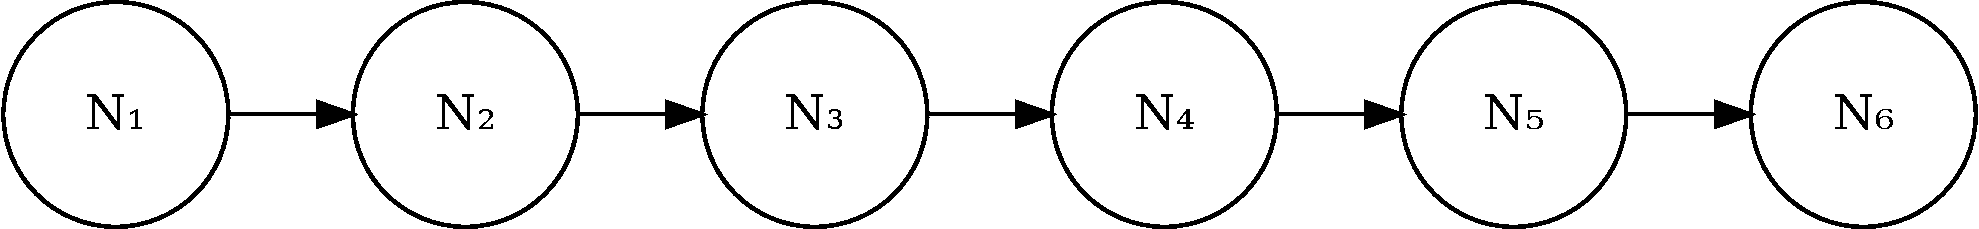
\includegraphics{imgs/08-metodologia_files/figure-latex/rb-1.pdf}
\caption{Rede Bayesiana representando a hierarquia dos níveis das TPUs.
Fonte: Elaboração própria.}\label{fig:rb}
\end{figure}

No caso MAR, podemos utilizar todos os dados disponíveis dos processos
para predizer o assunto real do processo. Para isso, qualquer técnica de
modelagem preditiva poderia ser utilizada.

Uma forma natural de realizar montar esses modelos é estendendo a rede
Bayesiana da Figura \ref{fig:rb}. Por exemplo, a rede da Figura
\ref{fig:rb2} considera que a classificação específica ou genérica de
determinado assunto processual depende da vara em que o processo é
distribuído. Outras variáveis poderiam ser consideradas para construir
um modelo mais completo.

\begin{figure}[htbp]
\centering
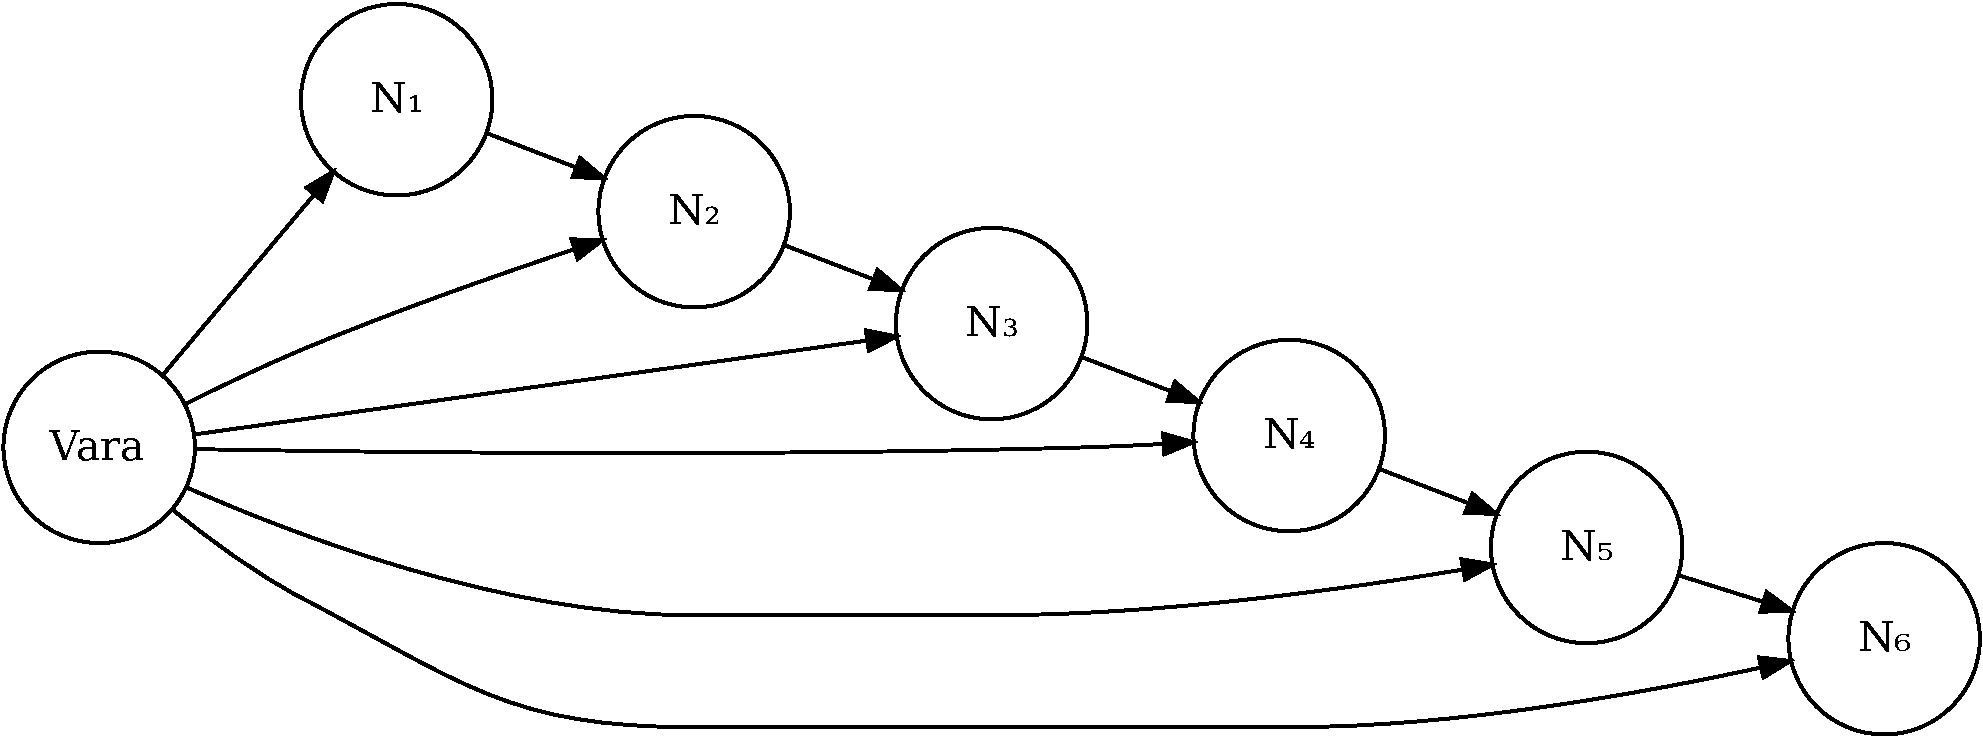
\includegraphics{imgs/08-metodologia_files/figure-latex/rb2-1.pdf}
\caption{Rede Bayesiana representando a hierarquia dos níveis das TPUs,
considerando também a vara.}\label{fig:rb2}
\end{figure}

O pacote escrito usando o software estatístico R chamado
\href{https://github.com/abjur/tpur}{tpur}, desenvolvido pela ABJ, pode
ser utilizado para executar duas tarefas:

\begin{itemize}
\tightlist
\item
  Baixar e estruturar as TPUs diretamente da fonte oficial do
  CNJ.\footnote{Acesso
    \href{https://www.cnj.jus.br/sgt/versoes.php}{neste link}. Último
    acesso em 26/06/2017.}
\item
  A partir de uma base de dados de processos, estimar o volume
  processual de um conjunto de assuntos com base em um modelo de redes
  Bayesianas.
\end{itemize}

Para o presente trabalho, tentamos aplicar a metodologia da cifra
oculta, mas acreditamos que a técnica ainda está instável para
apresentação no relatório final. Por isso incluímos a aplicação dessa
tecnologia como sugestão para aprimoramento do sistema.

\subsubsection{Empresas - filtro}\label{empresas1}

A classificação das empresas foi feita em duas partes. A primeira parte
refere-se à aplicação de filtros para separação de pessoas jurídicas e
físicas.

A aplicação dos filtros de pessoa física e jurídica é importante para
determinar qual a proporção de casos dos maiores litigantes em relação
ao total de casos envolvendo pessoas físicas no polo ativo e pessoas
jurídicas no polo passivo. Sem esse filtro, contaríamos vários casos de
execuções extrajudiciais de empresas contra pessoas, que não é nosso
interesse nesse caso específico.

Os filtros foram realizados a partir de aplicação de expressões
regulares aos nomes das partes. Por exemplo, um nome que termina com
``LTDA'' é certamente um caso de pessoa jurídica.

O problema da aplicação das expressões é que existem muitos casos
ambíguos: por exemplo, um nome terminando com ``SA'' não é
necessariamente uma sociedade anônima, pois pode ser um nome finalizando
com essas letras, como ``Heloísa''.

Por isso, foi necessário criar 32 expressões para organizar todas as
situações observadas nos dados. Além disso, criamos uma
\emph{whitelist}, que é uma lista de nomes sabidamente relacionados a
empresas, como Itaú, Bradesco etc.

O algoritmo utilizado para filtragem dos processos pelas partes foi
escrito com a linguagem de programação R e está descrito no Apêndice
\ref{codpfpj}.

\subsubsection{Empresas - limpeza e incorporações}\label{empresas2}

O segundo problema relativo ao levantamento de maiores litigantes é a
necessidade de lidar com vários nomes de empresas que se referem à mesma
empresa. As diferenças nos nomes podem aparecer por i) erros de escrita
ou ii) incorporações de empresas. Por exemplo, Telefonica hoje deve ser
considerada como Vivo ou Brasil Telecom, que é considerada Oi.

Ao todo, criamos mais de cem regras, considerando expressões regulares
utilizadas para identificar empresas e regras do tipo \emph{de-para}
para realizar as reclassificações relativas às incorporações. As regras
foram criadas a partir de pesquisas de notícias na internet para
encontrar atualizações sobre incorporações das empresas. Essas regras
foram importantes para identificar os maiores litigantes de forma
acurada.

No entanto, pode ser que algumas incorporações não tenham sido
consideradas. Isso pode ter ocorrido por dois motivos: i) insuficiência
de informações disponíveis na internet ou ii) possível arbitrariedade na
identificação das incorporações. O segundo problema é grave, pois,
dependendo do critério de classificação, como participação societária de
uma empresa em outra, ou grupo controlador, ou mesmo empresas de mesmo
segmento, a classificação pode mudar.

Um avanço metodológico da presente pesquisa está no fato desses códigos
de classificação serem replicáveis. Isso significa que o mesmo código
pode ser utilizado para reclassificar empresas em pesquisas futuras. O
algoritmo utilizado para classificação dos nomes das empresas foi
escrito com a linguagem de programação R e está descrito no Apêndice
\ref{codpj}. Convidamos o leitor a criticar os critérios utilizados e
propor sugestões de mudanças.

\subsection{Métricas de avaliação}\label{metricas-de-avaliacao}

Como descrito nas Seções anteriores, um dos resultados da pesquisa é a
elaboração de propostas de solução que impactam nos principais
indicadores de gestão do judiciário. Monitorar o efeito de políticas
públicas em indicadores de litigiosidade é essencial para avaliar se a
política atingiu seus objetivos.

Uma das principais métricas nesse sentido é a taxa de congestionamento.
Historicamente, a mesma já considerou duas metodologias distintas de
cálculo. A mais recente é obtida através da fórmula

\[
T_C = \frac{N_P}{N_B + N_P} \times 100\%,
\]

onde \(N_P\) é o número de casos pendentes e \(N_B\) é o número de casos
baixados no final do período. Note que essa taxa não leva em conta a
quantidade de casos novos diretamente. Se o número de casos pendentes ao
final do período é igual a zero, a taxa de congestionamento é igual
zero. Se o número de casos baixados no período é zero, a taxa de
congestionamento vale 100\%.

Um avanço metodológico recente do CNJ é métrica chamada \textbf{índice
de atendimento à demanda} (IAD), que é dado por

\[
T_{IAD} = \frac{N_B}{N_N}\times 100\%,
\]

onde \(N_N\) é o número de casos novos e \(N_B\) é o número de casos
baixados. Essa taxa tem duas propriedades interessantes: i) quanto maior
a quantidade de baixados, maior é a taxa e ii) quanto menor a quantidade
de processos que entram, maior é a taxa. Por desconsiderar os casos
pendentes, IAD é um índice que reflete a produtividade de um tribunal
naquele ano.

O único problema do IAD é que essa quantidade não tem um valor máximo
conhecido. Assim, seria complicado definir metas relativas ao IAD, pois
não temos um valor de corte para atingir.

Uma possibilidade de evoluir o IAD é criando um \emph{IAD normalizado}.
Primeiro, pode-se esperar que

\[
N_P^{t} \approx N_P^{t-1} + N_N^{t} - N_B^{t},
\]

onde \(t\) é o ano base considerado para o cálculo do volume processual.
O valor é aproximado pois as estatísticas passadas pelos tribunais não
são completamente confiáveis e existem muitas variáveis (e.g.~migrações
de sistema, mudança nos critérios de levantamento, processos suspensos
etc) que influcenciam nas medições.

De fato, observando as variáveis do RJN, é possível estudar a
distribuição da razão entre \(N_P^t\) e \(N_P^{t-1} + N_N^{t}-N_B^{t}\).
A Figura \ref{fig:comparacao} mostra, a título de exemplo, a comparação
entre o número de casos pendentes observados e o número de casos
pendentes calculado com base no número de casos pendentes do ano
anterior e dos casos novos e baixados no ano corrente. O levantamento
considera como base os dados relativos aos casos de conhecimento em
primeiro grau na Justiça Estadual. Observa-se que na maior parte dos
casos (162 casos no total, por considerar 27 UFs por 6 anos) a
quantidade calculada subestima a quantidade observada. Em 26 casos as
duas quantidades são exatamente iguais, e a razão entre as quantidades
fica concentrada no ponto 1. Ainda nesse exemplo, se fizermos a razão
entre o total de casos pendentes observados e o total de casos pendentes
calculados, encontramos o valor de 103,5\%.

\begin{figure}[htbp]
\centering
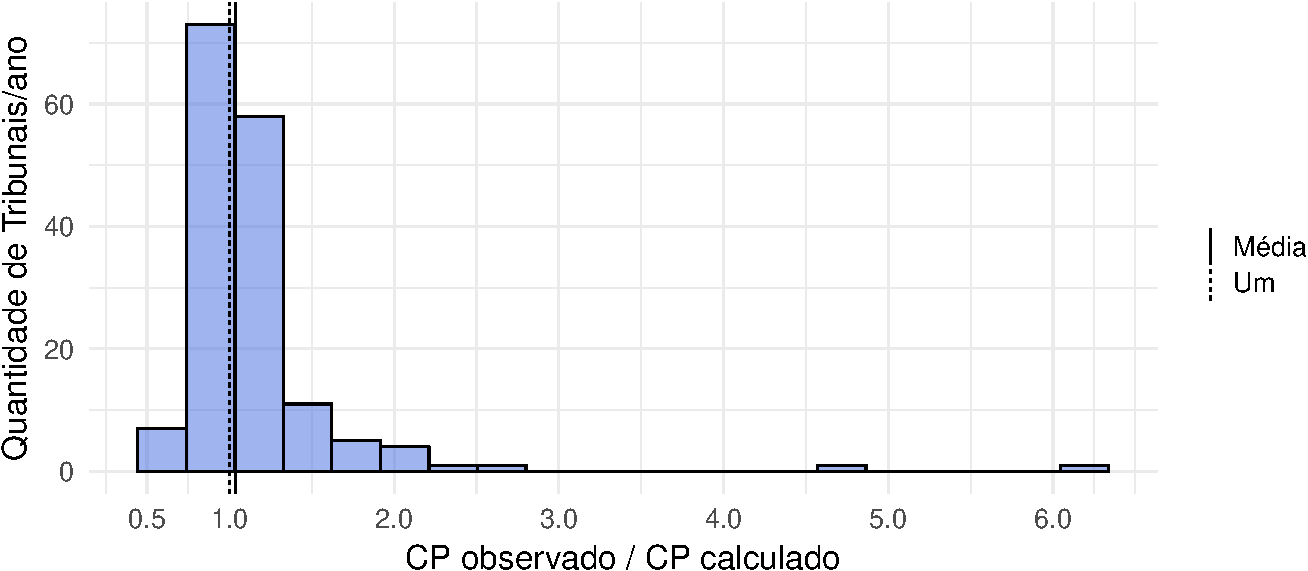
\includegraphics{bookdown_files/figure-latex/comparacao-1.pdf}
\caption{\label{fig:comparacao}Comparação da quantidade de casos pendentes
observada e calculada pela fórmula aproximada, considerando apenas casos
de conhecimento de primeiro grau. Fonte: Justiça em Números.}
\end{figure}

Fazendo \(N_P^t = 0\) obtemos o valor máximo aproximado de processos
baixados \(N_B^{t*}\). Assim, o valor máximo de casos baixados é dado
pela quantidade de casos pendentes no ano anterior, somada ao volume de
casos novos no ano corrente, o que faria o número de casos pendentes no
ano corrente chegar a zero.

\[
\max_{N_B^t}T_{IAD}^t = \frac{N_N^{t} + N_P^{t-1}}{N_N^t} \geq 1
\]

Por esse motivo o IAD original pode assumir valores maiores que 100\%.
Uma possibilidade é dividir o IAD pelo máximo aproximado, obtendo

\[
T_{IADN}^t = \frac{T^t_{IAD}}{\max_{N_B^t}T_{IAD}^t} = \frac{N_B^t}{N_N^t + N_P^{t-1}}.
\]

Chamamos essa taxa de \textbf{IADN - Índice de Atendimento da Demanda
Normalizado}. Essa taxa pode ser interpretada como a quantidade de
baixados sobre o total que poderia ser baixado. Assim como na taxa de
congestionamento, seria possível adaptar essa quantidade para uma
quantidade líquida, retirando do denominador a contagem de processos
suspensos ou arquivados provisoriamente.

O IADN tem as mesmas vantagens do IAD (diretamente proporcional aos
baixados, inversamente proporcional aos entrados), mas varia
aproximadamente entre zero e um. No entanto, o IADN também considera os
casos pendentes e, portanto, falha em medir a produtividade instantânea
dos tribunais.

É interessante notar que o IADN corresponde exatamente ao complemento da
taxa de congestionamento utilizada antes de 2015 pelo CNJ.\footnote{É
  possível verificar a definição em \url{https://goo.gl/LBaJQZ}. Último
  acesso em 15/08/2017.} A fórmula atual foi adaptada, pois o CNJ passou
a coletar o quantitativo de casos pendentes no final do período, ao
invés do inicio. Essa alteração tem a vantagem de considerar os
processos reativados no estoque.

A Tabela \ref{tab:iadn} e a Figura \ref{fig:iadn2} mostram o IADN
calculado para o ano de 2015 e o IADN ao longo dos anos,
respectivamente, considerando somente processos de primeiro grau não
criminais e não fiscais, nos Tribunais escolhidos na pesquisa. Nos
tribunais de médio e grande porte, com exceção do TJDFT, o IADN é
estável e encontra-se entre de 35\% e 40\%. Já no TJDFT essa métrica
encontra-se muito acima dos demais, com 68\%, possivelmente por conta da
baixa quantidade de casos pendentes no Tribunal, relativa à quantidade
de casos novos. No TJAM, a taxa varia muito e já alcançou o valor máximo
dentre todos os Tribunais analisados, mas atualmente tem o valor mínimo
do IADN. Isso indica que a taxa no TJAM não é confiável.

\begin{longtable}{lllrrrrr}
\caption{IADN de 2015 para processos de primeiro grau não criminais nos Tribunais considerados na pesquisa. Fonte: Justiça em Números.} \\
  \hline
Tribunal & Região & Porte & Ian & Iadn & Novos & Baixados & Pendentes 2014 \\
  \hline
TJAM & Norte & Pequeno & 73,5\% & 10,3\% & 37.761 & 27.767 & 231.237 \\
  TJMT & Centro-Oeste & Médio & 112,9\% & 35,4\% & 265.614 & 299.863 & 580.474 \\
  TJRS & Sul & Grande & 108,9\% & 36,4\% & 897.469 & 976.941 & 1.784.106 \\
  TJSP & Sudeste & Grande & 115,0\% & 36,8\% & 2.627.933 & 3.021.298 & 5.586.281 \\
  TJRJ & Sudeste & Grande & 130,1\% & 37,2\% & 1.421.339 & 1.848.862 & 3.545.465 \\
  TJBA & Nordeste & Médio & 93,0\% & 40,5\% & 404.084 & 375.919 & 524.629 \\
  TJDFT & Centro-Oeste & Médio & 138,5\% & 68,1\% & 218.231 & 302.322 & 225.703 \\
   \hline
\hline
\label{iadn}
\end{longtable}

\begin{figure}[htbp]
\centering
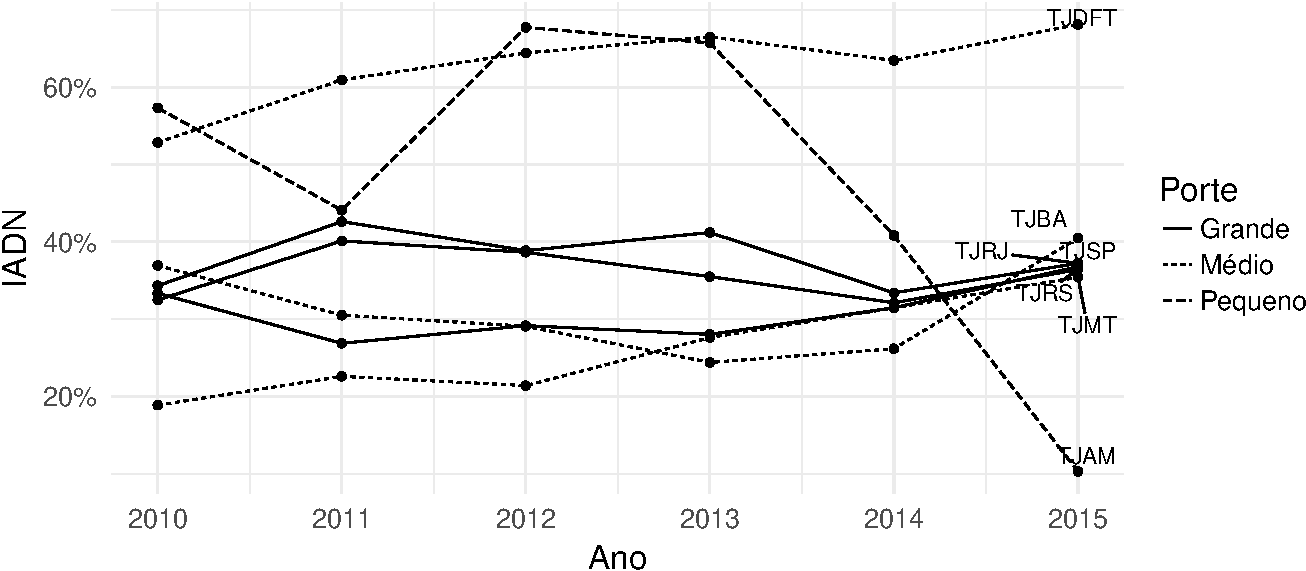
\includegraphics{bookdown_files/figure-latex/iadn2-1.pdf}
\caption{\label{fig:iadn2}IADN ao longo dos anos para os tipos processuais e
tribunais de interesse. Fonte: Justiça em Números.}
\end{figure}

Uma forma de generalizar o IAD e o IADN (taxa de congestionamento
antiga) é considerar um fator de multiplicação \(\lambda \in [0,1]\), e
chamaremos a taxa resultante de \textbf{IAD relativo} (IADR):

\[
T_{IAD}^t(\lambda) = \frac{N_B^t}{N_N^t + \lambda N_P^{t-1}}.
\]

Dessa forma, se \(\lambda = 1\), temos o IADN e, se \(\lambda = 0\),
temos o IAD. O valor de \(\lambda\) pode ser escolhido de acordo com um
tribunal de referência, por exemplo, ou obtido através de um
procedimento de teoria da decisão, adicionando maior ou menor peso aos
casos pendentes do período anterior de acordo com a preferência do CNJ
em priorizar a produtividade instantânea (IAD) ou a produtividade
completa (IADN) dos tribunais.

A Figura \ref{fig:iadn3} mostra o IADR calculado para os tribunais
escolhidos na pesquisa, considerando diferentes valores de \(\lambda\).
É interessante notar que a posição relativa de alguns tribunais, como o
TJBA muda ao considerar diferentes valores de \(\lambda\).

\begin{figure}[htbp]
\centering
\includegraphics{bookdown_files/figure-latex/fig:iadn3-1.pdf}
\caption{(\#fig:fig:iadn3)IADR calculado para os tribunais da pesquisa
considerando diferentes valores de \(\lambda\). Fonte: Justiça em
Números.}
\end{figure}

O IADR ainda não foi trabalhado com dados reais e pode precisar de
estudos aprofundados para a escolha do valor de \(\lambda\). No entanto,
uma vez que este generaliza os conceitos do IAD e da taxa de
congestionamento, pode ser sempre considerado em estudos de
produtividade dos tribunais.

Assim, temos a informação de qual a população de casos que podem ser
alvo de soluções estratégicas. São 25 milhões de casos pendentes, sendo
que aproximadamente metade desses casos estão nos tribunais considerados
na análise. Temos também o indicador IADR para avaliar o impacto de
possíveis ações.

\section{Parte propositiva}\label{parte-propositiva}

Como mencionado na introdução, com o intuito de sistematizar nosso
estudo e deixá-lo mais próximo da elaboração de políticas públicas,
obtivemos nossas hipóteses de interesse respondendo a perguntas
organizadas sob dois questionamentos principais:

\begin{enumerate}
\def\labelenumi{\arabic{enumi}.}
\tightlist
\item
  O que pode ser feito para agilizar a tramitação dos processos
  consumeristas e reduzir o estoque de processos?
\item
  O que pode diminuir o número de processos consumeristas que entram no
  judiciário?
\end{enumerate}

Os seis eixos de investigação foram elaborados procurando dividir as
conclusões de pesquisa em subtópicos diretamente relacionados à
elaboração de alguma política pública.

As entrevistas tiveram o objetivo de alinhar as hipóteses da pesquisa e
dividir experiências. Uma entrevista geralmente tem como retorno a visão
de um tipo de profissional ou de uma entidade sobre determinado tema,
que pode ou não ser concordante com outras pessoas.

Com o intuito de obter opiniões plurais e variadas, a ABJ elencou para
entrevistas diferentes profissionais, como juízes e advogados, bem como
diferentes entidades, como empresas do setor de varejo e bancário e a
Secretaria Nacional do Consumidor (SENACON).

As entrevistas foram conduzidas de maneira informal e não foram gravadas
nem registradas de forma sistemática. Os resultados das conversas foram
anotados pela equipe da ABJ para confrontamento com as hipóteses
levantadas.

No Apêndice \ref{questionario}, apresentamos o questionário base para
realização das entrevistas. Observe que algumas questões são específicas
para alguns tipos de profissionais ou entidades.

Realizamos ao todo cinco reuniões:

\begin{itemize}
\tightlist
\item
  Equipe de advogados especializados no novo CPC.
\item
  Presidente da Secretaria Nacional do Consumidor (SENACON).
\item
  Juízas assessoras da Corregedoria do TJSP.
\item
  Diretoria jurídica do Grupo Pão de Açúcar.
\item
  Diretoria jurídica do Itaú-Unibanco.
\end{itemize}

As anotações das reuniões foram adicionadas no Apêndice \ref{reunioes}.

Após as reuniões, decidimos que os eixos de investigação mais
importantes são aqueles que tratam dos litígios potenciais e não do
estoque atual. A importância dada a temas como IRDR, impactos do novo
CPC e otimização das filas de trabalho nos tribunais foi baixa, enquanto
incentivos para litigar ou para cometimento de ilícitos abriram amplo
espaço para debate.

Notamos que pode existir um distanciamento de opiniões entre as empresas
e o tribunal. Para as empresas entrevistadas, o consumidor é parte do
problema de um fenômeno de hiperlitigiosidade, entrando com ações em
excesso por conta de incentivos de advogados oportunistas, de leis ou da
atuação do judiciário. Para os juízes entrevistados, o volume de ações é
baixo frente ao volume de conflitos gerados pelas empresas.

Apesar dessa discordância, foi possível identificar alguns consensos.
Nas conversas, todos afirmaram que aumentar o incentivo à conciliação
dentro do processo não surtiria efeitos positivos. Também mencionaram
que a melhor solução para o problema seria aprimorar os meios de
composição extrajudicial e alinhar incentivos para que os processos não
cheguem ao judiciário.

Os eixos de investigação foram montados para dividir as conclusões de
pesquisa em subtópicos diretamente relacionados à elaboração de alguma
política pública.

Ao final da primeira fase do projeto, os eixos de investigação foram
ordenados de acordo com uma lista de prioridade, com auxílio do
Departamento de Pesquisas Judiciárias - DPJ-CNJ. Na segunda fase,
fizemos um corte de escopo para focar no levantamento dos maiores
litigantes. O único eixo de investigação completamente desenvolvido na
pesquisa foram os canais de composição extrajudicial. Em seguida,
apresentamos uma descrição mais aprofundada sobre esse tema.

\subsection{Canais de composição
extrajudicial}\label{canais-de-composicao-extrajudicial}

Uma alternativa à litigância no caso da justiça consumerista é a
resolução de conflitos diretamente entre as partes, especialmente por
muitas empresas já contarem com canais de comunicação direta com seus
clientes. É importante considerar políticas públicas que utilizem essa
alternativa pois ela possui um baixo custo de implementação para o
judiciário.

Os canais de comunicação extrajudicial são importantes ferramentas de
composição pré-processual. Dentre eles, destacamos os canais fornecidos
pelas próprias empresas fornecedoras de serviços e/ou produtos (SACs) e
os canais disponibilizados por terceiros, como a Fundação Procon e o
site Consumidor.gov.

O Decreto n.º 6.523/2008 determina que as ligações para os SACs são
gratuitas e não importam em qualquer ônus para o consumidor. O serviço
deve funcionar 24 horas por dia, 7 dias por semana e deve disponibilizar
opções de contato com o atendente, reclamação e cancelamento de
contratos e serviços.

As informações solicitadas pelo consumidor devem ser prestadas
imediatamente e as reclamações devem ser resolvidas no prazo máximo de 5
dias, a contar do registro. A resposta do fornecedor de serviços deve
ser clara e objetiva, além de abarcar todos os pontos da solicitação do
consumidor.

Quando o contato feito pelo consumidor versar sobre serviço não
solicitado ou cobrança indevida, a cobrança deve ser suspensa
imediatamente, salvo se o fornecedor indicar o instrumento por meio do
qual o serviço foi contratado ou comprovar que o valor é efetivamente
devido.

A Fundação Procon (Fundação de Proteção e Defesa do Consumidor) também é
uma importante ferramenta de comunicação posta ao alcance do consumidor.
Os consumidores que se sentirem lesados podem elaborar reclamações
fundamentadas para a Fundação Procon, que detém legitimidade para
aplicar multa às empresas infratoras.

Os canais extrajudiciais também se apresentem formalmente como boas
ferramentas para solução dos conflitos. No entanto, existem obstáculos
óbvios no caminho para a negociação extrajudicial: o conflito de
interesse intrínseco aos problemas do consumidor pode provocar uma
indisposição a negociação oriunda de ambas as partes. Para atenuar este
problema, é possível utilizar canais públicos de comunicação entre
empresas e consumidores, já que a transparência do canal fornece às
partes incentivos à negociação bem sucedida.

Nesse sentido, existem algumas iniciativas já implementadas. A SENACON
disponibilizou o portal consumidor.gov.br para negociação entre clientes
e empresas cadastradas. Além disso, existem portais privados tais como o
``Reclame Aqui''. Nestes serviços, estatísticas de desempenho nas
negociações de todas as empresas são disponibilizados ao público,
incentivando as empresas a performarem bem com relação a esses
indicadores.

Uma limitação deste tipo de estratégia encontra-se na voluntariedade na
realização de negociações. Mesmo que as taxas de resolução do
consumidor.gov.br estejam majoritariamente acima de 60\%, os
consumidores podem simplesmente não procurar esses meios pelos mais
diversos fatores, tais como a desinformação e o descrédito.

Como outra alternativa, a superação dos obstáculos da negociação
extrajudicial pode ser realizada pelos próprios tribunais. O Centros
Judiciários de Solução de Conflitos e Cidadania (CEJUSC) instituídos
pela Res. 125 do CNJ oferecem aos interessados a oportunidade de
negociar um acordo, que se aceito será homologado pelo juiz, antes do
ajuizamento da disputa.

Considerando essas opções, os objetivos deste eixo de investigação
concentram-se em caracterizar as tentativas de solução antes da
judicialização da queixa. Em particular, listamos alguns
questionamentos:

\begin{enumerate}
\def\labelenumi{\arabic{enumi}.}
\tightlist
\item
  Os canais de comunicação disponibilizados pelas empresas são pouco
  utilizados com relação ao volume de litígios?
\item
  A procura por mecanismos de conciliação extrajudiciais por parte dos
  requerentes é pequena com relação ao volume de litígios?
\item
  Nos casos de negociação extrajudicial observados, a maior parte dos
  litígios são evitados?
\end{enumerate}

Esse tema foi também o mais discutido nas reuniões com especialistas.
Identificamos um consenso de que a melhor forma de reduzir o estoque dos
tribunais é fazer com que menos litígios apareçam no futuro, e a melhor
forma de fazer isso é através da composição extrajudicial.

Nos resultados, apresentamos uma análise utilizando a base de dados do
canal de conciliação consumidor.gov.br. Esses resultados foram
utilizados como insumo para uma das propostas principais no capítulo de
sugestões.

\hypertarget{resultados}{\chapter{Resultados}\label{resultados}}

As análises do capítulo de resultados seguiram um roteiro de perguntas,
considerando o objetivo principal da pesquisa. Em cada tribunal
analisado, conduzimos as investigações respondendo às questões abaixo,
na ordem em que o encadeamento das respostas foi mais natural.

\begin{enumerate}
\def\labelenumi{\arabic{enumi}.}
\tightlist
\item
  Quem são os maiores litigantes?
\item
  Os 30 maiores litigantes concentram qual percentual do total de
  processos?
\item
  Sobre características dos maiores litigantes:

  \begin{itemize}
  \tightlist
  \item
    Quais são os 5 setores com maior quantidade de processos?
  \item
    Quais são os 10 assuntos processuais mais comuns em cada setor?
  \item
    Os volumes processuais apresentam algum tipo de padrão temporal?
  \end{itemize}
\end{enumerate}

O roteiro limitou-se às cifras mencionadas acima (5 setores, 10 assuntos
processuais e 30 litigantes) apenas para tornar a exposição mais clara.
Conforme verificado a seguir, esses números foram capazes de descrever o
comportamento de grande quantidade dos processos. Mesmo assim, para os
casos não comentados nesse capítulo, o apêndice contém versões menos
resumidas das tabelas.

Em alguns tribunais, os mecanismos de seleção impossibilitam análises
temporais. Isso acontece porque os dados utilizados na premiação do Selo
Justiça em Números não representam adequadamente os processos
distribuídos em um ano. Os dados obtidos na ocasião desse prêmio
representam adequadamente os processos que receberam carga e aqueles
processos que estavam em aberto no momento da coleta. Por conta disso,
fizemos análises temporais e conduzimos estudos prospectivos nos estados
de São Paulo, Rio Grande do Sul, Amazonas e Bahia.

\section{TJRS}\label{tjrs}

Conforme mencionado na seção de metodologia, o Tribunal de Justiça do
Rio Grande do Sul forneceu os dados de todos os processos cíveis
distribuídos entre 2009 e 2016. Nesta subseção, descrevemos os
resultados obtidos nesse estado.

\subsection{Os maiores litigantes do Rio Grande do
Sul}\label{os-maiores-litigantes-do-rio-grande-do-sul}

Similar ao identificado nos demais estados, a empresa com maior número
de processos no Rio Grande do Sul foi o grupo de empresas de telefonia
Oi Telecomunicações, com 13,0\% dos litígios. Entretanto, destoando dos
demais casos consumeristas analisados nesse relatório, o segundo maior
litigante é a administradora de cadastro de inadimplentes Serasa, com
8,8\% dos processos.

\begin{longtable}{lrll}
\caption{30 maiores litigantes da Justiça Estadual do Rio Grande do Sul. Fonte: Tribunal de Justiça de Rio Grande do Sul.} \\
  \hline
Nome da Empresa ou Grupo & Frequência & Percentual & Percentual Acumulado \\
  \hline
Oi
Telecomunicações & 142900 & 13,0\% & 13,0\% \\
  Serasa Experian & 96803 & 8,8\% & 21,8\% \\
  Itaú & 46323 & 4,2\% & 26,0\% \\
  Boa Vista Spc & 45816 & 4,2\% & 30,1\% \\
  Bradesco & 40106 & 3,6\% & 33,8\% \\
  Claro & 39942 & 3,6\% & 37,4\% \\
  Banco
Votorantim & 37488 & 3,4\% & 40,8\% \\
  Cdl Porto
Alegre & 36097 & 3,3\% & 44,1\% \\
  Vivo & 32037 & 2,9\% & 47,0\% \\
  Santander & 26491 & 2,4\% & 49,4\% \\
  Banco Do Brasil & 26369 & 2,4\% & 51,8\% \\
  Banrisul & 21874 & 2,0\% & 53,8\% \\
  Companhia
De Estadual
De Energia
Elétrica & 16719 & 1,5\% & 55,3\% \\
  Rio Grande
Energia & 14309 & 1,3\% & 56,6\% \\
  Aes Sul & 13935 & 1,3\% & 57,9\% \\
  Banco Pan & 13073 & 1,2\% & 59,1\% \\
  Tim & 13024 & 1,2\% & 60,3\% \\
  Unimed & 12588 & 1,1\% & 61,4\% \\
  Banco Finasa & 9625 & 0,9\% & 62,3\% \\
  Aymore & 9514 & 0,9\% & 63,1\% \\
  Corsan & 8370 & 0,8\% & 63,9\% \\
  Lider & 7939 & 0,7\% & 64,6\% \\
  Hsbc & 7570 & 0,7\% & 65,3\% \\
  Sky & 7178 & 0,7\% & 66,0\% \\
  Bmg & 7051 & 0,6\% & 66,6\% \\
  Magazine Luiza & 6345 & 0,6\% & 67,2\% \\
  Net & 6316 & 0,6\% & 67,8\% \\
  Tam & 5911 & 0,5\% & 68,3\% \\
  Gol & 4829 & 0,4\% & 68,7\% \\
  Ford & 4809 & 0,4\% & 69,2\% \\
   \hline
\hline
\label{unnamed-chunk-5}
\end{longtable}

A lista dos maiores litigantes é composta apenas por bancos, empresas de
telefonia e administradores de cadastro de inadimplentes até a posição
de número 12. Nessas categorias, os maiores litigantes são os bancos
Itaú, Banco do Brasil, Bradesco, Santander, Votorantim e Banrisul, as
empresas de telefonia são a Tim, Vivo, Claro e Oi e as administradoras
de cadastro são a Boa Vista e a Serasa.

A partir da décima segunda posição, destacam-se novos setores da
economia. Na décima terceira posição vê-se a seguradora Líder,
administradora do seguro DPVAT, com 4,2\% dos processos, e a partir
dessa marca começam a aparecer empresas de energia, luz e água, como a
Rio Grande Energia, AES Sul, CEEE e Corsan. Além dessas empresas, novos
bancos, como o Banco PAN (antes chamado Banco PanAmericano), BOSCH, BMG
e FINASA\footnote{Incorporado ao Banco Bradesco Financiamentos em 2002}.

Os 30 maiores litigantes acumulam 69,2\%, mas pudemos compreender melhor
a origem dos demais litígios ao agruparmos os processos por setor da
economia das demandadas. Analisando dessa forma, concluímos que 67,0\%
dos processos concentram-se no setores financeiro, telecomunicações e
administradoras de cadastro de inadimplentes. Os três primeiros setores
possuem proporções acima de 10\% dos processos e caracterizam um ponto
de corte na distribuição de processos por empresa: a partir delas, a
fatia consumida por cada instituição orbita em 1\%. Nas esferas
restantes, cujas demandadas concentram menos de 10\% do total,
destacam-se as concessionárias de serviços básicos, como energia, gás,
água e esgoto, e empresas de seguros, com 4,5\% e 3,9\% dos processos,
respectivamente.

\begin{longtable}{lrll}
\caption{5 maiores passivos consumeristas na Justiça Estadual do Rio Grande do Sul. Fonte: Tribunal de Justiça de Rio Grande do Sul.} \\
  \hline
Area & Frequência & Percentual & Percentual Acumulado \\
  \hline
Instituições
Financeiras & 308171 & 28,0\% & 28,0\% \\
  Telecomunicações & 246293 & 22,4\% & 50,4\% \\
  Administradoras
De Cadastro De
Inadimplentes & 183300 & 16,7\% & 67,0\% \\
  Concessionárias
De Serviços
Básicos & 53793 & 4,9\% & 71,9\% \\
  Companhias De
Seguro & 37952 & 3,4\% & 75,4\% \\
   \hline
\hline
\label{unnamed-chunk-7}
\end{longtable}

Considerando o interesse em qualificar certas instituições como
demandadas em massa pelos litigantes, partimos para uma análise que
buscou averiguar a existência de padrões temporais que expliquem o
volume de casos de um certo grande litigante levantado nas tabelas
anteriores. Analisando o volume mensal de distribuições de cada tipo de
processo, foi possível identificar padrões.

\begin{figure}[htbp]
\centering
\includegraphics{bookdown_files/figure-latex/f1-1.pdf}
\caption{\label{fig:f1}Volume processual consumerista no Rio Grande do Sul
ao longo do tempo e separado por setor econômico. Fonte: Tribunal de
Justiça de Rio Grande do Sul.}
\end{figure}

O padrão mais claro revelou-se nos processos relacionados à empresas
administradoras de banco de dados. No ano de 2013 essas empresas
experienciaram uma litigância em massa nunca antes identificada.
Enquanto a média de processos por ano, desconsiderando 2013, foi de
10641 processos, em 2013 foram distribuídos 119455 processos. Nessa
época, algumas instituições associaram esse aumento repentino à
litigância incentivada pelos escritórios de advocacia, contudo é um fato
que a quantidade de processos diminuiu com o tempo, indicando que a
massa de questões foi causada por alguma característica particular da
época.

\begin{figure}[htbp]
\centering
\includegraphics{bookdown_files/figure-latex/f3-1.pdf}
\caption{\label{fig:f3}Volume processual ao longo do tempo no Rio Grande do
Sul contra empresas administradoras de cadastro de inadimplentes. Fonte:
Tribunal de Justiça de Rio Grande do Sul.}
\end{figure}

Outros padrões temporais se destacaram, mas, diferentemente do observado
nas administradoras de cadastro de inadimplentes, nenhuma série sugere
que as questões tratadas nos processos contra a instituição em questão
já foram superadas. No caso dos fabricantes de produtos eletrônicos e
transporte aéreo, por exemplo, o que ocorre é exatamente o contrário: os
processos contra essas empresas estão em ascensão. Em relação às
empresas aéreas, o aumento deve-se principalmente à Gol, cujo número de
litígios vêm numa tendência de subida desde 2012, mas também é
influenciada pelo aumento de processos da TAM de 2010 para 2012.

\begin{figure}[htbp]
\centering
\includegraphics{bookdown_files/figure-latex/f4-1.pdf}
\caption{\label{fig:f4}Volume processual ao longo do tempo no Rio Grande do
Sul contra fabricantes de produtos eletrônicos e companhias aéreas.
Fonte: Tribunal de Justiça de Rio Grande do Sul.}
\end{figure}

Um outro padrão detectado nos gráficos de volume processual contra o
tempo diz respeito aos setores com uma quantidade aproximadamente
constante de processos por mês.f Isso acontece com os processos contra
administradoras de planos de Saúde, concessionárias de Energia, Gás e
Esgoto, empresas de telecomunicações e empresas de Seguros. Essas quatro
esferas, embora tenham experienciado crescimentos desde 2010, apresentam
séries estáveis de processos por mês, pelo menos a partir de algum
ponto. Dentre os aumentos identificados, destacou-se o patamar atingido
pelas empresas de telecomunicações: são registrados aproximadamente
5.500 novos casos por mês.

\begin{figure}[htbp]
\centering
\includegraphics{bookdown_files/figure-latex/f5-1.pdf}
\caption{\label{fig:f5}Volume processual ao longo do tempo no Rio Grande do
Sul das áreas em que identificou-se um aumento (telecomunicações,
concessionárias de serviços básicos, planos de saúde e seguros). Fonte:
Tribunal de Justiça de Rio Grande do Sul.}
\end{figure}

O último grupo de padrões temporais identificados diz respeito aos
processos que experienciaram um aumento o qual já foi revertido durante
o período de estudo. Pertencem à esse grupo as instituições financeiras,
empresas relacionadas à recuperação de crédito e supermercados.

\begin{figure}[htbp]
\centering
\includegraphics{bookdown_files/figure-latex/f6-1.pdf}
\caption{\label{fig:f6}Volume processual ao longo do tempo no Rio Grande do
Sul nas áreas em que identificou-se estabilidade (instituições
financeiras, supermercados e companhias de recuperação de crédito).
Fonte: Tribunal de Justiça de Rio Grande do Sul.}
\end{figure}

\subsection{Causas de pedir}\label{causas-de-pedir}

Nesta seção estudamos as causas de pedir mais frequentes aos maiores
litigantes separando-os de acordo com a área em que atuam.

\subsubsection{Bancos e Instituições
Financeiras}\label{bancos-e-instituicoes-financeiras}

\begin{longtable}{lrll}
\caption{10 maiores causas de pedir contra instituições financeiras do Rio Grande do Sul. Fonte: Tribunal de Justiça de Rio Grande do Sul.} \\
  \hline
Causa de pedir (Assunto) & Frequência & Percentual & Percentual Acumulado \\
  \hline
Interpretação / Revisão de Contrato & 112163 & 36,4\% & 36,4\% \\
  Bancários & 46333 & 15,0\% & 51,4\% \\
  Indenização por Dano Moral & 32196 & 10,4\% & 61,9\% \\
  Reparação de Danos & 30175 & 9,8\% & 71,7\% \\
  Contratos de Consumo & 13512 & 4,4\% & 76,1\% \\
  Expurgos Inflacionários / Planos Econômicos & 13251 & 4,3\% & 80,4\% \\
  Financiamento de Produto & 12649 & 4,1\% & 84,5\% \\
  Seguro & 10505 & 3,4\% & 87,9\% \\
  Inclusão Indevida em Cadastro de Inadimplentes & 7532 & 2,4\% & 90,3\% \\
  Indenização por Dano Material & 7178 & 2,3\% & 92,6\% \\
   \hline
\hline
\label{unnamed-chunk-9}
\end{longtable}

Com relação às causas de pedir, a maior parte das ações contra
instituições financeiras tratam de ``Interpretação/ Revisão de
Contrato'', com 36,4\% dos processos. No presente contexto, uma análise
textual de alguns casos mostrou que a maior parte dos casos desse tipo
trata dos contratos de prestação de serviços a clientes, como manutenção
de contas correntes e poupanças.

A segunda causa mais frequente dos processos contra instituições
bancárias é a classificação geral ``Bancários'', com 15,0\%. Segundo a
Tabela Processual Unificada, esse vértice deriva três outros assuntos
possíveis: ``Empréstimo Consignado'',``Expurgos Inflacionários ou Planos
Econômicos'' e ``Tarifas'', mas o erro de classificação pode ou não
considerar essa estrutura.

A terceira causa mais frequente dos processos contra instituições
bancárias é a classificação geral ``Indenização por Dano Moral'', com
10,4\% dos pleitos. Essa é uma classificação geral e, segundo a TPU,
admite duas ramificações: ``Inclusão Indevida em Cadastro de
Inadimplentes'' e ``Protesto Indevido de Título''. Novamente é razoável
observar que o erro de classificação pode ou não considerar a hierarquia
da Tabela para ocorrer, mas é possível imaginar que processos por danos
morais à uma instituição bancária na justiça civil estejam relacionados
a cadastros indevidos em bases de inadimplentes.

A quarta causa mais frequente de ações contra instituições bancárias é
``Reparação de Danos'', com 9,8\% dos processos. Essa é uma
classificação que não consta nas TPU's do primeiro grau da Justiça
Estadual. Conforme constatado durante essa pesquisa, a classificação
está presente apenas no Tribunal do Rio Grande do Sul, mas nesse caso é
bastante frequente. Por esse motivo, concluiu-se que ``Reparação de
Danos'' é uma classificação alternativa para processos cíveis de danos
morais ou materiais.

A quinta causa mais frequente dos processos contra instituições
financeiras são litígios por ``Expurgos Inflacionários/ Planos
Econômicos'', com 4,4\% dos processos. Essa é uma classificação
específica, derivada da classificação ``Bancários''. Processos desse
tipo pedem indenizações pela atuação de instituições bancárias na
ocasião dos planos econômicos brasileiros: Bresser, Verão, Real e os
dois planos Collor.

A sexta causa mais frequente dos processos contra instituições
financeiras se dão por ``Contratos de Consumo'', com 4,3\% dos
processos. Essa é uma classificação geral do segundo nível de altura da
TPU do primeiro grau da Justiça Estadual. Sob esse nível, estão vários
tópicos irrelevantes para instituições financeiras, como ``Serviços
Hospitalares'',``Turismo'' e ``Transporte Aéreo'', porém alguns tópicos
sugerem sobre o que se tratam os processos classificados dessa forma.
Além da classificação ``Bancários'', já mencionada acima, abaixo de
``Contatos de Consumo'' aninham-se as classificações ``Cartões de
Crédito'',``Consórcio'',``Plano de Saúde'',``Seguro'' e ``Financiamento
de Produto'', que são plausíveis no contexto financeiro, pois as
principais instituições bancárias do Brasil costumeiramente oferecem
estes serviços aos seus clientes.

A sétima causa mais frequente dos processos contra instituições
financeiras são aqueles por ``Financiamento de Produto'', com 4,1\% dos
casos. Essa é uma classificação específica, aninhada sobre a
classificação anterior, ``Contratos de Consumo''. Esses processos estão
relacionados aos contratos de financiamento de produtos diversos.

A oitava causa mais frequente dos processos contra instituições
financeiras são processos com o assunto ``Seguros'', com 3,4\% dos
casos. Essa classificação é similar à classificação ``Financiamento de
Produto'', mas versa sobre contratos de seguro.

A nona causa mais frequente dos processos contra instituições
financeiras são processos com o assunto ``Inclusão Indevida em Cadastro
de Inadimplentes'', com 2,4\% dos casos. Esse assunto é uma
especialização da classificação geral ``Indenização por Dano Moral'',
previamente detectada como a terceira maior causa de litigar contra
instituições bancárias.

A décima causa mais frequente dos processos contra instituições
financeiras são processos com o assunto ``Indenização por Dano
Material'', com 2,3\% dos casos. Segundo a TPU, esse assunto é uma
especialização da classificação geral ``Responsabilidade do
Fornecedor'', que carece de uma aplicabilidade mais direta no caso
financeiro.

Juntas, as dez maiores causas de pedir contra instituições financeiras
abarcam mais de 90\% dos litígios. Entretanto, para efetivamente
consolidá-las como causas de pedir recorrentes no judiciário brasileiro,
buscamos por padrões temporais da sua ocorrência, bem como padrões
relacionados as instituições demandadas.

Analisando os gráficos do volume processual contra o tempo, concluiu-se
que alguns assuntos processuais estão em tendência de queda, enquanto
outros estabilizam-se. Processos relacionados à planos econômicos, por
exemplo, devido à sua natureza factual, tendem a desaparecer com o tempo
e é isso que se observou. Fora o caso extremo mencionado, também notamos
o declínio de processos sobre financiamento de produtos e contratos de
consumo, que decaem em direção ao zero. Por outro lado, existe classe de
processos que estabilizam-se em torno de uma média, como os processos
relacionados à interpretação e revisão de contratos, à classificação
geral ``Bancários'', às indenizações morais e materiais e aos processos
de ``Reparação de Danos''.

\begin{figure}[htbp]
\centering
\includegraphics{bookdown_files/figure-latex/f7-1.pdf}
\caption{\label{fig:f7}Volumes processuais ao longo do tempo dos processos
contra instituições financeiras no Rio Grande do Sul. Fonte: Tribunal de
Justiça de Rio Grande do Sul.}
\end{figure}

Com relação às instituições demandadas, observamos uma diferença
significativa entre a distribuição dos assuntos do banco BV e a
distribuição dos assuntos nas outras instituições bancárias. Nessa
instituição, a maior parte dos processos corresponde ao assunto
``Interpretação/ Revisão de Contrato''. De fato, existem instituições
com padrões similares, como o Banco Itaú, FINASA e o Banco PAN, mas
nenhuma é tão díspar quanto o Banco Votorantim.

\begin{figure}[htbp]
\centering
\includegraphics{bookdown_files/figure-latex/f8-1.pdf}
\caption{\label{fig:f8}Distribuições das causas de pedir dos processos
contra instituições financeiras do Rio Grande do Sul, separadas por
empresa. Fonte: Tribunal de Justiça de Rio Grande do Sul.}
\end{figure}

A despeito dessa diferença nas proporções de assuntos entre os bancos,
todos eles experienciaram o mesmo aumento de processos de interpretação
ou revisão de contrato no anos de 2012 e 2013. De toda forma, a
intensidade variou de maneira similar ao que acontece na distribuição de
assuntos.

\begin{figure}[htbp]
\centering
\includegraphics{bookdown_files/figure-latex/f9-1.pdf}
\caption{\label{fig:f9}Número de processos contra instituições financeiras
que versam sobre interpretação ou revisão de contratos, separado por
data de distribuição e institução. Fonte: Tribunal de Justiça de Rio
Grande do Sul.}
\end{figure}

\subsection{Empresas de
telecomunicações}\label{empresas-de-telecomunicacoes}

De todos os processos contra empresas de telecomunicações, 34,0\% têm
como assunto ``Telefonia'', e esse é o assunto mais frequente. Segundo a
TPU, essa é uma classificação geral que pode possuir três ramificações:
processos relacionados à assinatura básica mensal, cobrança indevida de
ligações e pulsos excedentes.

O segundo assunto processual mais frequente nos processos consumeristas
é o já mencionado ``Reparação de Danos'', com 18,1\% dos casos. Esse
assunto está relacionado à processos de danos morais e materiais, que
figuram nas posições 3 e 8, colocando o tópico ``danos
morais/materiais'' com 38.1\% do total de casos referentes à empresas de
telefonia.

Após os processos derivados de danos causados aos consumidores, o
próximo tópico mais frequente nos tribunais é a cobrança indevida de
tarifas, com 10,0\% dos casos. Não sem relação com esse assunto, o
próximo tópico mais procurado pelos consumidores relaciona-se à
interpretação e revisão de contrato, com 3,5\% dos casos, também
relacionado com a sétima posição, rescisão do contrato.

Considerando os assuntos mencionados nessa seção, conduzimos uma análise
das diferenças nas distribuições de assuntos de cada demandada. Assim
como no caso dos bancos, verificamos uma diferença relevante nas
distribuições de assuntos: processos sobre interpretações ou revisões de
contrato aparecem apenas no grupo empresarial Tim e empresas
relacionadas ao grupo Oi são mais demandadas em processos do assunto
geral ``Telefonia''. Embora esse último assunto seja uma classificação
não específica, possivelmente ela está relacionada a processos
decorrentes de falhas no serviço, pois ``Cobrança Indevida de Serviços''
também é um assunto que se destaca em empresas do grupo Oi. No geral, as
demais empresas apresentam proporções similares de processos de
Telefonia, Indenização por Dano Moral e Reparação de Danos, que são as
outras formas de classificar danos morais e materiais na justiça
estadual gaúcha.

\begin{figure}[htbp]
\centering
\includegraphics{bookdown_files/figure-latex/f10-1.pdf}
\caption{\label{fig:f10}Distribuições das causas de pedir dos processos
contra empresas de telefonia no Rio Grande do Sul, separadas por
empresa. Fonte: Tribunal de Justiça de Rio Grande do Sul.}
\end{figure}

Assim como existem diferenças no volume de cada assunto processual,
também identificamos padrões temporais distintos em cada uma das maiores
litigantes de telefonia. O volume processual associado ao grupo Oi é
muito maior do que os demais, com exceção de processos relacionados à
Inclusão Indevida em Cadastro de Inadimplentes e Interpretação ou
Revisão de Contratos, e, em geral, o volume processual da Oi está em
ascensão, exceto pelos casos relacionados à Telefonia e Reparação de
Danos. Nesse último caso vale a pena notar que o número total de casos
está diminuindo, possivelmente por tratar-se de uma classificação antiga
que está caindo em desuso, dando lugar às classificações ``Indenização
por Dano Moral'' e ``Inclusão Indevida em Cadastro de Inadimplentes''.

Ainda sobre os padrões temporais, destacou-se também a diferença dos
processos relacionados à TIM. Das empresas de telefonia com maior número
de litígios na Justiça Estadual do Rio Grande do Sul ela é a única cujo
volume processual relacionado à Inclusão Indevida em Cadastro de
Inadimplentes não está subindo, mas pudemos notar uma concentração de
processos relacionados à Interpretação e Revisão de Contratos.

\begin{figure}[htbp]
\centering
\includegraphics{bookdown_files/figure-latex/f11-1.pdf}
\caption{\label{fig:f11}Número de processos contra empresas de
telecomunicações ao longo do tempo separado por empresa. Fonte: Tribunal
de Justiça de Rio Grande do Sul.}
\end{figure}

\subsection{Admnistradores de cadastro de
inadimplentes}\label{admnistradores-de-cadastro-de-inadimplentes}

A menos de empresas não contabilizadas neste estudo, todos os processos
contra administradores de crédito concentraram-se em apenas quatro
instituições: Serasa Experian, com 52,8\% dos casos, Boa Vista SCPC, com
77,8\% dos casos, CDL de Porto Alegre, com 97,5\%, e o Serviço de
Proteção ao Crédito (SPC), com 100,0\%.

Do mesmo modo, apenas quatro assuntos processuais acumularam mais de
90\% dos casos, sendo todos eles relacionados direta ou indiretamente
com o cadastro indevido nas bases de inadimplentes. 36,0\% são processos
por ``Indenização de Danos Morais'' e os próximos três assuntos,
``Cadastro de Análise de Crédito'', ``Inclusão Indevida em Cadastro de
Inadimplentes'' e ``Registro em Cadastro de Análise de Crédito'' versam
sobre a mesma matéria e juntos concentraram 55\% dos processos.

Ao contrário do identificado nos assuntos adiante, os padrões temporais
existentes nas empresas administradoras de banco de dados limitam-se ao
já identificado: os processos concentram-se em 2013, para todas as
demandadas. Um desvio a esse padrão apareceu nos processos classificados
como ``Inclusão Indevida em Cadastro de Inadimplentes'', que
experienciaram um aumento gradual no número de processos até 2013,
quando esse número atingiu seu máximo.

\begin{figure}[htbp]
\centering
\includegraphics{bookdown_files/figure-latex/f12-1.pdf}
\caption{\label{fig:f12}Número de processos contra empresas administradoras
de cadastro de inadimplentes ao longo do tempo e separado por tipo de
processo. Fonte: Tribunal de Justiça de Rio Grande do Sul.}
\end{figure}

\subsection{Companhias de Luz, Água e
Esgoto}\label{companhias-de-luz-agua-e-esgoto}

Da mesma forma que observamos nos processos contra administradoras de
cadastros de inadimplentes, os processos contra empresas concessionárias
de serviços básicos como energia, gás e água concentraram-se em quatro
companhias.

\begin{longtable}{lrll}
\caption{4 Maiores Litigantes concessionárias de serviços básicos no estado do Rio Grande do Sul. Fonte: Tribunal de Justiça de Rio Grande do Sul.} \\
  \hline
Nome da Empresa ou Grupo & Frequência & Percentual & Percentual Acumulado \\
  \hline
Companhia
De Estadual
De Energia
Elétrica & 16719 & 31,1\% & 31,1\% \\
  Rio Grande
Energia & 14309 & 26,6\% & 57,7\% \\
  Aes Sul & 13935 & 25,9\% & 83,6\% \\
  Corsan & 8370 & 15,6\% & 99,1\% \\
   \hline
\hline
\label{unnamed-chunk-14}
\end{longtable}

A distribuição de assuntos é similar às identificadas anteriormente, mas
a separação por empresa faz mais sentido. Certos processos, como
``Fornecimento de Energia Elétrica'', só apareceram vinculadas à certas
empresas. Nesse aspecto, pudemos dividir as empresas deste segmento
econômico em dois grupos: as empresas de energia e a CORSAN, empresa Rio
Grandense de Saneamento. Indenizações por Dano Moral são frequentes em
todas empresas, mas Fornecimento de Energia Elétrica não apareceu
vinculada à CORSAN, evidentemente, assim como processos discutindo a
Metodologia de Reajuste das Tarifas e Indenizações por Danos Materiais.

\begin{figure}[htbp]
\centering
\includegraphics{bookdown_files/figure-latex/f13-1.pdf}
\caption{\label{fig:f13}Distribuições das causas de pedir contra
concessionárias de serviços básicos separadas por empresa.}
\end{figure}

Com relação aos padrões temporais, a conclusão geral foi que a maior
parte dos processos deveu-se a ilícitos cometidos pontualmente, já que
distribuem-se ao longo dos anos com muitos picos e períodos com baixo
volume processual. Já os processos que lidam com a questão do serviço
propriamente dito são mais estáveis: os processos relacionados ao
Fornecimento de Água contra a CORSAN estão crescendo, mas a média mensal
de processos distribuídos orbita os 50 processos/mês, e os processos
relacionados ao Fornecimento de Energia Elétrica não tiveram variação no
tempo.

\begin{figure}[htbp]
\centering
\includegraphics{bookdown_files/figure-latex/f14-1.pdf}
\caption{\label{fig:f14}Número de processos contra concessionárias de
serviços básicos ao longo do tempo separado por tipo de processo. Fonte:
Tribunal de Justiça de Rio Grande do Sul.}
\end{figure}

\section{TJRJ}\label{tjrj}

Conforme mencionado na seção de metodologia, os processos enviados pelo
Tribunal de Justiça do Rio de Janeiro foram utilizados originalmente
para a premiação do Selo Justiça em Números. Por conta disso, as
análises desse tribunal foram separadas de acordo com os mecanismos de
seleção dos processos enviados ao CNJ.

A qualidade da administração dos dados do TJRJ foi mensurada utilizando
três tipos de processos, que estão discriminados na base enviada pelo
CNJ:

\begin{enumerate}
\def\labelenumi{\arabic{enumi}.}
\tightlist
\item
  Processos baixados entre 01/01/2015 e 31/07/2016.
\item
  Processos em tramitação no dia 31/07/2016.
\item
  Processos com alguma movimentação ou utilização no mês de agosto de
  2016.
\end{enumerate}

\subsection{Os maiores litigantes do Rio de
Janeiro}\label{os-maiores-litigantes-do-rio-de-janeiro}

Similar ao identificado em outros estados, o maior litigante no estado
do Rio de Janeiro pertence ao setor das telecomunicações. O grupo de
empresas ligadas à Oi Telefonia concentra 12,8\% de todos os processos
consumeristas do estado. Nas primeiras posições, destacam-se também as
instituições bancárias, sendo mais expressivos os grupos empresariais
ligados ao Banco Itaú e ao Banco Bradesco, com 7,0\% e 4,8\% dos
processos, respectivamente.

\begin{longtable}{lrll}
\caption{30 maiores litigantes da justiça consumerista no estado do Rio de Janeiro. Fonte: Selo Justiça em Números.} \\
  \hline
Nome da Empresa ou Grupo & Frequência & Percentual & Percentual Acumulado \\
  \hline
Oi
Telecomunicações & 226062 & 12,8\% & 13\% \\
  Itaú & 122621 & 7,0\% & 20\% \\
  Claro & 107584 & 6,1\% & 26\% \\
  Bradesco & 84886 & 4,8\% & 31\% \\
  Light & 79794 & 4,5\% & 35\% \\
  Vvar & 76598 & 4,4\% & 40\% \\
  Santander & 70181 & 4,0\% & 44\% \\
  Nextel & 60209 & 3,4\% & 47\% \\
  Vivo & 54017 & 3,1\% & 50\% \\
  Tim & 49274 & 2,8\% & 53\% \\
  Ampla & 46035 & 2,6\% & 56\% \\
  Sky & 37303 & 2,1\% & 58\% \\
  Banco do Brasil & 30068 & 1,7\% & 59\% \\
  Cedae & 27090 & 1,5\% & 61\% \\
  Bmg & 22592 & 1,3\% & 62\% \\
  Net & 22473 & 1,3\% & 63\% \\
  Ricardoeletro & 22309 & 1,3\% & 65\% \\
  Leader & 21489 & 1,2\% & 66\% \\
  Unimed & 19284 & 1,1\% & 67\% \\
  Cnova & 15028 & 0,9\% & 68\% \\
  Banco Pan & 13843 & 0,8\% & 69\% \\
  Banco
Votorantim & 12024 & 0,7\% & 69\% \\
  Amil & 11537 & 0,7\% & 70\% \\
  Ibi & 10489 & 0,6\% & 71\% \\
  B2w & 9348 & 0,5\% & 71\% \\
  Tam & 9044 & 0,5\% & 72\% \\
  Hsbc & 8392 & 0,5\% & 72\% \\
  Gol & 8385 & 0,5\% & 73\% \\
  Consul & 8059 & 0,5\% & 73\% \\
  Qualicorp & 8029 & 0,5\% & 74\% \\
   \hline
\hline
\label{unnamed-chunk-19}
\end{longtable}

A principal particularidade do estado do Rio encontra-se na quinta
posição: a Light, distribuidora de energia, concentra 4,5\% dos
processos consumeristas do estado, abaixo apenas das maiores
instituições bancárias e empresas de telefonia. Além disso, também
destaca-se o fato do grupo Via Varejo, uma empresa varejista, aparecer
na lista das 10 maiores litigantes consumeristas, episódio não
identificado em nenhum outro estado.

Os 30 maiores litigantes acumulam aproximadamente 74\%, mas pudemos
compreender melhor a origem dos demais litígios ao agruparmos os
processos por setor da economia das demandadas. Analisando dessa forma,
concluímos que que 75,0\% dos processos concentram-se no setores
financeiro, fornecimento de energia e água, telecomunicações, seguros e
varejo. As quatro primeiras classes possuem proporções acima de 5\% dos
processos e caracterizam um ponto de corte na distribuição de processos
por empresa: abaixo dos 5\%, a fatia consumida por cada instituição
orbita os 1\%. Nessa nova classe de processos, cujas demandadas
concentram menos de 5\% do total, destacam-se as empresas de varejo e
seguros, com 6,4\% e 2,8\% do total de processos, respectivamente.

\begin{longtable}{lrll}
\caption{5 setores econômicos com maior quantidade de processos consumeristas no estado do Rio de Janeiro. Fonte: Selo Justiça em Números.} \\
  \hline
Area & Frequência & Percentual & Percentual Acumulado \\
  \hline
Telecomunicações & 574943 & 32,7\% & 32,7\% \\
  Instituições
Financeiras & 428275 & 24,3\% & 57,0\% \\
  Concessionárias
de serviços
básicos & 154413 & 8,8\% & 65,8\% \\
  Varejo & 113099 & 6,4\% & 72,2\% \\
  Companhias de
seguro & 48869 & 2,8\% & 75,0\% \\
   \hline
\hline
\label{unnamed-chunk-20}
\end{longtable}

\subsection{Causas de pedir}\label{causas-de-pedir-1}

Nesta seção estudamos as causas de pedir mais frequentes dentre os
maiores litigantes separando-os de acordo com a área em que atuam.

\subsubsection{Bancos e Instituições
Financeiras}\label{bancos-e-instituicoes-financeiras-1}

No TJRJ, 3 assuntos da TPU contemplam 94,2\% do total de processos
consumeristas contra bancos e instituições financeiras.

\begin{longtable}{lrll}
\caption{8 causas de pedir consumeristas mais frequentes conta instituições financeiras no estado do Rio de Janeiro. Fonte: Selo Justiça em Números.} \\
  \hline
Descrição & Frequência & Percentual & Percentual Acumulado \\
  \hline
Indenização por Dano Moral & 263145 & 65,5\% & 65,5\% \\
  Responsabilidade do Fornecedor & 95041 & 23,6\% & 89,1\% \\
  Bancários & 20508 & 5,1\% & 94,2\% \\
  Indenização por Dano Material & 18640 & 4,6\% & 98,8\% \\
  Contratos de Consumo & 4553 & 1,1\% & 100,0\% \\
  Telefonia &  91 & 0,0\% & 100,0\% \\
  Expurgos Inflacionários / Planos Econômicos &  35 & 0,0\% & 100,0\% \\
  Transporte Aéreo &   8 & 0,0\% & 100,0\% \\
   \hline
\hline
\label{unnamed-chunk-22}
\end{longtable}

O assunto mais frequente, com 65,5\% dos processos, diz respeito à
indenizações por danos morais. Em seguida, tem-se a classificação
genérica ``Responsabilidade do Fornecedor'', com 23,6\% dos processos.
Essa é uma classificação genérica que pode ser particularizada para
``Indenização por Dano Moral''.

A partir do terceiro assunto mais frequente questões relativas à
prestação de serviços bancários passaram a aparecer. A classificação
genérica ``Bancários'', que aparece em 5,1\% dos processos, segundo a
TPU é uma classificação relacionada a empréstimos consignados, expurgos
inflacionários e tarifas. Logo em seguida, o quarto assunto mais
frequente se manteve no mesmo sentido: ``Contratos de Consumo'' é uma
classificação acima de ``Bancários'' e que abarca outros serviços
prestados por instituições financeiras, como financiamentos, cartões de
crédito e consórcios.

\subsubsection{Telecomunicações}\label{telecomunicacoes}

Similar ao identificado nos processos contra instituições bancárias, as
causas de pedir contra empresas de telefonia também são bastante
polarizadas: 97,5\% dos processos estão concentrados em três assuntos.
Esses assuntos, inclusive, são similares aos assuntos mais frequentes do
setor bancário.

Dentre os processos consumeristas, 94,1\% versam, direta ou
indiretamente, sobre indenizações por danos morais, sendo esta
exatamente a classificação mais frequente e ``Responsabilidade do
Fornecedor'', uma de suas versões mais genéricas, a segunda mais
frequente.

\begin{longtable}{lrll}
\caption{9 assuntos consumeristas mais frequentes contra empresas de telecomunicações no estado do Rio de Janeiro. Fonte: Selo Justiça em Números.} \\
  \hline
Descrição & Frequência & Percentual & Percentual Acumulado \\
  \hline
Indenização por Dano Moral & 424183 & 74,9\% & 74,9\% \\
  Responsabilidade do Fornecedor & 108793 & 19,2\% & 94,1\% \\
  Indenização por Dano Material & 19502 & 3,4\% & 97,5\% \\
  Telefonia & 12003 & 2,1\% & 99,7\% \\
  Contratos de Consumo & 1360 & 0,2\% & 99,9\% \\
  Bancários & 550 & 0,1\% & 100,0\% \\
  Transporte Aéreo &   5 & 0,0\% & 100,0\% \\
  Crimes contra as Relações de Consumo &   1 & 0,0\% & 100,0\% \\
  Transporte Terrestre &   1 & 0,0\% & 100,0\% \\
   \hline
\hline
\label{unnamed-chunk-24}
\end{longtable}

\subsubsection{Empresas de energia, gás, água e
esgoto}\label{empresas-de-energia-gas-agua-e-esgoto}

Seguindo o padrão dos setores analisados até então, as empresas
distribuidoras de água, gás e energia também possuem uma grande
polarização dos assuntos. Os três primeiros assuntos concentram 96,3\%
dos processos, e novamente são em grande parte processos de indenização
por danos morais.

\begin{longtable}{lrll}
\caption{6 assuntos consumeristas mais frequentes contra empresas de concessionárias de serviços básicos no estado do Rio de Janeiro. Fonte: Selo Justiça em Números.} \\
  \hline
Descrição & Frequência & Percentual & Percentual Acumulado \\
  \hline
Indenização por Dano Moral & 111601 & 72,3\% & 72,3\% \\
  Responsabilidade do Fornecedor & 30468 & 19,7\% & 92,1\% \\
  Contratos de Consumo & 6591 & 4,3\% & 96,3\% \\
  Indenização por Dano Material & 5602 & 3,6\% & 100,0\% \\
  Telefonia &  39 & 0,0\% & 100,0\% \\
  Bancários &  14 & 0,0\% & 100,0\% \\
   \hline
\hline
\label{unnamed-chunk-26}
\end{longtable}

O agravante dos processos desse setor no tribunal fluminense está também
na polarização das companhias processadas. Nesse setor, 4 companhias
concentram 99,3\% dos processos.

\begin{longtable}{lrll}
\caption{4 primeiras companhias concessionárias de serviços básicos com maior quantidade de processos consumeristas no estado do Rio de Janeiro. Fonte: Selo Justiça em Números.} \\
  \hline
Nome da Empresa ou Grupo & Frequência & Percentual & Percentual Acumulado \\
  \hline
Light & 79723 & 51,7\% & 51,7\% \\
  Ampla & 46035 & 29,8\% & 81,5\% \\
  Cedae & 27071 & 17,5\% & 99,0\% \\
  Energisa & 351 & 0,2\% & 99,3\% \\
   \hline
\hline
\label{unnamed-chunk-27}
\end{longtable}

\section{TJSP}\label{tjsp}

Conforme mencionado na seção de metodologia, o Tribunal de Justiça de
São Paulo forneceu os dados de todos os processos cíveis distribuídos
entre 2009 e 2016. Nesta seção, descrevemos os resultados obtidos nesse
estado.

\subsection{Os maiores litigantes de São
Paulo}\label{os-maiores-litigantes-de-sao-paulo}

Destoando do que foi identificado nos demais estados, o grupo de
empresas ligadas ao Banco Itaú teve o maior número de processos em São
Paulo, com 9,28\% dos litígios. Ao contrário dos demais estados, uma
empresa de telecomunicação, a Tim, aparece apenas na oitava posição, com
6,24\% dos processos.

\begin{longtable}{lrll}
\caption{30 maiores litigantes da justiça consumerista no estado de São Paulo. Fonte: Tribunal de Justiça de São Paulo.} \\
  \hline
Nome da Empresa ou Grupo & Frequência & Percentual & Percentual Acumulado \\
  \hline
Itaú & 93263 & 9,28\% & 9,3\% \\
  Bradesco & 62701 & 6,24\% & 15,5\% \\
  Vivo & 60983 & 6,07\% & 21,6\% \\
  Banco
Votorantim & 59517 & 5,92\% & 27,5\% \\
  Santander & 39995 & 3,98\% & 31,5\% \\
  Claro & 36569 & 3,64\% & 35,1\% \\
  Banco do Brasil & 34222 & 3,40\% & 38,5\% \\
  Tim & 20309 & 2,02\% & 40,5\% \\
  Unimed & 18043 & 1,79\% & 42,3\% \\
  Sulamerica & 17571 & 1,75\% & 44,1\% \\
  Aymore & 17393 & 1,73\% & 45,8\% \\
  Banco Pan & 16986 & 1,69\% & 47,5\% \\
  Amil & 10710 & 1,07\% & 48,6\% \\
  Nextel & 9913 & 0,99\% & 49,5\% \\
  Net & 9385 & 0,93\% & 50,5\% \\
  Cpfl & 9258 & 0,92\% & 51,4\% \\
  Tam & 8897 & 0,88\% & 52,3\% \\
  Hsbc & 8422 & 0,84\% & 53,1\% \\
  Banco Finasa & 8327 & 0,83\% & 54,0\% \\
  Vvar & 8237 & 0,82\% & 54,8\% \\
  Oi
Telecomunicações & 8151 & 0,81\% & 55,6\% \\
  Eletropaulo & 7002 & 0,70\% & 56,3\% \\
  Cef & 6127 & 0,61\% & 56,9\% \\
  Mrv & 5691 & 0,57\% & 57,5\% \\
  Ford & 5638 & 0,56\% & 58,0\% \\
  Volkswagen & 5439 & 0,54\% & 58,6\% \\
  Sky & 4720 & 0,47\% & 59,0\% \\
  Cifra & 4698 & 0,47\% & 59,5\% \\
  Pecunia & 4600 & 0,46\% & 59,9\% \\
  Gol & 4485 & 0,45\% & 60,4\% \\
   \hline
\hline
\label{unnamed-chunk-30}
\end{longtable}

Também distante do que foi encontrado nos demais estados, a Oi não
figura na lista dos maiores litigantes, deixando bastante espaço para
instituições financeiras, embora outras empresas de telefonia também
sejam responsáveis por uma boa quantidade dos processos consumeristas do
estado. Dentre as instituições financeiras, os maiores litigantes são os
bancos Itaú, Bradesco, Votorantim, Santander e Banco do Brasil, enquanto
as maiores dentre todas as operadoras de telefonia são Tim, Vivo e
Claro.

A partir da nona posição destacam-se novos setores da economia. A partir
desse ponto, passam a figurar na lista de maiores litigantes algumas
empresas administradoras de seguros e planos de saúde, como Unimed, Amil
e SulAmérica. Além dessas empresas, também aparecem outras instituições
financeiras, como o Banco PAN, BOSCH e FINASA.

Os 30 maiores litigantes acumulam 60,4\%, mas pudemos compreender melhor
a origem dos demais litígios ao agruparmos os processos por setor da
economia das demandadas. Analisando dessa forma, concluímos que que
63,3\% dos processos estão concentrados nos setores financeiro,
telecomunicações, seguros, planos de saúde e concessionárias de serviços
básicos. As três primeiras classes possuem proporções acima de 10,0\%
dos processos e caracterizam um ponto de corte na distribuição de
processos por empresa: a partir delas, a fatia consumida por cada
instituição orbita os 1,0\%. Nessa nova classe de processos, cujas
demandadas concentram menos de 10,0\% do total, destacam-se as
concessionárias de serviços básicos, como energia, gás, água e esgoto,
empresas de varejo e transporte aéreo, com 1,7\%, 1,7\% e 1,6\% dos
processos, respectivamente.

\begin{longtable}{lrll}
\caption{5 setores da economia mais demandados na justiça consumerista do estado de São Paulo. Fonte: Tribunal de Justiça de São Paulo.} \\
  \hline
Area & Frequência & Percentual & Percentual Acumulado \\
  \hline
Instituições
Financeiras & 409940 & 40,3\% & 40,3\% \\
  Telecomunicações & 152812 & 15,0\% & 55,3\% \\
  Companhias de
seguro & 32278 & 3,2\% & 58,5\% \\
  Planos de Saúde & 31129 & 3,1\% & 61,6\% \\
  Concessionárias
de serviços
básicos & 17743 & 1,7\% & 63,3\% \\
   \hline
\hline
\label{unnamed-chunk-32}
\end{longtable}

Partiremos agora para uma análise que busca averiguar a existência de
padrões temporais que expliquem o volume de casos de um certo grande
litigante levantado nas tabelas anteriores. Analisando o volume mensal
de distribuições de cada tipo de processo, é possível identificar certos
padrões temporais.

As curvas de volume processual mensal do Tribunal de Justiça de São
Paulo destacam-se por padrões sazonais claros e aumentos contínuos. Na
verdade, essa distinção é tão clara que é possível separar as séries do
volume processual de cada setor econômico em duas classes, aqueles
volumes que estão crescendo e aqueles volumes que estão se
estabilizando.

\begin{figure}[htbp]
\centering
\includegraphics{bookdown_files/figure-latex/unnamed-chunk-33-1.pdf}
\caption{\label{fig:unnamed-chunk-33}Número de processos consumeristas
distribuídos no estado de São Paulo ao longo do tempo, separado por
setor econômico da demandada. Fonte: Tribunal de Justiça de São Paulo.}
\end{figure}

Dentre as 10 áreas com maior volume processual no TJSP, os processos
contra administradoras de planos de saúde, empresas de seguros, varejo e
telecomunicações estão crescendo. Entretanto, em alguns casos é possível
notar que o crescimento é governado por apenas algumas das instituições
daquele setor.

No caso dos planos de saúde, por exemplo, nota-se que o crescimento dos
processos contra a Unimed é maior do que o crescimento dos processos
contra a Amil. De maneira análoga, pode-se concluir que os processos
contra a SulAmérica crescem muito mais rapidamente do que os processos
contra a ACE, e o mesmo vale para os processos contra a Via Varejo e
Magazine Luiza. Para as empresas de telecomunicações, entretanto, nenhum
efeito desse tipo foi detectado: o volume processual das três empresas
principais cresce similarmente.

\includegraphics{bookdown_files/figure-latex/unnamed-chunk-34-1.pdf}

Passando agora para os processos com curvas de volume processual
estáveis, não se identifica diferença no comportamento de todas as
empresas dentro de cada área. Todos os volumes processuais são estáveis.
Mesmo no caso das companhias de transporte aéreo, o aumento do volume
processual com relação a 2010 acontece apenas até 2014, quando as curvas
se estabilizam.

\begin{figure}[htbp]
\centering
\includegraphics{bookdown_files/figure-latex/unnamed-chunk-35-1.pdf}
\caption{\label{fig:unnamed-chunk-35}Volume de processos distribuídos ao
longo do tempo, por setor e nome da empresa. Fonte: Tribunal de Justiça
de São Paulo.}
\end{figure}

\subsection{Causas de pedir}\label{causas-de-pedir-2}

Nesta seção estudamos as causas de pedir mais frequentes dentre os
maiores litigantes, separando-os de acordo com a área em que atuam.

\subsubsection{Bancos e Instituições
Financeiras}\label{bancos-e-instituicoes-financeiras-2}

No TJSP, 6 assuntos da TPU contemplam 91,6\% do total de processos
contra bancos e instituições financeiras. O assunto mais discutido nos
tribunais, com 34,6\% dos processos, diz respeito à ``Interpretação /
Revisão de Contrato''. Logo em seguida, tem-se a classificação genérica
``Bancários'', com 27,3\% dos processos, que, segundo a TPU, podem
tratar-se de ``Empréstimos consignados'', ``Expurgos Inflacionários /
Planos Econômicos'' e ``Tarifas''.

Na terceira posição surge a ``Inclusão Indevida em Cadastro de
Inadimplentes'', com 12,3\% dos processos. Logo a seguir, mas não sem
relação, encontram-se os processos que pedem indenizações por danos
morais, com 11,2\% dos casos.

Esses primeiros 4 assuntos já acumulam 85,0\% de todos os processos
consumeristas contra instituições bancárias, mas dois assuntos
processuais ainda se destacam, considerando que o restante da lista
refere-se a temas repetidos ou aninhados dentro de classificações mais
gerais, como ``Bancários''. Os dois temas que se destacam são Planos de
Saúde, com 3,1\% dos processos, e Financiamento de Produto, com 3,0\%
dos processos.

Embora os 6 primeiros assuntos processuais mais frequentes sejam
expressivos, o volume processual de um deles concentra-se em um certo
período do tempo. Processos classificados como ``Financiamento de
Produtos'' apresentam um decaimento constante a partir de 2012, de tal
forma que os processos desse assunto só foram distribuídos entre 2012 e
2014.

\includegraphics{bookdown_files/figure-latex/unnamed-chunk-37-1.pdf}

\subsubsection{Empresas de
telecomunicações}\label{empresas-de-telecomunicacoes-1}

De todos os processos contra empresas de telecomunicações, 33,7\% têm
como assunto ``Telefonia'', e esse é o assunto mais frequente. Segundo a
TPU, essa é uma classificação geral que pode possuir três ramificações:
processos relacionados à assinatura básica mensal, cobrança indevida de
ligações e pulsos excedentes.

O segundo assunto mais comum contra processos de telefonia no TJSP são
processos por inclusão indevida em cadastro de inadimplentes, com 27,8\%
dos processos. Não sem relação, o terceiro tipo de processos mais
demandado contra empresas de telefonia são processos de indenização por
dano moral, com 20,9\% dos litígios.

Após os processos de danos morais, o próximo tópico mais frequente nos
tribunais é reinterpretação ou revisão de contratos, com 8,6\% dos
casos, seguido de rescisão e devolução de dinheiro, em 2,1\% dos casos.

\subsubsection{Empresas de seguros}\label{empresas-de-seguros}

Com relação às causas de pedir, a maior parte dos processos contra
seguradoras foi classificada segundo o assunto ``Planos de Saúde'', com
54,5\% dos casos. Logo em seguida, com 9,4\% dos processos, vêm os casos
classificados como ``Seguro''.

Apenas na terceira posição a classificação mais comum da justiça
consumerista, indenização por danos morais, aparece na lista das maiores
causas de pedir à empresas consumeristas, com 8,4\%. Se somarmos a
proporção de casos na quinta posição, 5,2\% processo de indenização por
danos materiais, concluiremos que o total de processos relacionados a
indenização de danos chega a 13,6\% do total de casos.

Os demais processos, com exceção dos processos com assunto ``Inclusão
Indevida em Cadastro de Inadimplentes'', tratam sobre os serviços
prestados pelas seguradoras e, quando levados em conta, somam mais de
95\% do total de casos contra seguradoras.

\section{TJMT}\label{tjmt}

Conforme mencionado na seção de metodologia, o Tribunal de Justiça do
Mato Grosso forneceu os dados referentes ao Selo Justiça em Números.
Nesta seção descrevemos os resultados obtidos nesse estado.

\subsection{Os maiores litigantes do Mato
Grosso}\label{os-maiores-litigantes-do-mato-grosso}

Similar ao identificado em São Paulo, a empresa com maior número de
processos no Mato Grosso foi uma instituição bancária. Nesse estado, o
grupo de empresas relacionado ao Banco Bradesco concentra 9,98\% dos
litígios. Logo em seguida, diferente do que ocorre com os processos
paulistas, vem a companhia de telefonia Claro, com 9,00\% dos processos.
Outras grandes companhias de telefonia também se destacam nas 10
primeiras posições, são elas: 4,5 e 10.

Ainda nos 10 maiores litigantes destacam-se duas empresas. A primeira é
a concessionária Energisa, com 7,67\% dos processos, assumindo assim a
terceira posição. Essa empresa é a única concessionária presente na
lista dos 30 maiores, embora o estado do Mato Grosso apareça na 25ª
posição.

O outro destaque foi da seguradora Líder, administradora do seguro
DPVAT, com 3,26\% dos litígios. Essa empresa não aparece na lista dos
outros tribunais e, como uma outra dissonância, também nota-se a
ausência de empresas administradoras de cadastro de inadimplentes nas 30
maiores. Essa ocorrência também destoa do observado em outros tribunais.

\begin{longtable}{lrll}
\caption{30 maiores litigantes da justiça consumerista do estado do Mato Grosso. Fonte: Selo Justiça em Números.} \\
  \hline
Nome da Empresa ou Grupo & Frequência & Percentual & Percentual Acumulado \\
  \hline
Bradesco & 14459 & 9,98\% & 10\% \\
  Claro & 13042 & 9,00\% & 19\% \\
  Energisa & 11114 & 7,67\% & 27\% \\
  Vivo & 10234 & 7,06\% & 34\% \\
  Oi
Telecomunicações & 9723 & 6,71\% & 40\% \\
  Porto Seguro & 7452 & 5,14\% & 46\% \\
  Itaú & 6412 & 4,42\% & 50\% \\
  Banco do Brasil & 4915 & 3,39\% & 53\% \\
  Lider & 4719 & 3,26\% & 57\% \\
  Tim & 3135 & 2,16\% & 59\% \\
  Santander & 2476 & 1,71\% & 60\% \\
  Net & 2147 & 1,48\% & 62\% \\
  Banco
Votorantim & 1625 & 1,12\% & 63\% \\
  Bmg & 1623 & 1,12\% & 64\% \\
  Unimed & 1541 & 1,06\% & 65\% \\
  Losango & 1476 & 1,02\% & 66\% \\
  Tam & 1319 & 0,91\% & 67\% \\
  Cab Cuiaba & 1292 & 0,89\% & 68\% \\
  Sky & 1234 & 0,85\% & 69\% \\
  Banco Pan & 1201 & 0,83\% & 70\% \\
  Hsbc & 1103 & 0,76\% & 71\% \\
  Renova & 1083 & 0,75\% & 71\% \\
  Gol & 954 & 0,66\% & 72\% \\
  Natura & 953 & 0,66\% & 73\% \\
  Estado De Mato
Grosso & 750 & 0,52\% & 73\% \\
  Vvar & 731 & 0,50\% & 74\% \\
  Ativos & 684 & 0,47\% & 74\% \\
  Tokio Marine & 641 & 0,44\% & 75\% \\
  Serasa Experian & 628 & 0,43\% & 75\% \\
  Novo Mundo
Moveis Mt & 622 & 0,43\% & 75\% \\
   \hline
\hline
\label{unnamed-chunk-42}
\end{longtable}

Os 30 maiores litigantes acumulam 75\%, mas pudemos compreender melhor a
origem dos demais litígios ao agruparmos os processos por setor da
economia das demandadas. Analisando dessa forma, concluímos que que
67,8\% dos processos estão aglomerados nos setores financeiro,
telecomunicações, seguros, concessionárias de serviços básicos e
transporte aéreo. As duas primeiras classes possuem proporções acima de
20,0\% dos processos e caracterizam um ponto de corte na distribuição de
processos por empresa: a partir delas, a fatia consumida por cada
instituição orbita os 1,0\%. Nessa nova classe de processos, cujas
demandadas concentram menos de 20,0\% do total, se destacam as
concessionárias de serviços básicos, como energia, gás, água e esgoto,
transporte aéreo e seguros, com 7,7\%, 1,8\% e 9,2\% dos processos,
respectivamente.

\begin{longtable}{lrll}
\caption{5 setores da economia com maior quantidade de litígios consumeristas no estado do Mato Grosso. Fonte: Selo Justiça em Números.} \\
  \hline
Area & Frequência & Percentual & Percentual Acumulado \\
  \hline
Instituições
Financeiras & 41367 & 24,9\% & 24,9\% \\
  Telecomunicações & 39941 & 24,1\% & 49,0\% \\
  Companhias de
seguro & 15305 & 9,2\% & 58,2\% \\
  Concessionárias
de serviços
básicos & 12796 & 7,7\% & 66,0\% \\
  Transporte
Aéreo & 3030 & 1,8\% & 67,8\% \\
   \hline
\hline
\label{unnamed-chunk-43}
\end{longtable}

\subsection{Causas de pedir}\label{causas-de-pedir-3}

Nesta seção estudamos as causas de pedir mais frequentes dos maiores
litigantes do TJMT, separando-os de acordo com a área em que atuam.

\subsubsection{Bancos e Instituições
Financeiras}\label{bancos-e-instituicoes-financeiras-3}

Com relação às causas de pedir, a maior parte dos processos contra
instituições financeiras trata de indenizações por danos morais, com
42,5\% dos processos. Essa é uma classificação geral e, segundo a TPU,
admite duas ramificações: ``Inclusão Indevida em Cadastro de
Inadimplentes'' e ``Protesto Indevido de Título''.

\begin{longtable}{lrll}
\caption{10 causas de pedir consumeristas mais comuns contra instituições financeiras no estado do Mato Grosso. Fonte: Selo Justiça em Números.} \\
  \hline
Causa de pedir (Assunto) & Frequência & Percentual & Percentual Acumulado \\
  \hline
Indenização por Dano Moral & 16261 & 42,5\% & 42,5\% \\
  Interpretação / Revisão de Contrato & 5478 & 14,3\% & 56,8\% \\
  Inclusão Indevida em Cadastro de Inadimplentes & 5085 & 13,3\% & 70,0\% \\
  Seguro & 3348 & 8,7\% & 78,8\% \\
  Bancários & 2938 & 7,7\% & 86,5\% \\
  Indenização por Dano Material & 1952 & 5,1\% & 91,6\% \\
  Expurgos Inflacionários / Planos Econômicos & 1135 & 3,0\% & 94,5\% \\
  Responsabilidade do Fornecedor & 779 & 2,0\% & 96,5\% \\
  Rescisão do contrato e devolução do dinheiro & 440 & 1,1\% & 97,7\% \\
  Cartão de Crédito & 253 & 0,7\% & 98,4\% \\
   \hline
\hline
\label{unnamed-chunk-45}
\end{longtable}

Os processos referentes a inclusões indevidas no cadastro de
inadimplentes aparecem como a terceira causa mais frequente dos
processos contra instituições bancárias, representando 13,3\%. É
razoável assumir que o assunto `inclusões indevidas no cadastro de
inadimplentes' esteja sub-representando a classificação, pois a
frequência dessa matéria sugere que muitas indenizações por danos morais
estejam classificadas incorretamente.

Com relação aos serviços prestados pelos bancos, o segundo assunto mais
frequente é ``Interpretação/ Revisão de Contrato'', com 14,3\% dos
litígios.

Condizente com o fato das empresas de seguros serem litigantes
relevantes na justiça estadual do Mato Grosso, a quarta causa mais
frequente dos processos contra instituições bancárias é ``Seguros'', com
8,7\% dos processos. Segundo a TPU, processos com essa classificação só
poderiam ser ajuizados contra seguradoras, mas é comum que grandes
conglomerados financeiros também forneçam esse tipo de serviço.

A quinta causa mais frequente dos processos contra instituições
bancárias é a classificação geral ``Bancários'', com 5,1\% dos casos.
Segundo a Tabela Processual Unificada, esse vértice deriva três outros
assuntos possíveis: ``Empréstimo Consignado'',``Expurgos Inflacionários
ou Planos Econômicos'' e ``Tarifas''. Expurgos Inflacionários,
inclusive, aparece na sétima posição, com 3,0\% dos processos.

A sexta causa de pedir mais comum contra instituições bancárias envolve
Indenizações por Danos Materiais, com 7,7\% dos litígios. Segundo a TPU,
esse assunto é uma especialização da classificação geral
``Responsabilidade do Fornecedor'', que figura como a oitava posição no
ranqueamento dos assuntos mais comuns, representando 2,0\% dos
processos.

\subsubsection{Empresas de
telecomunicações}\label{empresas-de-telecomunicacoes-2}

No segmento das telecomunicações, as 4 maiores companhias de telefonia
do Brasil concentram mais de 90\% dos processos. Se considerarmos ainda
as operadoras de televisão, esse número sobe para 98,9\%.

\begin{longtable}{lrll}
\caption{7 maiores litigantes consumeristas do setor das telecomunicações no estado do Mato Grosso. Fonte: Selo Justiça em Números.} \\
  \hline
Nome da Empresa ou Grupo & Frequência & Percentual & Percentual Acumulado \\
  \hline
Claro & 13042 & 34,6\% & 34,6\% \\
  Vivo & 10234 & 27,1\% & 61,7\% \\
  Oi
Telecomunicações & 9723 & 25,8\% & 87,5\% \\
  Tim & 3135 & 8,3\% & 95,8\% \\
  Net & 2147 & 5,7\% & 101,5\% \\
  Sky & 1234 & 3,3\% & 104,8\% \\
  Nextel &  38 & 0,1\% & 104,9\% \\
   \hline
\hline
\label{unnamed-chunk-47}
\end{longtable}

Os processos mais frequentes contra empresas de telefonia pedem
indenizações por danos morais, representando 67,0\% dos litígios. Logo
em seguida, mas não sem relação, vêm os casos relacionados a inclusão
indevida em cadastro de inadimplentes, com 20,6\% dos casos. Se
consideramos que muitos processos por danos morais podem ser oriundos de
inclusões indevidas em cadastro de inadimplentes, conclui-se dessas duas
observações que aproximadamente 87,3\% dos processos contra empresas de
telefonia estão relacionados a esse tema. Se contabilizarmos os casos
``Responsabilidade do Fornecedor'' e ``Indenização por Dano Material''
sob este mesmo tópico, essa cifra sobre para 93,5\% do total.

\begin{longtable}{lrll}
\caption{10 maiores causas de pedir consumeristas do setor de telecomunicações no estado do Mato Grosso. Fonte: Selo Justiça em Números.} \\
  \hline
Causa de pedir (Assunto) & Frequência & Percentual & Percentual Acumulado \\
  \hline
Indenização por Dano Moral & 25285 & 67,0\% & 67,0\% \\
  Inclusão Indevida em Cadastro de Inadimplentes & 7766 & 20,6\% & 87,6\% \\
  Responsabilidade do Fornecedor & 1420 & 3,8\% & 91,4\% \\
  Telefonia & 962 & 2,6\% & 93,9\% \\
  Indenização por Dano Material & 883 & 2,3\% & 96,3\% \\
  Rescisão do contrato e devolução do dinheiro & 604 & 1,6\% & 97,9\% \\
  Interpretação / Revisão de Contrato & 214 & 0,6\% & 98,4\% \\
  Contratos de Consumo & 177 & 0,5\% & 98,9\% \\
  Cobrança indevida de ligações & 152 & 0,4\% & 99,3\% \\
  Protesto Indevido de Título &  98 & 0,3\% & 99,6\% \\
   \hline
\hline
\label{unnamed-chunk-48}
\end{longtable}

Uma parte minoritária dos processos contra empresas de telefonia no Mato
Grosso está relacionado a problema com o serviço propriamente dito.
Esses casos somam aproximadamente 5\% do total, e estão distribuídos
majoritariamente nos assuntos Telefonia, uma classificação geral da TPU
com 2,3\% casos, Contratos de Consumo, com 1,6\% dos casos,
Interpretação e Revisão de Contrato, com 0,6\%, e Cobrança indevida de
ligações, com 0,5\%.

\subsubsection{Empresas de seguros}\label{empresas-de-seguros-1}

Os processos contra empresas de seguros são polarizados, as duas maiores
demandadas são a Porto Seguro e a seguradora Líder, com 48,7\% e 30,8\%
dos litígios, respectivamente. Desconsiderando essas instituições,
observa-se uma pulverização dos processos dentre as demais seguradoras.

\begin{longtable}{lrll}
\caption{10 companhias de seguros com maior quantidade de litígios consumeristas no estado do Mato Grosso. Fonte: Selo Justiça em Números.} \\
  \hline
Nome da Empresa ou Grupo & Frequência & Percentual & Percentual Acumulado \\
  \hline
Porto Seguro & 7452 & 48,7\% & 48,7\% \\
  Lider & 4719 & 30,8\% & 79,5\% \\
  Mapfre & 560 & 3,7\% & 83,2\% \\
  Sulamerica & 353 & 2,3\% & 85,5\% \\
  Nobre
Seguradora Do
Brasil @S@A@ & 105 & 0,7\% & 86,2\% \\
  Companhia De
Seguros Alianca
Do Brasil & 103 & 0,7\% & 86,8\% \\
  Hdi Seguros
@S@A@ & 101 & 0,7\% & 87,5\% \\
  Zurich &  86 & 0,6\% & 88,1\% \\
  Companhia
Mutual De
Seguros &  61 & 0,4\% & 88,5\% \\
  Liberty Seguros
@S@A@ &  60 & 0,4\% & 88,9\% \\
   \hline
\hline
\label{unnamed-chunk-50}
\end{longtable}

Em relação aos assuntos, por outro lado, não há pulverização. Processos
denominados ``Seguro'' dominam 87,3\% dos casos, enquanto 10,9\% dos
processos discutem indenizações por danos morais e materiais,
totalizando assim 98,3\% dos processos.

\begin{longtable}{lrll}
\caption{10 causas de pedir consumeristas contra companhias de seguros mais frequentes no estado do Mato Grosso. Fonte: Selo Justiça em Números.} \\
  \hline
Causa de pedir (Assunto) & Frequência & Percentual & Percentual Acumulado \\
  \hline
Seguro & 13160 & 87,3\% & 87,3\% \\
  Indenização por Dano Moral & 894 & 5,9\% & 93,3\% \\
  Indenização por Dano Material & 749 & 5,0\% & 98,3\% \\
  Rescisão do contrato e devolução do dinheiro &  51 & 0,3\% & 98,6\% \\
  Inclusão Indevida em Cadastro de Inadimplentes &  46 & 0,3\% & 98,9\% \\
  Responsabilidade do Fornecedor &  36 & 0,2\% & 99,1\% \\
  Interpretação / Revisão de Contrato &  31 & 0,2\% & 99,3\% \\
  Planos de Saúde &  21 & 0,1\% & 99,5\% \\
  Contratos de Consumo &  14 & 0,1\% & 99,6\% \\
  Bancários &  12 & 0,1\% & 99,7\% \\
   \hline
\hline
\label{unnamed-chunk-51}
\end{longtable}

O que se observa, no entanto, é uma variação nas proporções de cada
assunto de acordo com cada litigante. Enquanto os litígios contra a
Porto Seguro e a administradora Líder possuem processos no assunto
``Seguros'' em quantidade muito maior do que os demais, a situação não
se repete nos processos contra a Mapfre e a SulAmérica.

\begin{figure}[htbp]
\centering
\includegraphics{bookdown_files/figure-latex/unnamed-chunk-52-1.pdf}
\caption{\label{fig:unnamed-chunk-52}Distribuição dos assuntos processuais
nas 4 maiores litigantes consumeristas dentre companhias de seguros do
estado do Mato Grosso. Fonte: Selo Justiça em Números.}
\end{figure}

\section{TJDFT}\label{tjdft}

Conforme mencionado na seção de metodologia, o Tribunal de Justiça do
Distrito Federal forneceu os dados referentes ao Selo Justiça em
Números. Nesta seção descrevemos os resultados obtidos nesse estado.

\subsection{Os maiores litigantes do Mato
Grosso}\label{os-maiores-litigantes-do-mato-grosso-1}

Assim como identificado nos demais estados, a empresa com maior número
de processos no Distrito Federal foi uma empresa de telefonia, a
companhia Claro, com 8,95\% dos litígios. Nas duas próximas posições,
seguem Oi e Vivo, com 4,82\% e 4,31\% dos litígios, respectivamente.
Apenas a partir da quarta posição aparece uma instituição bancária: o
Banco Bradesco, com um total de 3,72\% dos processos.

Ainda nos 10 primeiros maiores litigantes, destaca-se a presença de
companhias aéreas, como a Gol e a Tam com 3,20\% e 2,77\% dos processos,
o que não foi identificado em nenhum outro tribunal.

\begin{longtable}{lrll}
\caption{30 maiores litigantes da justiça consumerista do Distrito Federal. Fonte: Selo Justiça em Números.} \\
  \hline
Nome da Empresa ou Grupo & Frequência & Percentual & Percentual Acumulado \\
  \hline
Claro & 4725 & 8,95\% & 9\% \\
  Oi
Telecomunicações & 2544 & 4,82\% & 14\% \\
  Vivo & 2274 & 4,31\% & 18\% \\
  Bradesco & 1963 & 3,72\% & 22\% \\
  Banco do Brasil & 1865 & 3,53\% & 25\% \\
  Tim & 1748 & 3,31\% & 29\% \\
  Gol & 1692 & 3,20\% & 32\% \\
  Itaú & 1465 & 2,77\% & 35\% \\
  Tam & 1265 & 2,40\% & 37\% \\
  Sky & 890 & 1,69\% & 39\% \\
  Santander & 839 & 1,59\% & 40\% \\
  Pdg & 720 & 1,36\% & 42\% \\
  Net & 698 & 1,32\% & 43\% \\
  Qualicorp & 645 & 1,22\% & 44\% \\
  Cnova & 576 & 1,09\% & 45\% \\
  Vvar & 569 & 1,08\% & 46\% \\
  American
Airlines & 545 & 1,03\% & 47\% \\
  Amil & 509 & 0,96\% & 48\% \\
  Unimed & 403 & 0,76\% & 49\% \\
  Bmg & 371 & 0,70\% & 50\% \\
  Sony & 370 & 0,70\% & 51\% \\
  Banco Pan & 356 & 0,67\% & 51\% \\
  Sulamerica & 343 & 0,65\% & 52\% \\
  B2w & 332 & 0,63\% & 52\% \\
  Consul & 322 & 0,61\% & 53\% \\
  Allcare & 321 & 0,61\% & 54\% \\
  Mrv & 307 & 0,58\% & 54\% \\
  Samsung & 300 & 0,57\% & 55\% \\
  Azul & 292 & 0,55\% & 55\% \\
  Cef & 291 & 0,55\% & 56\% \\
   \hline
\hline
\label{unnamed-chunk-55}
\end{longtable}

Os 30 maiores litigantes acumulam 56\%, mas pudemos compreender melhor a
origem dos demais litígios ao agruparmos os processos por setor da
economia das demandadas. Analisando dessa forma, concluímos que que
46,6\% dos processos concentram-se no setores financeiro,
telecomunicações, seguros, transportes aéreos e planos de saúde. As
cinco primeiras classes possuem proporções acima de 3,0\% dos processos
e caracterizam um ponto de corte na distribuição de processos por
empresa: a partir delas, a fatia consumida por cada instituição orbita
os 1,0\%.

\begin{longtable}{lrll}
\caption{5 setores econômicos com maior quantidade de processos consumeristas no Distrito Federal. Fonte: Selo Justiça em Números.} \\
  \hline
Area & Frequência & Percentual & Percentual Acumulado \\
  \hline
Telecomunicações & 13251 & 20,4\% & 20,4\% \\
  Instituições
Financeiras & 9538 & 14,7\% & 35,2\% \\
  Transporte
Aéreo & 3353 & 5,2\% & 40,3\% \\
  Companhias de
seguro & 2193 & 3,4\% & 43,7\% \\
  Planos de Saúde & 1894 & 2,9\% & 46,6\% \\
   \hline
\hline
\label{unnamed-chunk-56}
\end{longtable}

\subsection{Causas de pedir}\label{causas-de-pedir-4}

Nesta seção estudamos as causas de pedir mais frequentes dos maiores
litigantes do TJDFT, separando-os de acordo com a área em que atuam.

\subsubsection{Bancos e Instituições
Financeiras}\label{bancos-e-instituicoes-financeiras-4}

Com relação às causas de pedir, a maior parte dos processos contra
instituições financeiras trata de indenizações por danos morais, com
30,5\% dos processos. Essa é uma classificação geral e, segundo a TPU,
admite duas ramificações: ``Inclusão Indevida em Cadastro de
Inadimplentes'' e ``Protesto Indevido de Título''. É razoável observar
que o erro de classificação pode ou não considerar a hierarquia da
Tabela, mas também é razoável imaginar que muitos processos por danos
morais contra uma instituição bancária estejam relacionados a cadastros
indevidos em bases de inadimplentes.

De fato, os processos referentes a inclusões indevidas no cadastro de
inadimplentes aparecem como a terceira causa mais frequente dos
processos contra instituições bancárias, com 11,4\% dos processos. Essa
classificação é precedida pela classificação geral ``Bancários'', com
26,1\% dos casos. Segundo a Tabela Processual Unificada, esse vértice
deriva três outros assuntos possíveis ``Empréstimo
Consignado'',``Expurgos Inflacionários ou Planos Econômicos'' e
``Tarifas'', mas o erro de classificação pode ou não considerar essa
estrutura.

A quarta causa de pedir mais comum contra instituições bancárias envolve
Indenizações por Danos Materiais, com 5,9\% dos litígios. Com
aproximadamente a mesma proporção do total de processos, segue a
classificação ``Cartão de Crédito, com 5,1\%. Essa é uma das
classificações ambíguas da TPU e que aparece duas vezes, uma no Direito
do Consumidor e outra no Direito Civil. Em ambos os casos os
dispositivos legais às classificações processuais incluem o Código de
Defesa do Consumidor.

A sexta causa mais frequente dos processos contra instituições bancárias
é a classificação ``Abatimento proporcional do preço'', com 4,4\% dos
casos. Essa posição no ranking delimita uma mudança na distribuição dos
processos: a partir deste assunto, as próximas causas de pedir não
passam de 3,0\%.

As próximas 4 causas mais frequentes discutem eventuais ilícitos
relativos aos serviços prestados pelas instituições financeiras:
empréstimos consignados, consórcios, contratos e seguros. Juntas, as dez
maiores causas de pedir contra instituições financeiras abarcam mais de
90\% dos litígios contra bancos e instituições financeiras.

\subsubsection{Empresas de
telecomunicações}\label{empresas-de-telecomunicacoes-3}

No segmento das telecomunicações, as 4 maiores empresas de telefonia
concentram mais de 85,0\% dos processos. Se considerarmos ainda as
operadoras de televisão, esse número sobe para 97,2\%.

\begin{longtable}{lrll}
\caption{6 maiores litigantes consumeristas do setor de telecomunicações no Distrito Federal. Fonte: Selo Justiça em Números.} \\
  \hline
Nome da Empresa ou Grupo & Frequência & Percentual & Percentual Acumulado \\
  \hline
Claro & 4725 & 35,7\% & 35,7\% \\
  Oi
Telecomunicações & 2544 & 19,2\% & 54,9\% \\
  Vivo & 2274 & 17,2\% & 72,0\% \\
  Tim & 1748 & 13,2\% & 85,2\% \\
  Sky & 890 & 6,7\% & 91,9\% \\
  Net & 698 & 5,3\% & 97,2\% \\
   \hline
\hline
\label{unnamed-chunk-59}
\end{longtable}

Os processos mais frequentes contra empresas de telefonia pedem
indenizações por danos morais, representando 52,2\% dos litígios.
Posteriormente, mas não sem relação, na terceira posição vêm os casos
relacionados a inclusão indevida em cadastro de inadimplentes,
representando 12,0\% dos processos.

A parte dos casos em que se trata de condenações por cadastros
indevidos, uma grande parcela dos processos trata de problemas nos
serviços de telefonia. Esses casos somam aproximadamente 20,0\% dos
processos, e estão distribuídos majoritariamente nos assuntos Telefonia,
uma classificação geral da TPU, com 15,7\% dos casos, rescisão de
contrato e devolução de dinheiro com 4,4\% dos casos, cobranças
indevidas de ligações com 3,7\% dos processos, e práticas abusivas e
assinatura básica mensal, que juntas somam com 5,0\% dos casos.

\begin{longtable}{lrll}
\caption{10 causas de pedir consumeristas contra empresas de telefonia mais frequentes no Distrito Federal. Fonte: Selo Justiça em Números.} \\
  \hline
Causa de pedir (Assunto) & Frequência & Percentual & Percentual Acumulado \\
  \hline
Indenização por Dano Moral & 6254 & 52,2\% & 52,2\% \\
  Telefonia & 1880 & 15,7\% & 67,9\% \\
  Inclusão Indevida em Cadastro de Inadimplentes & 1432 & 12,0\% & 79,9\% \\
  Rescisão do contrato e devolução do dinheiro & 593 & 5,0\% & 84,8\% \\
  Indenização por Dano Material & 531 & 4,4\% & 89,3\% \\
  Abatimento proporcional do preço & 444 & 3,7\% & 93,0\% \\
  Cobrança indevida de ligações & 349 & 2,9\% & 95,9\% \\
  Assinatura Básica Mensal & 219 & 1,8\% & 97,7\% \\
  Práticas Abusivas &  78 & 0,7\% & 98,4\% \\
  Acidente Aéreo &  45 & 0,4\% & 98,7\% \\
   \hline
\hline
\label{unnamed-chunk-60}
\end{longtable}

\subsubsection{Companhias de Transporte
Aéreo}\label{companhias-de-transporte-aereo}

Os processos contra companhias aéreas no distrito federal se concentram
basicamente em duas instituições: Gol e Tam e acumulam 96,0\% dos
processos.

Embora um pouco mais pulverizada, a distribuição de assuntos dos
processos contra companhias aéreas se dividem em dois grupos
majoritários: indenizações por danos morais ou materiais, com
aproximadamente 60,0\% dos casos, e processos que versam especificamente
sobre o serviço prestado, que somam aproximadamente 40,0\% dos
processos.

\begin{longtable}{lrll}
\caption{10 causas de pedir consumeristas contra companhias aéreas mais frequentes no Distrito Federal. Fonte: Selo Justiça em Números.} \\
  \hline
Causa de pedir (Assunto) & Frequência & Percentual & Percentual Acumulado \\
  \hline
Indenização por Dano Moral & 1416 & 45,3\% & 45,3\% \\
  Indenização por Dano Material & 528 & 16,9\% & 62,2\% \\
  Transporte Aéreo & 246 & 7,9\% & 70,1\% \\
  Abatimento proporcional do preço & 215 & 6,9\% & 77,0\% \\
  Acidente Aéreo & 148 & 4,7\% & 81,7\% \\
  Atraso de vôo & 132 & 4,2\% & 86,0\% \\
  Cancelamento de vôo & 114 & 3,7\% & 89,6\% \\
  Rescisão do contrato e devolução do dinheiro & 109 & 3,5\% & 93,1\% \\
  Extravio de bagagem &  85 & 2,7\% & 95,8\% \\
  Interpretação / Revisão de Contrato &  26 & 0,8\% & 96,7\% \\
   \hline
\hline
\label{unnamed-chunk-62}
\end{longtable}

No grupo de processos específicos sobre os serviços prestados, 7,9\%
deles foram classificados no assunto ``Transporte Aéreo'', uma
classificação genéria das TPU's, que abarcam processos sobre acidentes
aéreos, atrasos de voos, cancelamentos de voos, extravios de bagagem e
overbooking. Essas classificações mais específicas aparecem nas posições
seguintes no ranking, sendo os acidentes aéreos as causas de pedir mais
frequentes, com 4,7\% dos casos. Logo em seguida tem-se os atrasos de
voos, com 4,2\% dos casos, seguido de perto pelos cancelamentos, com
3,7\% dos processos e extravios de bagagem, com 2,7\%.

\section{TJBA}\label{tjba}

Conforme mencionado na seção de metodologia, não foi possível obter
dados do Tribunal de Justiça da Bahia entrando em contato direto com o
Tribunal. Por isso, os dados desta seção foram obtidos utilizando
ferramentas de extração automática de informações do site do tribunal.

\subsection{Os maiores litigantes do tribunal da
Bahia}\label{os-maiores-litigantes-do-tribunal-da-bahia}

Destoando do que foi identificado nos demais estados, nenhuma empresa de
telefonia figura na lista dos 10 maiores litigantes da justiça
consumerista baiana. Por outro lado, como é comum, as instituições
financeiras compõem a maior parte dessa parte do ranking: o primeiro
lugar é do grupo empresarial do Banco Bradesco, com 9,66\% dos
processos, e o segundo maior litigante é o grupo de empresas ligadas ao
Banco Itaú, com 9,66\% dos litígios.

\begin{longtable}{lrll}
\caption{30 maiores litigantes consumeristas do estado da Bahia. Fonte: Elaboração própria.} \\
  \hline
Nome da Empresa ou Grupo & Frequência & Percentual & Percentual Acumulado \\
  \hline
Bradesco & 695 & 9,66\% & 9,7\% \\
  Itaú & 520 & 7,23\% & 16,9\% \\
  Banco
Votorantim & 484 & 6,73\% & 23,6\% \\
  Lider & 375 & 5,21\% & 28,8\% \\
  Banco Pan & 374 & 5,20\% & 34,0\% \\
  Banco do Brasil & 342 & 4,76\% & 38,8\% \\
  Alianca Da
Bahia & 323 & 4,49\% & 43,3\% \\
  Porto Seguro & 261 & 3,63\% & 46,9\% \\
  Santander & 238 & 3,31\% & 50,2\% \\
  Aymore & 220 & 3,06\% & 53,3\% \\
  Volkswagen & 139 & 1,93\% & 55,2\% \\
  Banco Gmac & 132 & 1,84\% & 57,1\% \\
  Coelba & 105 & 1,46\% & 58,5\% \\
  Ford &  92 & 1,28\% & 59,8\% \\
  Oi
Telecomunicações &  88 & 1,22\% & 61,0\% \\
  Sulamerica &  88 & 1,22\% & 62,2\% \\
  Estado Da Bahia &  80 & 1,11\% & 63,4\% \\
  Claro &  70 & 0,97\% & 64,3\% \\
  Banco
Credifibra &  69 & 0,96\% & 65,3\% \\
  Embasa &  60 & 0,83\% & 66,1\% \\
  Cef &  57 & 0,79\% & 66,9\% \\
  Hsbc &  50 & 0,70\% & 67,6\% \\
  Ibi &  47 & 0,65\% & 68,3\% \\
  Unimed &  47 & 0,65\% & 68,9\% \\
  Vivo &  44 & 0,61\% & 69,5\% \\
  Tim &  35 & 0,49\% & 70,0\% \\
  Hipercard Banco
Multiplo @S@A@ &  30 & 0,42\% & 70,4\% \\
  Planserv
Assistencia
A Saude Dos
Servidores
Publicos
Estaduais &  27 & 0,38\% & 70,8\% \\
  Safra &  26 & 0,36\% & 71,2\% \\
  Bmg &  25 & 0,35\% & 71,5\% \\
   \hline
\hline
\label{unnamed-chunk-65}
\end{longtable}

No Tribunal de Justiça da Bahia, os 30 maiores litigantes acumulam
71,5\%, mas pudemos compreender melhor a origem dos demais litígios ao
agruparmos os processos por setor da economia das demandadas. Analisando
dessa forma, concluímos que que 74,6\% dos processos concentram-se no
setores financeiro, seguros, telecomunicações, fornecimento de energia e
água, e, em quinto lugar, o governo do estado da Bahia. Os dois
primeiros setores econômicos dominam os demais, tomando 67,0\% do total
dos casos, mas o que efetivamente chama a atenção são os casos contra o
governo do estado.

\begin{longtable}{lrll}
\caption{5 setores econômicos com maior quantidade de processos consumeristas no estado da Bahia. Fonte: Elaboração própria.} \\
  \hline
Area & Frequência & Percentual & Percentual Acumulado \\
  \hline
Instituições
Financeiras & 3700 & 51,5\% & 51,5\% \\
  Companhias de
seguro & 1141 & 15,9\% & 67,3\% \\
  Telecomunicações & 263 & 3,7\% & 71,0\% \\
  Concessionárias
de serviços
básicos & 179 & 2,5\% & 73,5\% \\
  Estado Da Bahia &  80 & 1,1\% & 74,6\% \\
   \hline
\hline
\label{unnamed-chunk-66}
\end{longtable}

Investigando esse caso específico, conclui-se que os processos contra o
governo do estado não aconteceram isolados em um certo período, mas sim
com regularidade ao longo dos anos.

Realizando a mesma análise para os demais setores, conclui-se que a
estabilidade é um traço comum das curvas de volumes processuais dos
maiores litigantes da Bahia. A única exceção à regra está nos processos
contra bancos e demais instituições financeiras, que apresentam um
declínio na quantidade semestral de processos entre 2013 e 2015.

\begin{figure}[htbp]
\centering
\includegraphics{bookdown_files/figure-latex/unnamed-chunk-67-1.pdf}
\caption{\label{fig:unnamed-chunk-67}Volume processual dos processos
consumeristas nos quatro maiores setores econômicos. Fonte: Elaboração
própria.}
\end{figure}

\subsection{Causas de pedir}\label{causas-de-pedir-5}

Nesta seção vamos estudar as causas de pedir mais frequentes com aos
maiores litigantes separando-os de acordo com a área em que atuam.

\subsubsection{Bancos e Instituições
Financeiras}\label{bancos-e-instituicoes-financeiras-5}

Ao contrário do identificado no Mato Grosso e Distrito Federal, os
processos por danos morais e materiais não aparecem no primeiro lugar da
lista de maiores causas de pedir da Bahia. O assunto mais frequente foi
``Interpretação / Revisão de Contrato'', com 70,2\% dos contratos.

O primeiro resultado consonante com o identificado nos demais tribunais
apareceu apenas na segunda posição. ``Inclusão Indevida em Cadastro de
Inadimplentes'' concentra 5,9\% e é uma das classificações específicas
do assunto ``Indenização por Dano Moral'', que apareceu diversas vezes
nos demais tribunais.

As compensações por danos morais e materiais propriamente ditas aparecem
apenas nas posições 5 e 6, e somam apenas 6,4\% do total de processos.

\begin{longtable}{lrll}
\caption{10 assuntos mais comuns. Fonte: Elaboração própria.} \\
  \hline
Assunto & Frequência & Percentual & Percentual Acumulado \\
  \hline
Interpretação / Revisão de Contrato & 2599 & 70,2\% & 70,2\% \\
  Inclusão Indevida em Cadastro de Inadimplentes & 220 & 5,9\% & 76,2\% \\
  Expurgos Inflacionários / Planos Econômicos & 212 & 5,7\% & 81,9\% \\
  Financiamento de Produto & 208 & 5,6\% & 87,5\% \\
  Indenização por Dano Moral & 153 & 4,1\% & 91,7\% \\
  Indenização por Dano Material &  86 & 2,3\% & 94,0\% \\
  Seguro &  77 & 2,1\% & 96,1\% \\
  Planos de Saúde &  75 & 2,0\% & 98,1\% \\
  Bancários &  25 & 0,7\% & 98,8\% \\
  Cartão de Crédito &  11 & 0,3\% & 99,1\% \\
   \hline
\hline
\label{unnamed-chunk-69}
\end{longtable}

\subsubsection{Companhias de seguros}\label{companhias-de-seguros}

Na justiça estadual baiana, 5 companhias de seguros concentram mais de
90\% dos processos.

\begin{longtable}{lrll}
\caption{5 companhias de seguros com maior quantidade de processos consumeristas no estado da Bahia. Fonte: Elaboração própria.} \\
  \hline
Nome da Empresa ou Grupo & Frequência & Percentual & Percentual Acumulado \\
  \hline
Lider & 375 & 32,9\% & 32,9\% \\
  Alianca Da
Bahia & 323 & 28,3\% & 61,2\% \\
  Porto Seguro & 261 & 22,9\% & 84,0\% \\
  Sulamerica &  88 & 7,7\% & 91,8\% \\
  Federal Seguros
@S@A@ &  18 & 1,6\% & 93,3\% \\
   \hline
\hline
\label{unnamed-chunk-71}
\end{longtable}

Seguindo essa concentração, aproximadamente 90\% dos processos contra
companhias de seguros tem assunto processual ``Seguro''. Todos os demais
assuntos concentram no máximo 5,4\% dos processos, sendo esse máximo
atingido pelos processos com assunto ``Planos de Saúde''.

\begin{longtable}{lrll}
\caption{12 causas de pedir consumeristas mais comuns no estado da Bahia. Fonte: Elaboração própria.} \\
  \hline
Assunto & Frequência & Percentual & Percentual Acumulado \\
  \hline
Seguro & 1020 & 89,4\% & 89,4\% \\
  Planos de Saúde &  62 & 5,4\% & 94,8\% \\
  Interpretação / Revisão de Contrato &  18 & 1,6\% & 96,4\% \\
  Indenização por Dano Material &  17 & 1,5\% & 97,9\% \\
  Indenização por Dano Moral &  11 & 1,0\% & 98,9\% \\
  Contratos de Consumo &   4 & 0,4\% & 99,2\% \\
  Estabelecimentos de Ensino &   3 & 0,3\% & 99,5\% \\
  Rescisão do contrato e devolução do dinheiro &   2 & 0,2\% & 99,6\% \\
  Capitalização e Previdência Privada &   1 & 0,1\% & 99,7\% \\
  Cartão de Crédito &   1 & 0,1\% & 99,8\% \\
  Inclusão Indevida em Cadastro de Inadimplentes &   1 & 0,1\% & 99,9\% \\
  Transporte Terrestre &   1 & 0,1\% & 100,0\% \\
   \hline
\hline
\label{unnamed-chunk-72}
\end{longtable}

\subsubsection{Companhias de
telecomunicação}\label{companhias-de-telecomunicacao}

As 4 maiores empresas de telefonia brasileiras concentram mais do que
90\% dos processos consumeristas.

\begin{longtable}{lrll}
\caption{4 maiores litigantes do setor das telecomunicações do estado da Bahia. Fonte: Elaboração própria.} \\
  \hline
Nome da Empresa ou Grupo & Frequência & Percentual & Percentual Acumulado \\
  \hline
Oi
Telecomunicações &  88 & 33,5\% & 33,5\% \\
  Claro &  70 & 26,6\% & 60,1\% \\
  Vivo &  44 & 16,7\% & 76,8\% \\
  Tim &  35 & 13,3\% & 90,1\% \\
   \hline
\hline
\label{unnamed-chunk-74}
\end{longtable}

As três primeiras causas de pedir, com 82,5\% do total dos processos,
estão mais próximas do identificado nos outros tribunais. Ao contrário
do que observou-se nas instituições bancarias deste estado, as matérias
mais frequentes versam sobre inclusões indevidas em cadastro de
inadimplentes e indenizações por danos morais ou materiais.

\section{TJAM}\label{tjam}

Conforme mencionado na seção de metodologia, não foi possível obter
dados do Tribunal de Justiça do Amazonas entrando em contato direto com
o Tribunal. Por isso, os dados desta seção foram obtidos utilizando
ferramentas de extração automática de informações do site do tribunal.

\subsection{Os maiores litigantes do tribunal do
Amazonas}\label{os-maiores-litigantes-do-tribunal-do-amazonas}

Ao contrário de todos os tribunais deste estudo, a empresa com maior
quantidade de processos consumeristas no estado do Amazonas foi uma
empresa de fornecimento de água, a Manaus Ambiental, com 14,6\% dos
processos. As posições seguintes são mais condizentes com o identificado
nos outros tribunais, sendo duas delas instituições bancárias que
contemplam 14,7\% dos casos e uma delas a seguradora líder,
administradora do seguro DPVAT, com 6,9\% dos litígios.

\begin{longtable}{lrll}
\caption{30 maiores litigantes da justiça consumerista do estado do Amazonas. Fonte: Elaboração própria.} \\
  \hline
Nome da Empresa ou Grupo & Frequência & Percentual & Percentual Acumulado \\
  \hline
Manaus
Ambiental & 2162 & 14,6\% & 14,6\% \\
  Bradesco & 1291 & 8,7\% & 23,4\% \\
  Lider & 1024 & 6,9\% & 30,3\% \\
  Itaú & 895 & 6,1\% & 36,4\% \\
  Amazonas
Energia & 773 & 5,2\% & 41,6\% \\
  Oi
Telecomunicações & 612 & 4,1\% & 45,7\% \\
  Vivo & 424 & 2,9\% & 48,6\% \\
  Bmg & 337 & 2,3\% & 50,9\% \\
  Claro & 323 & 2,2\% & 53,1\% \\
  Net & 251 & 1,7\% & 54,8\% \\
  Tim & 235 & 1,6\% & 56,4\% \\
  Tam & 226 & 1,5\% & 57,9\% \\
  Santander & 218 & 1,5\% & 59,4\% \\
  Banco
Votorantim & 195 & 1,3\% & 60,7\% \\
  Banco do Brasil & 183 & 1,2\% & 61,9\% \\
  Bonsucesso & 144 & 1,0\% & 62,9\% \\
  Banco Pan & 141 & 1,0\% & 63,8\% \\
  Itapeva Vii & 116 & 0,8\% & 64,6\% \\
  Aymore & 114 & 0,8\% & 65,4\% \\
  Sky & 106 & 0,7\% & 66,1\% \\
  Carrefour &  99 & 0,7\% & 66,8\% \\
  Gol &  97 & 0,7\% & 67,4\% \\
  Porto Seguro &  93 & 0,6\% & 68,1\% \\
  Unimed &  71 & 0,5\% & 68,6\% \\
  Azul &  69 & 0,5\% & 69,0\% \\
  B V Financeira
@S@A@ Credito
Financiamento E
Investimento &  63 & 0,4\% & 69,4\% \\
  Hsbc &  62 & 0,4\% & 69,9\% \\
  Ibi &  58 & 0,4\% & 70,3\% \\
  Volkswagen &  58 & 0,4\% & 70,7\% \\
  Cruzeiro Do Sul &  49 & 0,3\% & 71,0\% \\
   \hline
\hline
\label{unnamed-chunk-77}
\end{longtable}

A quinta posição também surpreendeu, pois trata-se de uma empresa de
fornecimento de energia subsidiária da Eletrobras, a Amazonas Energia,
com 5,2\% dos processos. As demandadas mais usuais do direito
consumerista brasileiro, as empresas de telefonia, só começam a aparecer
da sexta posição em diante. O grupo empresarial da Oi concentra 4,1\%
dos processos, na sexta posição, o grupo empresarial da Vivo concentra
2,9\% dos processos, na sétima posição, e o grupo de empresas da Claro
concentra 2,3\% dos processos.

Os 30 maiores litigantes acumulam 71,0\%, mas pudemos compreender melhor
a origem dos demais litígios ao agruparmos os processos por setor da
economia das demandadas. Analisando dessa forma, concluímos que que
72,7\% dos processos concentram-se no setores financeiro, fornecimento
de energia e água, telecomunicações, seguros e transporte aéreo. Os três
primeiros setores abarcam proporções acima de 8,0\% dos processos e
caracterizam um ponto de corte na distribuição de processos por empresa:
a partir delas, a fatia consumida por cada instituição orbita os 1,0\%.
Nesses setores, aqueles em que as demandadas concentram menos de 8,0\%
do total, destaca-se o fundo Itapeva, que realiza cobranças de crédito.

\begin{longtable}{lrll}
\caption{5 setores econômicos mais frequentes na justiça consumerista do estado do Amazonas. Fonte: Elaboração própria.} \\
  \hline
Area & Frequência & Percentual & Percentual Acumulado \\
  \hline
Instituições
Financeiras & 4159 & 28,1\% & 28,1\% \\
  Concessionárias
de serviços
básicos & 2939 & 19,9\% & 48,0\% \\
  Telecomunicações & 1997 & 13,5\% & 61,5\% \\
  Companhias de
seguro & 1255 & 8,5\% & 70,0\% \\
  Transporte
Aéreo & 393 & 2,7\% & 72,7\% \\
   \hline
\hline
\label{unnamed-chunk-78}
\end{longtable}

Considerando-se o interesse em qualificar certas instituições como
demandadas em massa pelos litigantes, partiremos agora a uma análise que
busca averiguar a existência de padrões temporais que expliquem o volume
de casos de um certo grande litigante levantado nas tabelas anteriores.

É possível identificar padrões temporais analisando o volume mensal de
distribuições de cada tipo de processo. Percebe-se uma tendência de
crescimento dos processos contra as empresas de fornecimento de água e
esgoto e um sensível aumento no volume processual das empresas de
telefonia no ano de 2015. Nas empresas de seguros e instituições
financeiras, por outro lado, percebe-se exatamente o contrário. O volume
processual concentrado nessas instituições encontra-se em declínio.

\includegraphics{bookdown_files/figure-latex/unnamed-chunk-79-1}

\subsection{Causas de pedir}\label{causas-de-pedir-6}

Nesta seção vamos estudar as causas de pedir mais frequentes com aos
maiores litigantes separando-os de acordo com a área em que atuam.

\subsubsection{Bancos e Instituições
Financeiras}\label{bancos-e-instituicoes-financeiras-6}

No TJAM, 5 assuntos da TPU contemplam 80,5\% do total de processos
consumeristas contra bancos e instituições financeiras.

Com relação às empresas financeiras, o assunto mais frequente, com
31,6\% dos processos, diz respeito à ``Interpretação / Revisão de
Contrato''. Em seguida, tem-se a classificação genérica ``Indenização
por Dano Moral'', com 14,9\% dos processos, seguida por processos de
``Indenização por Dano Material'', com 13,3\% dos processos.

\begin{longtable}{lrll}
\caption{10 causas de pedir consumeristas contra instituições financeiras mais frequentes no estado do Amazonas. Fonte: Elaboração própria.} \\
  \hline
Assunto & Frequência & Percentual & Percentual Acumulado \\
  \hline
Interpretação / Revisão de Contrato & 1315 & 31,6\% & 31,6\% \\
  Indenização por Dano Moral & 621 & 14,9\% & 46,5\% \\
  Indenização por Dano Material & 553 & 13,3\% & 59,8\% \\
  Inclusão Indevida em Cadastro de Inadimplentes & 481 & 11,6\% & 71,4\% \\
  Cartão de Crédito & 379 & 9,1\% & 80,5\% \\
  Bancários & 199 & 4,8\% & 85,3\% \\
  Rescisão do contrato e devolução do dinheiro & 177 & 4,3\% & 89,6\% \\
  Seguro & 136 & 3,3\% & 92,8\% \\
  Responsabilidade do Fornecedor &  88 & 2,1\% & 95,0\% \\
  Financiamento de Produto &  57 & 1,4\% & 96,3\% \\
   \hline
\hline
\label{unnamed-chunk-81}
\end{longtable}

Na quarta posição, aparece a ``Inclusão Indevida em Cadastro de
Inadimplentes'', com 11,6\% dos processos, que relaciona-se com os dois
últimos assuntos listados. A quinta posição diz respeito a processos
relativos ao uso de cartões de crédito e concentra 9,1\% dos processos.

Embora os 6 primeiros assuntos processuais mais frequentes sejam
expressivos, pois junto concentram mais de 80\% dos processos, o volume
processual de um deles se concentrou num certo período do tempo.
Processos classificados como ``Interpretação/ Revisão de Contrato''
apresentaram um decaimento constante a partir de 2014, de tal forma que
processos desse assunto só foram distribuídos entre 2012 e 2014.
Processos de danos morais e classificados como ``Bancários'' também
foram distribuídos com menor frequência a partir de 2014, mas
indenizações por danos materiais, processos relacionados a cartões de
crédito e inclusões indevidas em cadastros de inadimplentes aumentaram.

\includegraphics{bookdown_files/figure-latex/unnamed-chunk-82-1.pdf}

\subsubsection{Empresas de
telecomunicações}\label{empresas-de-telecomunicacoes-4}

O tópico mais discutido em processos consumeristas contra companhias
telefônicas é a inclusão indevida em cadastro de inadimplentes, com
30,2\% dos processos. Logo em seguida, mas não sem relação, encontram-se
os processos que pedem indenizações por danos morais, representando
18,2\% dos processos.

\begin{longtable}{lrll}
\caption{10 causas de pedir consumeristas contra companhias de telecomunicações mais comuns no estado do Amazonas. Fonte: Elaboração própria.} \\
  \hline
Assunto & Frequência & Percentual & Percentual Acumulado \\
  \hline
Inclusão Indevida em Cadastro de Inadimplentes & 603 & 30,2\% & 30,2\% \\
  Indenização por Dano Moral & 364 & 18,2\% & 48,4\% \\
  Cobrança indevida de ligações & 236 & 11,8\% & 60,2\% \\
  Indenização por Dano Material & 218 & 10,9\% & 71,2\% \\
  Telefonia & 188 & 9,4\% & 80,6\% \\
  Assinatura Básica Mensal & 154 & 7,7\% & 88,3\% \\
  Rescisão do contrato e devolução do dinheiro & 102 & 5,1\% & 93,4\% \\
  Responsabilidade do Fornecedor &  43 & 2,2\% & 95,5\% \\
  Contratos de Consumo &  31 & 1,6\% & 97,1\% \\
  Protesto Indevido de Título &  16 & 0,8\% & 97,9\% \\
   \hline
\hline
\label{unnamed-chunk-84}
\end{longtable}

Fora da seara das indenizações, a partir da terceira posição começam a
aparecer processos efetivamente sobre a prestação de serviços das
operadoras de telefonia. Os mais frequentes desses processos são aqueles
que discutem cobranças indevidas de ligações, com 11,8\% dos casos. Na
quarta posição, relacionado com os casos de de danos morais e inclusões
indevidas em cadastro de inadimplentes, estão os processos que pedem
indenizações por danos materiais, representando 10,9\% dos casos.

Na quinta posição voltam a aparecer processos relacionados a prestação
de serviços, com processos que têm a classificação genérica
``Telefonia'', que segundo a TPU deveriam ser classificados como
``Assinatura Básica Mensal'', ``Cobrança Indevida de Ligações'' ou
``Pulsos Excedentes''. Na sequência, aparece uma dessas classificações
específicas: processos do assunto ``Assinatura Básica Mensal''
representam 7,7\% dos casos.

\subsubsection{Empresas de fornecimento gás e
água}\label{empresas-de-fornecimento-gas-e-agua}

Nesse setor, existem apenas duas empresas com volume processual
expressivo: as companhias Amazonas Energia e Manaus Ambiental. Por esse
motivo, apenas 5 assuntos processuais concentram 97,6\% dos processos:
Fornecimento de Água, Fornecimento de Energia Elétrica, Inclusão
Indevida em Cadastro de Inadimplentes e Indenização por Dano Moral e
Indenização por Dano Material.

\begin{longtable}{lrll}
\caption{Causas de pedir contra concessionárias de serviços básicos mais frequentes no estado do Amazonas. Fonte: Elaboração própria.} \\
  \hline
Assunto & Frequência & Percentual & Percentual Acumulado \\
  \hline
Fornecimento de Água & 1680 & 57,2\% & 57,2\% \\
  Fornecimento de Energia Elétrica & 449 & 15,3\% & 72,4\% \\
  Inclusão Indevida em Cadastro de Inadimplentes & 424 & 14,4\% & 86,9\% \\
  Indenização por Dano Moral & 224 & 7,6\% & 94,5\% \\
  Indenização por Dano Material &  91 & 3,1\% & 97,6\% \\
   \hline
\hline
\label{unnamed-chunk-86}
\end{longtable}

Por conta das diferenças nos serviços fornecidos por cada empresa,
identifica-se entre elas uma distribuição desigual dos processos.

\begin{figure}[htbp]
\centering
\includegraphics{bookdown_files/figure-latex/unnamed-chunk-87-1.pdf}
\caption{\label{fig:unnamed-chunk-87}Distribuição das causas de pedir das
companhias concessionárias de serviços básicos separada por empresa.
Fonte: Elaboração própria.}
\end{figure}

\section{SENACON}\label{results-senacon}

A secretaria Nacional de Atendimento ao Consumidor criou o site
consumidor.gov em 2013, já recebeu mais de 679015 reclamações nos seus
quase 4 anos de duração. Nessa página, os consumidores podem entrar em
contato direto com as prestadoras de serviço listadas na plataforma para
resolver conflitos consumeristas, sem precisar recorrer às vias legais.
Neste capítulo, vamos mapear as principais queixas cadastradas e
mensurar o sucesso da plataforma à luz dos resultados obtidos nos
tribunais.

\subsection{Métricas de acesso à
plataforma}\label{metricas-de-acesso-a-plataforma}

Pensando a plataforma como uma ferramenta extrajudicial de resolução de
conflitos, o primeiro tópico a ser discutido é o seu acesso. Tratando-se
de questões consumeristas, é razoável que a renda impacte a quantidade
de acessos ao consumidor.gov. De fato, existem regiões da federação
muito sub-representadas no que diz respeito à população, sendo os
estados do norte e nordeste do país aqueles com a menor taxa de acessos.

\begin{figure}[htbp]
\centering
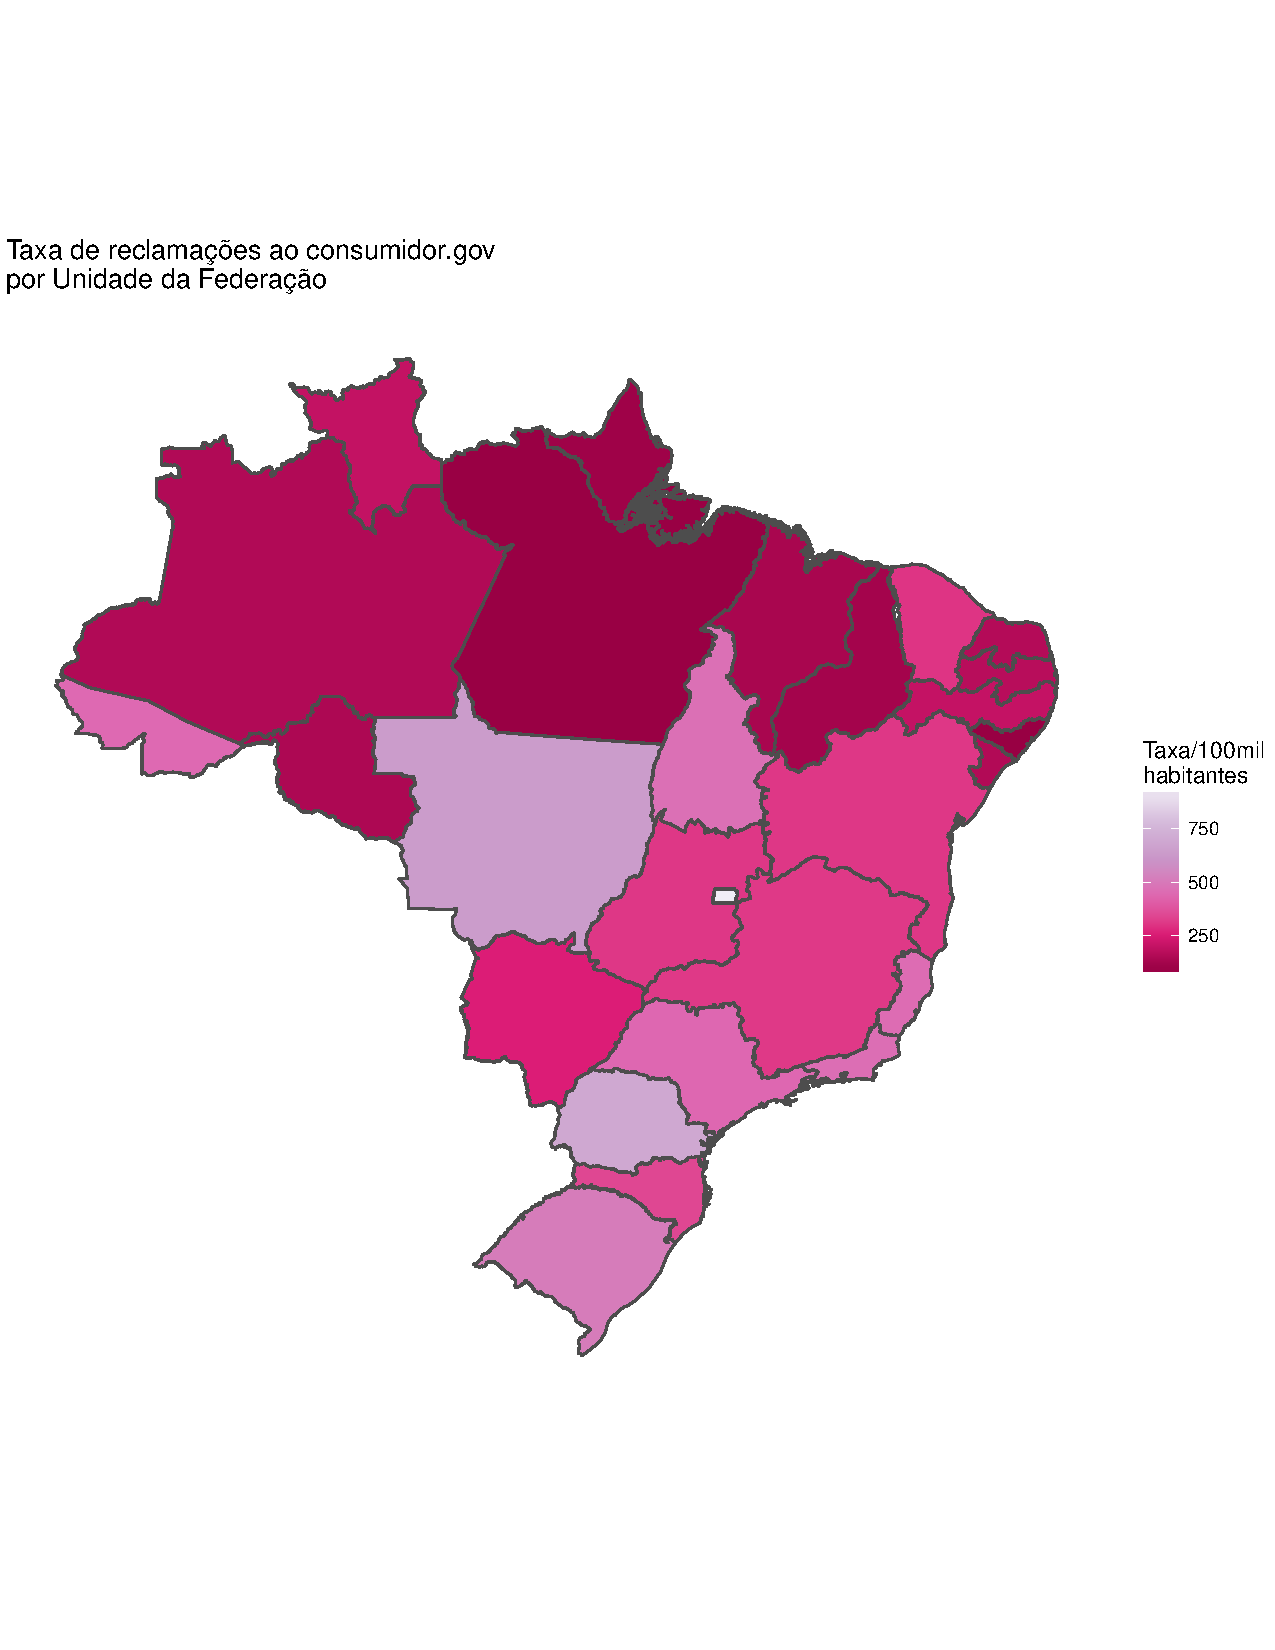
\includegraphics{imgs/mapa_senacon.pdf}
\caption{Taxa de reclamações ao consumidor.gov Unidade da
Federação.}\label{senacon_uf}
\end{figure}

Pode-se argumentar que esse fato não é de grande valia para a mensuração
que se estamos fazendo, pois o mapa acima não considera nenhuma medida
de distribuição de renda dentro das unidades da federação. Isso é
relevante, pois sabe-se que a renda é um influenciador importante do
acesso à justiça.

\begin{figure}[htbp]
\centering
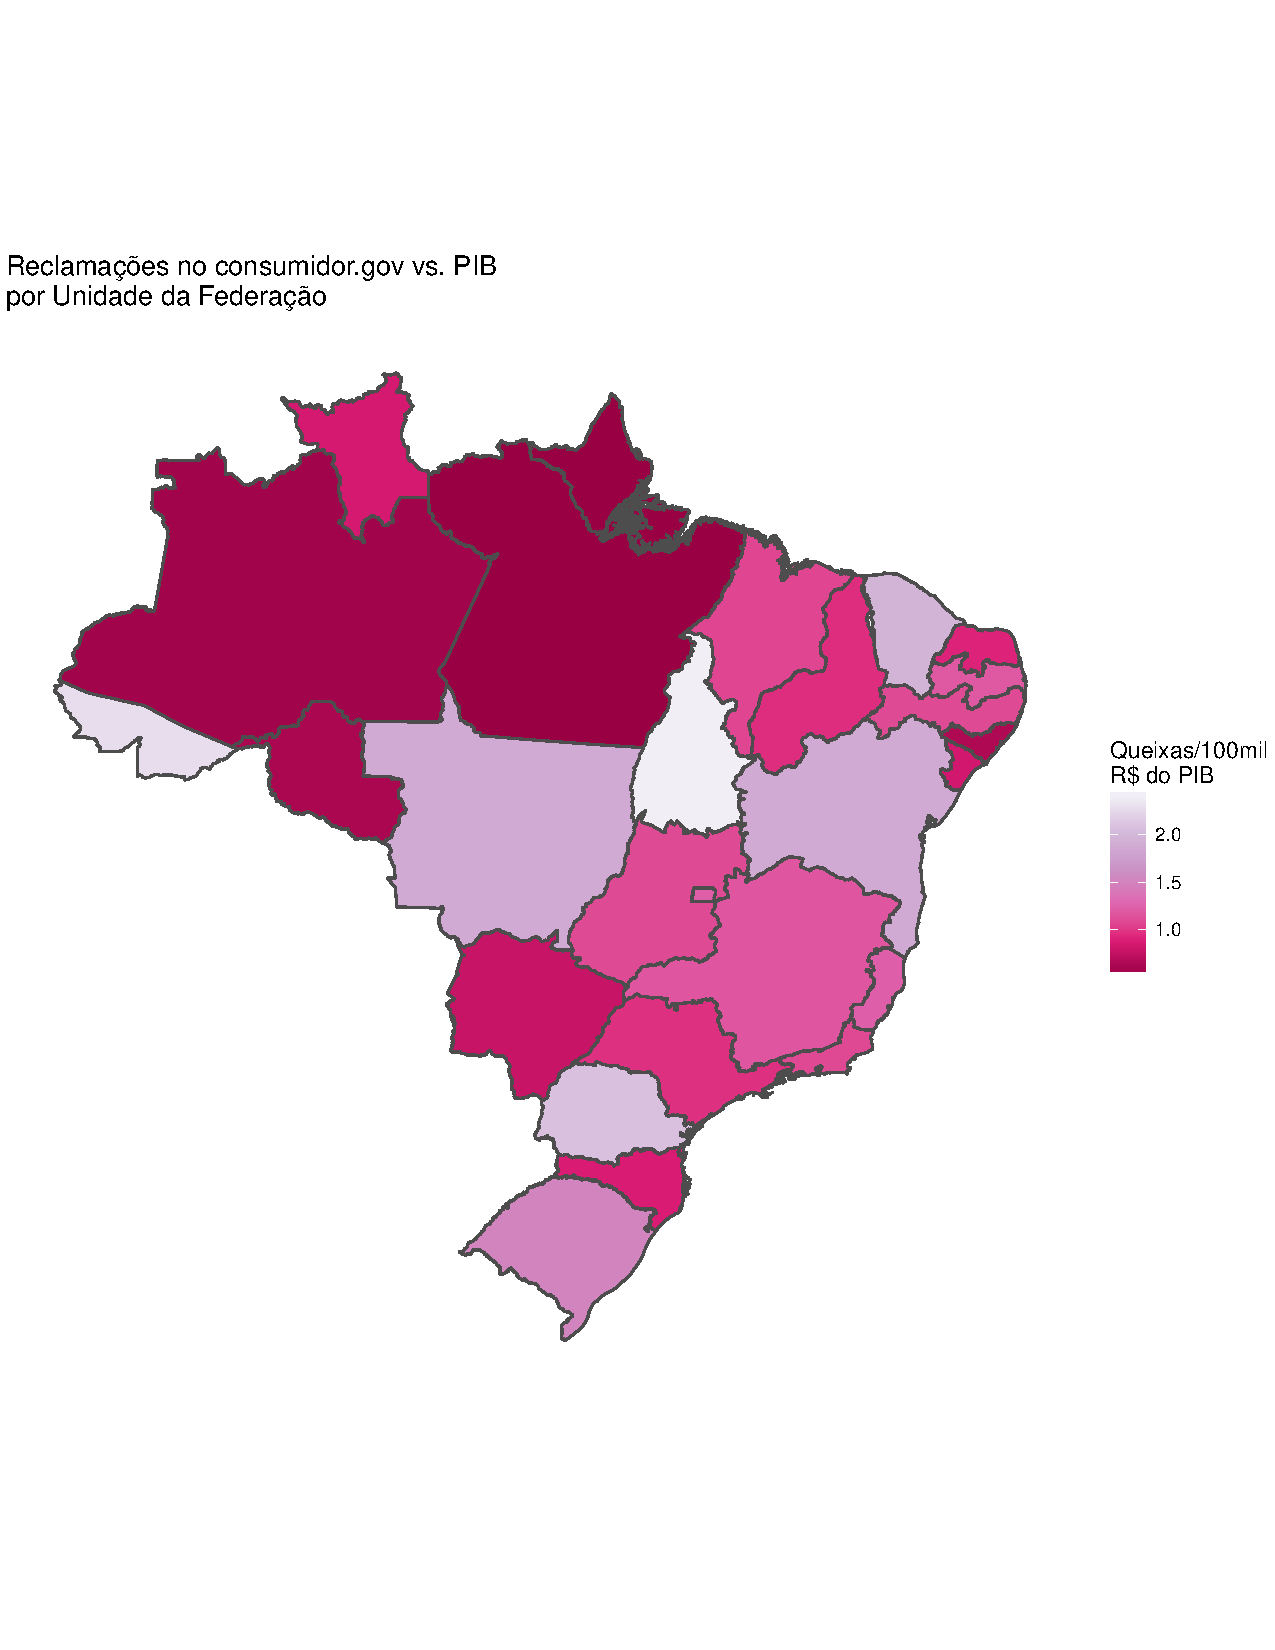
\includegraphics{imgs/senacon_pib.pdf}
\caption{Taxa de reclamações ao consumidor.gov Unidade da
Federação.}\label{senacon_pib}
\end{figure}

Refazendo a análise anterior tomando como referência o Produto Interno
Bruto da unidade da federação, os estados do Nordeste apresentam taxas
próximas às taxas calculadas no Sul e Sudeste, mas com um notável
desnível se mantém na região norte do País. Enquanto a maior parte dos
estados brasileiros apresenta a razão de uma queixa por cada 100 mil
reais do PIB do estado, no Norte essa razão cai pela metade.

Também vale ressaltar que, embora os estados do Norte sistematicamente
acessem menos o consumidor.gov, as taxas do Alagoas e Mato Grosso do Sul
são comparáveis as taxas da região Norte.

\begin{longtable}{lr}
\caption{Reclamações por 100mil reais do PIB separadas por unidade da federação. Fonte: SENACON.} \\
  \hline
Uf & Reclamações Por 100Mil Reais Do Pib \\
  \hline
AL & 0,65 \\
  AM & 0,57 \\
  AP & 0,52 \\
  MS & 0,78 \\
  PA & 0,52 \\
  RO & 0,62 \\
  RR & 0,85 \\
   \hline
\hline
\label{unnamed-chunk-91}
\end{longtable}

Além dos fatores geográficos e econômicos, também desejamos identificar
se fatores temporais influenciam o número de reclamações encaminhadas à
SENACON, a fim de verificar se o uso dessa ferramenta está crescendo,
diminuindo ou estabilizando-se. Desconsiderando variações regionais,
verifica-se que o número de reclamações ao consumidor.gov estão
crescendo.

\begin{figure}[htbp]
\centering
\includegraphics{bookdown_files/figure-latex/unnamed-chunk-92-1.pdf}
\caption{\label{fig:unnamed-chunk-92}Número de reclamações por mês. Fonte:
SENACON.}
\end{figure}

Separando a sequência de consumos mensais por unidades da federação, a
conclusão é a mesma, com poucas exceções. Apenas nos estados do Acre,
Tocantins e Sergipe observa-se uma curva diferente das demais. Nesses
estados o padrão observado está mais próximo de uma reta com picos, no
começo de 2015 no Acre e final de 2016 em Sergipe e Tocantins.

\begin{figure}[htbp]
\centering
\includegraphics{bookdown_files/figure-latex/unnamed-chunk-93-1.pdf}
\caption{\label{fig:unnamed-chunk-93}Número de reclamações por mês em cada
UF. Fonte: SENACON.}
\end{figure}

Como a procura ao site depende apenas dos consumidores, informações
pessoais sobre eles também são importantes para compreender qual tipo de
público está mais suscetível a resolver litígios potenciais usando essa
ferramenta.

As informações sobre os usuários que são disponibilizadas publicamente
pela Senacon são a faixa etária e o sexo e verificam-se padrões nesses
dados. Sobre o sexo pode-se afirmar que o número de mulheres reclamantes
é 18,5\% maior do que o de homens. Já sobre as idades, verifica-se que a
faixa com mais reclamantes corresponde às idades de 21 a 40 anos, sendo
essa observação independente do sexo. Para pessoas com idade superior a
40 anos, a proporção de reclamantes cai conforme a idade avança.

Com relação às idades, verifica-se que a faixa com mais reclamantes
corresponde às idades de 21 a 40 anos, e essa observação vale para os
dois sexos. Para pessoas com idade superior a 40 anos, a proporção de
reclamantes cai conforme a idade avança.

\begin{figure}[htbp]
\centering
\includegraphics{bookdown_files/figure-latex/unnamed-chunk-95-1.pdf}
\caption{\label{fig:unnamed-chunk-95}Perfis dos reclamantes à SENACON com
relação a sexo e idade. Fonte: SENACON.}
\end{figure}

\subsection{Maiores demandados no
consumidor.gov}\label{maiores-demandados-no-consumidor.gov}

Verifica-se uma diferença entre o perfil das demandadas no portal
consumidor.gov e o perfil das demandadas dos tribunais. Por um lado,
similar ao que ocorre nos tribunais, os primeiros da lista de maiores
demandadas do consumidor.gov são empresas de telecomunicações e bancos.
Entretanto, as administradoras de cadastros de inadimplentes possuem
maior representação aqui do que nos tribunais.

\begin{longtable}{lrll}
\caption{30 maiores demandadas da SENACON. Fonte: SENACON.} \\
  \hline
Nome da Empresa ou Grupo & Frequência & Percentual & Percentual Acumulado \\
  \hline
Oi
Telecomunicações & 95643 & 14,1\% & 14,1\% \\
  Vivo & 81654 & 12,0\% & 26,1\% \\
  Claro & 51077 & 7,5\% & 33,6\% \\
  Tim & 48138 & 7,1\% & 40,7\% \\
  Sky & 30098 & 4,4\% & 45,2\% \\
  Bradesco & 28540 & 4,2\% & 49,4\% \\
  Cef & 27370 & 4,0\% & 53,4\% \\
  Itaú & 26571 & 3,9\% & 57,3\% \\
  Serasa Experian & 22069 & 3,3\% & 60,6\% \\
  Boa Vista SPC & 21539 & 3,2\% & 63,7\% \\
  Net & 18621 & 2,7\% & 66,5\% \\
  Santander & 16486 & 2,4\% & 68,9\% \\
  Samsung & 16157 & 2,4\% & 71,3\% \\
  Banco do Brasil & 13813 & 2,0\% & 73,3\% \\
  Casasbahiacom & 12437 & 1,8\% & 75,1\% \\
  Pontofriocom & 11375 & 1,7\% & 76,8\% \\
  Extracom & 10859 & 1,6\% & 78,4\% \\
  Bmg & 9614 & 1,4\% & 79,8\% \\
  Americanascom & 7219 & 1,1\% & 80,9\% \\
  Nextel & 6321 & 0,9\% & 81,8\% \\
  Banco Pan & 5982 & 0,9\% & 82,7\% \\
  Walmartcom & 5705 & 0,8\% & 83,5\% \\
  Tam & 4816 & 0,7\% & 84,3\% \\
  Submarino & 4717 & 0,7\% & 84,9\% \\
  Magazineluizacom & 4263 & 0,6\% & 85,6\% \\
  Carrefour & 4035 & 0,6\% & 86,2\% \\
  Lg & 3836 & 0,6\% & 86,7\% \\
  Ricardoeletro & 3645 & 0,5\% & 87,3\% \\
  Vvar & 3570 & 0,5\% & 87,8\% \\
  Banco
Votorantim & 3025 & 0,4\% & 88,2\% \\
   \hline
\hline
\label{unnamed-chunk-96}
\end{longtable}

\subsection{Eficácia da composição}\label{eficacia-da-composicao}

Nesta seção exploramos a eficácia com que os conflitos apresentados às
demandadas são resolvidos no próprio site. Um ponto bastante relevante
foi o impacto da causa de pedir e da empresa demandada na negociação.

Similar ao realizado nas subseções anteriores, primeiro investigamos os
padrões regionais que incidem sobre as negociações. Globalmente, a
proporção de reclamações resolvidas é de 65.3\%, mas ele varia entre
60.4\%, no Rio de Janeiro e 73\%, em Tocantins.

\begin{figure}[htbp]
\centering
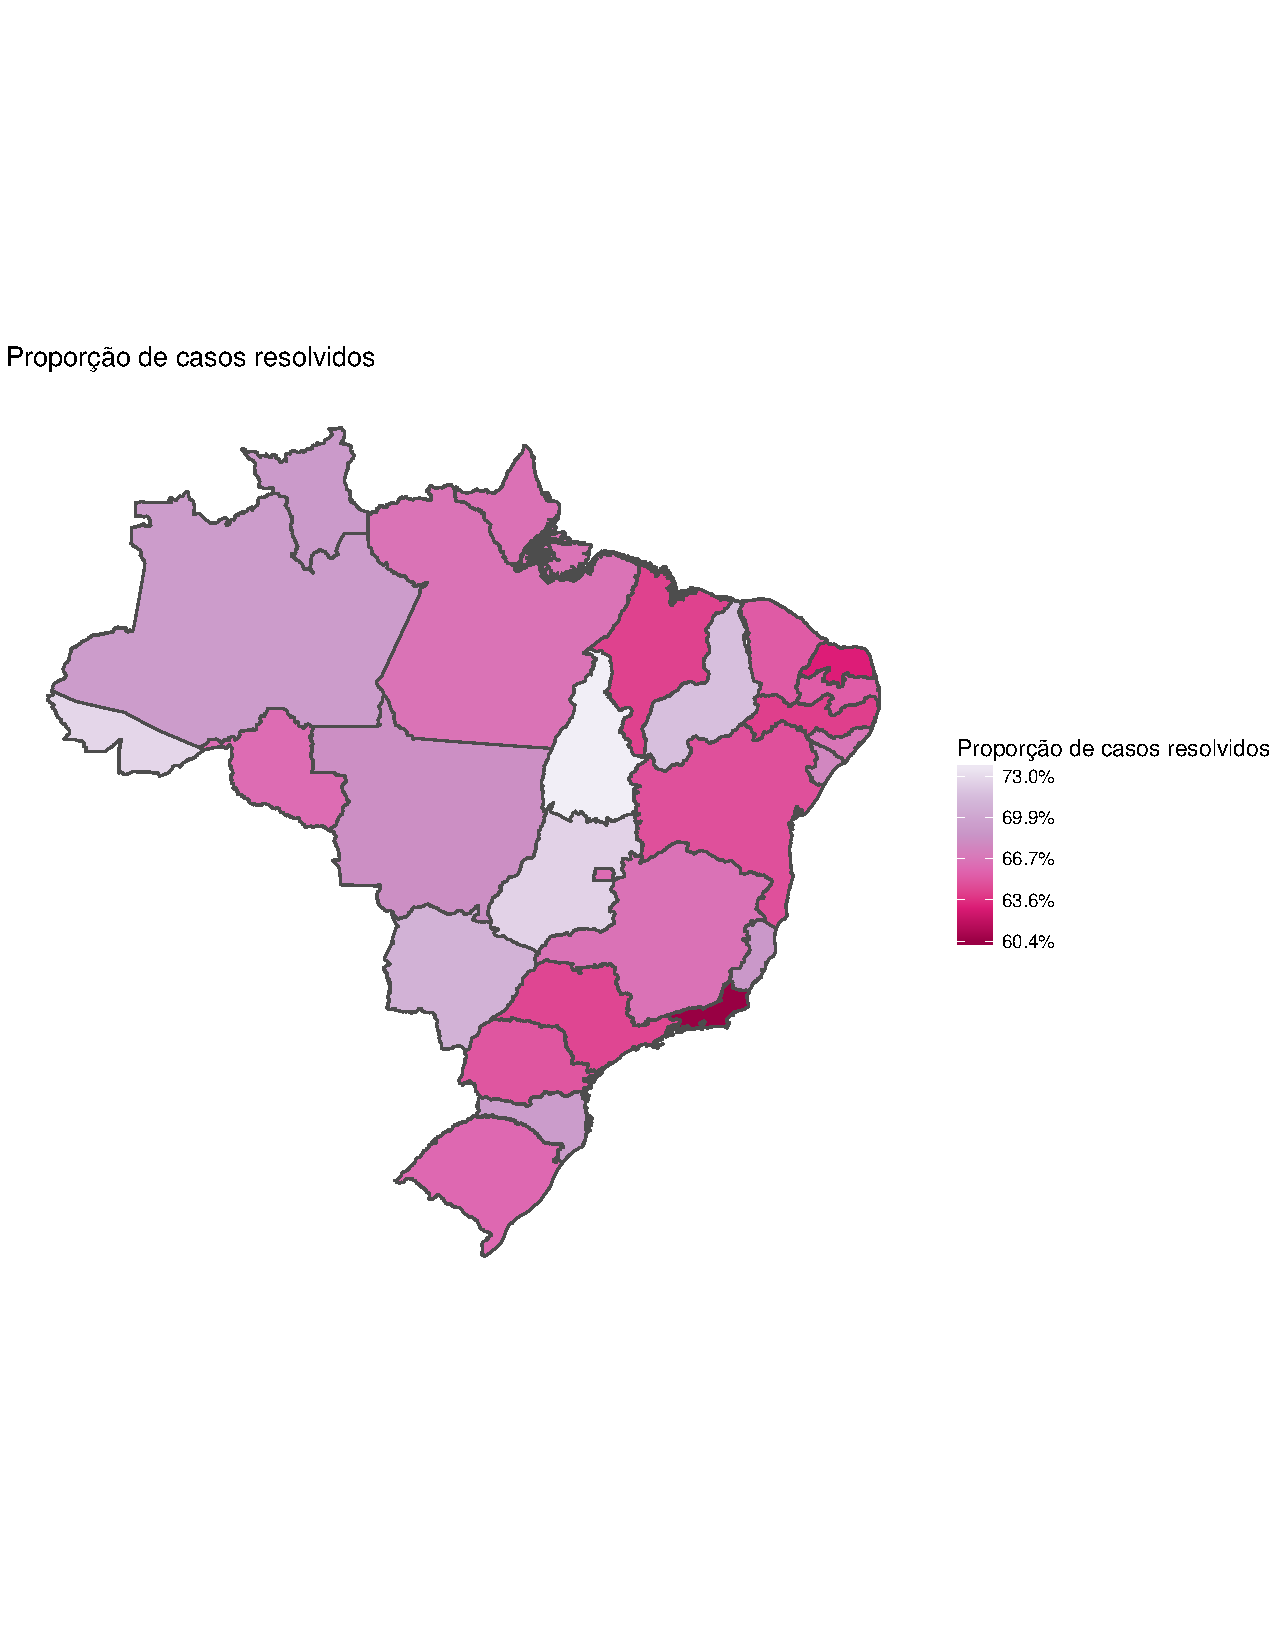
\includegraphics{imgs/senacon_p_uf.pdf}
\caption{Proporção de casos resolvidos, dentre os avaliados pelo
usuários, separados por unidade da federação. Fonte: SENACON.}
\end{figure}

A proporção de casos resolvidos varia mais de acordo com a empresa
demandada do que em função da unidade da federação. Comparando as taxas
de resolução das reclamações por empresa, percebe-se, por exemplo, que
as empresas de telecomunicações têm uma vantagem significativa sobre as
instituições financeiras: a proporção de reclamações resolvidas por
empresas de telecomunicações fica entre 70\% e 80\%, enquanto a mesma
taxa para instituições financeiras fica em torno de 50\%. As empresas
com menor taxa de conversão são as concessionárias de serviços básicos,
que conseguem apenas 25\% de satisfação na avaliação dos usuários.

\begin{figure}[htbp]
\centering
\includegraphics{bookdown_files/figure-latex/unnamed-chunk-98-1.pdf}
\caption{\label{fig:unnamed-chunk-98}Distribuição da proporção de casos
resolvidos, separados por setor econômico. Fonte: SENACON.}
\end{figure}

Essa vantagem se mantém inclusive se compararmos os processos pelos
diferentes assuntos. Tomando apenas as instituições financeiras e
empresas de telefonia e assuntos com mais do que 1000 reclamações, a
média de efetividade de todos os assuntos em empresas de
telecomunicações é 77,1\%, enquanto o mesmo valor para instituições
bancárias é 51\%.

\subsection{Composição Extrajudicial e
Litígios}\label{composicao-extrajudicial-e-litigios}

Embora não fosse possível verificar diretamente se um litigante utilizou
previamente alguma via de composição extrajudicial, pudemos comparar a
quantidade de reclamações com a quantidade de litígios e obter uma cota
superior para a procura por vias de composição extrajudicial. Os
resultados da última subseção sugeriram que, dependendo da magnitude
dessas cotas, é razoável acreditar que se mais demandantes procurassem o
portal consumidor.gov antes de um litígio, menos processos consumeristas
seriam ajuizados.

No Tribunal de Justiça do Rio Grande do Sul, por exemplo, os percentuais
estimados de reclamantes que procuraram vias de composição extrajudicial
são muito pequenos, ao passo que as taxas de eficiência são
razoavelmente altas. Se, para fins de comparação, tomarmos apenas os
processos contra a Oi, Vivo, Claro, Tim, Bradesco e Itaú, teremos o
resultado que segue na tabela abaixo.

\begin{longtable}{lrrr}
\caption{Proporção de casos resolvidos e percentual máximo de litigantes que consultaram o consumidor.gov para 6 empresas. Fonte: SENACON e Tribunal de Justiça do Rio Grande do Sul.} \\
  \hline
Empresa & Número De Processos & Proporção De Casos Resolvidos & \% Que Consultou O Site \\
  \hline
regex\_bradesco & 9244 & 0,49 & 0,07 \\
  regex\_claro & 9483 & 0,78 & 0,27 \\
  regex\_itau & 6757 & 0,54 & 0,08 \\
  regex\_oi & 31909 & 0,59 & 0,18 \\
  regex\_tim & 9076 & 0,71 & 0,13 \\
  regex\_vivo & 9624 & 0,91 & 0,73 \\
   \hline
\hline
\label{contrafactual_senacon}
\end{longtable}

Usando esses números para simular o que aconteceria se todos os
litigantes procurassem o portal da SENACON, os resultados parecem bem
promissores. No que segue, vamos simular alguns cenários com a
finalidade de estimar quantos processos a menos entrariam no judiciário,
caso a composição extrajudicial se efetivasse.

Nas nossas simulações, vamos adotar algumas premissas. Os pontos abaixo
impactam fortemente as nossas estimativas de ganho, por isso em alguns
momentos vamos adotar posições bastante conversadoras. Fazemos isso com
o intuito de produzir estimativas robustas.

As premissas são:

\begin{enumerate}
\def\labelenumi{\arabic{enumi}.}
\tightlist
\item
  Construímos a cota superior para o percentual de consumidores que
  consultam o consumidor.gov atualmente assumindo que todos os casos do
  consumidor.gov se tornaram processos, independente se o usuário
  declarou-se satisfeito.
\item
  Se todos os litigantes tentassem a composição extrajudicial antes de
  litigar, a taxa de satisfação seria a mesma e, nos casos em que o
  litigante estivesse satisfeito, os litígios seriam evitados.
\end{enumerate}

Tomando como exemplo os processos contra a empresa Oi, tem-se que no
máximo 18\% dos demandantes procuraram a SENACON para tentar composições
extrajudiciais, ao passo que 60\% dos reclamantes do site declaram-se
satisfeitos. Pensando nisso, pode-se argumentar que, se num cenário
hipotético todos os litigantes passassem a procurar vias de composição
extrajudicial antes de entrar com os litígios, então o volume processual
consumerista sobre a Oi diminuiria em 82\% \(\times\) 60\% = 49,2\%,
assumindo que as taxas de conversão se mantivessem.

Aplicando o mesmo raciocínio aos dados da tabela
@ref\{contrafactual\_senacon\}, obtém-se os resultados da tabela
@ref\{resultados\_finais\}. O raciocínio para estimar cada ganho foi o
mesmo utilizado no exemplo da Oi, mas aqui ainda consideramos três
cenários

\begin{enumerate}
\def\labelenumi{\arabic{enumi}.}
\tightlist
\item
  \textbf{Pior cenário}: Se todos os processos tivessem passado pela
  SENACON, a taxa de satisfação cairia em 90\%.
\item
  \textbf{Cenário médio}: Se todos os processos tivessem passado pela
  SENACON, a taxa de satisfação cairia em 50\%.
\item
  \textbf{Melhor cenário}: Se todos os processos tivessem passado pela
  SENACON, a taxa de satisfação seria exatamente igual à taxa observada
  hoje.
\end{enumerate}

\begin{longtable}{lrrrrr}
\caption{Proporção de casos resolvidos e percentual máximo de litigantes que consultaram o consumidor.gov para 6 empresas, com estimativas de ganho no cenário em que as litigantes tentam conciliação antes de entrar com o processo. Fonte: SENACON.} \\
  \hline
Empresa & \% De Satisfação & \% Que Consultou O Site & \% Pior Cenário & \% Cenário Médio & \% Melhor Cenário \\
  \hline
regex\_bradesco & 0,49 & 0,07 & 0,05 & 0,23 & 0,46 \\
  regex\_claro & 0,78 & 0,27 & 0,06 & 0,29 & 0,57 \\
  regex\_itau & 0,54 & 0,08 & 0,05 & 0,25 & 0,49 \\
  regex\_oi & 0,59 & 0,18 & 0,05 & 0,24 & 0,49 \\
  regex\_tim & 0,71 & 0,13 & 0,06 & 0,31 & 0,62 \\
  regex\_vivo & 0,91 & 0,73 & 0,02 & 0,12 & 0,24 \\
   \hline
\hline
\label{unnamed-chunk-100}
\end{longtable}

\subsection{Tempos}\label{tempos}

Considerando a discussão da última sessão, fez-se relevante calcular a
celeridade e o número de reclamações efetivamente atendidas por cada
litigante. Avaliar a eficiência do canal de composição extrajudicial da
SENACON também envolve considerar o tempo com o qual as reclamações são
resolvidas.

A média global do tempo de resposta de reclamações é de 6,69 dias.
Entretanto, como os segmentos bancários e de telefonia são usualmente os
mais expressivos na justiça consumerista, vamos nos ater a calcular os
tempos médios para esses segmentos.

Realizando um procedimento similar ao procedimento da última sessão,
tomamos a média dos tempos médios de todos os tempos de processos de
telefonia e bancos separados pelos assuntos, com mais de 1000
observações. Dessa forma, concluímos que os bancos levam, em média 7,04
dias para responder as demandas, enquanto as empresas de
telecomunicações levam, em média 7,35.

\hypertarget{sugestoes-para-aprimoramento-do-sistema}{\chapter{Sugestões
para aprimoramento do
sistema}\label{sugestoes-para-aprimoramento-do-sistema}}

Nesse capítulo, apresentamos uma lista de recomendações com o objetivo
de aprimorar a administração judiciária, posto que tais sugestões não se
limitam apenas à justiça consumerista.

Ressaltamos que as recomendações apresentadas não integram uma única
política pública articulada. A grande maioria pode ser implementada de
maneira isolada, sem depender da implementação das demais.

Esclarecemos também que as medidas apresentadas nem sempre refletem
sugestões efetivas de implementação por parte da ABJ e de seus
associados. O propósito na elaboração da lista foi disponibilizar aos
agentes de governo uma visão sobre diferentes soluções possíveis para o
problema.

Primeiramente, apresentamos um resumo dos principais resultados obtidos
na pesquisa. Os resultados foram organizados de acordo com os objetivos
propostos na introdução.

Em seguida, apresentamos um total de 8 sugestões. A maioria das
propostas são aplicáveis no plano técnico e não temos nenhuma proposta
consolidada de mudança legislativa. Entendemos que tais recomendações
são capazes de provocar uma reflexão aprofundada sobre o problema e
propiciar um melhor entendimento a respeito das soluções que seriam mais
adequadas à nossa realidade.

No final, apresentamos três sugestões de novas pesquisas. O intuito das
sugestões é aprofundar os levantamentos realizados ou investigar outros
temas importantes para o direito do consumidor.

\section{Resumo dos principais resultados da
pesquisa.}\label{resumo-dos-principais-resultados-da-pesquisa.}

\textbf{Os maiores litigantes em ações consumeristas na Justiça
Estadual}. A Tabela \ref{tab:resultAll} mostra os 5 maiores litigantes
em cada Tribunal da pesquisa, acompanhados da estimativa da participação
das empresas dentro do total de processos consumeristas de cada
Tribunal. Bradesco é a única empresa que figura dentre os cinco maiores
litigantes em todos os estados analisados. Outros bancos e empresas de
telecomunicações também aparecem no topo dos maiores litigantes com
frequência.

\begin{longtable}{lrrrr}
\caption{Maiores litigantes em ações consumeristas. Fonte: Elboração própria.} \\
  \hline
Tribunal & Nome da Empresa ou Grupo & Frequência & Percentual & Percentual Acumulado \\
  \hline
TJAM & Manaus
Ambiental & 2162 & 14,6\% & 14,6\% \\
  TJAM & Bradesco & 1291 & 8,7\% & 23,4\% \\
  TJAM & Lider & 1024 & 6,9\% & 30,3\% \\
  TJAM & Itaú & 895 & 6,1\% & 36,4\% \\
  TJAM & Amazonas
Energia & 773 & 5,2\% & 41,6\% \\
  TJBA & Bradesco & 695 & 9,66\% & 9,7\% \\
  TJBA & Itaú & 520 & 7,23\% & 16,9\% \\
  TJBA & Banco
Votorantim & 484 & 6,73\% & 23,6\% \\
  TJBA & Lider & 375 & 5,21\% & 28,8\% \\
  TJBA & Banco Pan & 374 & 5,20\% & 34,0\% \\
  TJDFT & Claro & 4725 & 8,95\% & 9\% \\
  TJDFT & Oi
Telecomunicações & 2544 & 4,82\% & 14\% \\
  TJDFT & Vivo & 2274 & 4,31\% & 18\% \\
  TJDFT & Bradesco & 1963 & 3,72\% & 22\% \\
  TJDFT & Banco do Brasil & 1865 & 3,53\% & 25\% \\
  TJMT & Bradesco & 14459 & 9,98\% & 10\% \\
  TJMT & Claro & 13042 & 9,00\% & 19\% \\
  TJMT & Energisa & 11114 & 7,67\% & 27\% \\
  TJMT & Vivo & 10234 & 7,06\% & 34\% \\
  TJMT & Oi
Telecomunicações & 9723 & 6,71\% & 40\% \\
  TJRJ & Oi
Telecomunicações & 226062 & 12,8\% & 13\% \\
  TJRJ & Itaú & 122621 & 7,0\% & 20\% \\
  TJRJ & Claro & 107584 & 6,1\% & 26\% \\
  TJRJ & Bradesco & 84886 & 4,8\% & 31\% \\
  TJRJ & Light & 79794 & 4,5\% & 35\% \\
  TJRS & Oi
Telecomunicações & 142900 & 13,0\% & 13,0\% \\
  TJRS & Serasa Experian & 96803 & 8,8\% & 21,8\% \\
  TJRS & Itaú & 46323 & 4,2\% & 26,0\% \\
  TJRS & Boa Vista Spc & 45816 & 4,2\% & 30,1\% \\
  TJRS & Bradesco & 40106 & 3,6\% & 33,8\% \\
  TJSP & Itaú & 93263 & 9,28\% & 9,3\% \\
  TJSP & Bradesco & 62701 & 6,24\% & 15,5\% \\
  TJSP & Vivo & 60983 & 6,07\% & 21,6\% \\
  TJSP & Banco
Votorantim & 59517 & 5,92\% & 27,5\% \\
  TJSP & Santander & 39995 & 3,98\% & 31,5\% \\
   \hline
\hline
\label{tab:resultAll}
\end{longtable}

A Figura \ref{fig:acu} mostra a proporção acumulada de processos dos 30
maiores litigantes relativa à totalidade de processos consumeristas. O
gráfico verifica a hipótese inicial da pesquisa de que os trinta maiores
litigantes concentram pelo menos 50\% dos processos. De fato, quatro dos
sete tribunais analisados apresentam proporções acumuladas maiores que
70\%, e cinco tribunais concentram aproximadamente 50\% dos processos
apenas com os 10 maiores litigantes. O tribunal com menor concentração
dos maiores litigantes é o Tribunal de Justiça do Distrito Federal e dos
Territórios (TJDFT), que permanece sua proporção abaixo dos demais
tribunais para todas as quantidades de empresas pontuadas.

\begin{figure}[htbp]
\centering
\includegraphics{bookdown_files/figure-latex/fig:acu-1.pdf}
\caption{(\#fig:fig:acu)Proporção acumulada de processos consumeristas
dos 30 maiores litigantes em cada estado. Fonte: Elboração própria.}
\end{figure}

\textbf{Características dos litigantes e de seus litígios}. A Tabela
\ref{tab:setoresAll} mostra os três setores com maior concentração de
casos em cada Tribunal. Em relação ao perfil dos litigantes, ficou clara
a concentração do setor bancário e setor de telecomunicações. Em relação
ao perfil dos litígios, observamos uma grande concentração de casos de
dano moral e contratos, mas com significativas variações de acordo com
setor e região.

\begin{longtable}{lrrrr}
\caption{Setores dos litigantes em ações consumeristas. Fonte: Elboração própria.} \\
  \hline
Tribunal & Area & Frequência & Percentual & Percentual Acumulado \\
  \hline
TJAM & Instituições
Financeiras & 4159 & 28,1\% & 28,1\% \\
  TJAM & Concessionárias
de serviços
básicos & 2939 & 19,9\% & 48,0\% \\
  TJAM & Telecomunicações & 1997 & 13,5\% & 61,5\% \\
  TJBA & Instituições
Financeiras & 3700 & 51,5\% & 51,5\% \\
  TJBA & Companhias de
seguro & 1141 & 15,9\% & 67,3\% \\
  TJBA & Telecomunicações & 263 & 3,7\% & 71,0\% \\
  TJDFT & Telecomunicações & 13251 & 20,4\% & 20,4\% \\
  TJDFT & Instituições
Financeiras & 9538 & 14,7\% & 35,2\% \\
  TJDFT & Transporte
Aéreo & 3353 & 5,2\% & 40,3\% \\
  TJMT & Instituições
Financeiras & 41367 & 24,9\% & 24,9\% \\
  TJMT & Telecomunicações & 39941 & 24,1\% & 49,0\% \\
  TJMT & Companhias de
seguro & 15305 & 9,2\% & 58,2\% \\
  TJRJ & Telecomunicações & 574943 & 32,7\% & 32,7\% \\
  TJRJ & Instituições
Financeiras & 428275 & 24,3\% & 57,0\% \\
  TJRJ & Concessionárias
de serviços
básicos & 154413 & 8,8\% & 65,8\% \\
  TJRS & Instituições
Financeiras & 308171 & 28,0\% & 28,0\% \\
  TJRS & Telecomunicações & 246293 & 22,4\% & 50,4\% \\
  TJRS & Administradoras
De Cadastro De
Inadimplentes & 183300 & 16,7\% & 67,0\% \\
  TJSP & Instituições
Financeiras & 409940 & 40,3\% & 40,3\% \\
  TJSP & Telecomunicações & 152812 & 15,0\% & 55,3\% \\
  TJSP & Companhias de
seguro & 32278 & 3,2\% & 58,5\% \\
   \hline
\hline
\label{unnamed-chunk-103}
\end{longtable}

\textbf{De que forma os maiores litigantes variam regionalmente}. A
partir da Tabela \ref{tab:resultAll} e as tabelas completas de maiores
litigantes nas respectivas Seções do capítulo de resultados, é
interessante notar que os maiores litigantes mudam de perfil em cada
região. No TJSP e no TJBA, os bancos Itaú e Bradesco aparecem antes das
empresas de telecomunicação. No TJRJ e TJDFT, as empresas Oi, Vivo e
Claro aparecem com destaque. No TJMT e no TJAM, além das empresas de
telecomunicação e bancos, observamos empresas de energia ou seguros
DPVAT. No TJRS, observamos um resultado diferenciado, por conta da
presença de administradoras de cadastros de inadimplentes, como
explicado na Seção de resultados.

Os resultados indicam que existe uma relação entre os tipos de empresas
que aparecem como maiores litigantes e o desenvolvimento econômico da
região. Assim, áreas mais desenvolvidas tendem a concentrar mais casos
envolvendo bancos e, enquanto áreas menos desenvolvidas tendem a
concentrar casos envolvendo fornecedores de serviços essenciais. Para
verificar essa hipótese de maneira aprofundada, sugerimos realizar
estudos locais, como descrito na Seção
\ref{pesquisas-realizadas-localmente}

\textbf{Características dos meios alternativos ao litígio}. Nessa
pesquisa, o principal meio alternativo ao litígio estudado teve como
base os dados fornecidos em formato aberto pela Senacon, contendo
informações detalhadas do sistema consumidor.gov.br. Os resultados são
positivamente surpreendentes. Por exemplo, identificamos uma taxa de
resolução de conflitos média de 76\% na área de telecomunicações. Além
disso, o tempo médio global de resolução de conflitos é de uma semana.

\textbf{Como as grandes empresas do setor privado veem o problema das
ações consumeristas}. Com base nas entrevistas, pode-se afirmar que as
empresas têm grandes preocupações com ações consumeristas e acreditam
que buscar soluções alternativas ao litígio é a melhor forma de
solucionar o problema. As empresas também apresentaram preocupações com
relação a possível existência de advogados oportunistas e indústrias da
gratuidade e do dano moral. No entanto, nenhum desses resultados foi
testado empiricamente e continuam como hipóteses para futuras pesquisas.

\textbf{Soluções administrativas para lidar com os casos pendentes e
reduzir a entrada de novos casos no judiciário}. A partir das reuniões
realizadas no decorrer da pesquisa, acredita-se que aumentar incentivos
ao acordo no judiciário não terá efeitos significativos sobre os casos
já pendentes. No entanto isso não passa de uma hipótese e, por isso,
sugerimos a realização de uma pesquisa aprofundada sobre a Semana da
Conciliação na Seção @ref(experimento-com-semana-da-conciliação) testar
esse efeito. Para reduzir a entrada de novos casos, a solução principal
foi proposta na próxima Seção.

\section{Integração do judiciário com o
consumidor.gov.br}\label{integracao-do-judiciario-com-o-consumidor.gov.br}

A presente solução é a mais importante da pesquisa. Além de ser a
solução com maior impacto esperado para evitar novos processos, é
tecnicamente viável, de baixo custo e seu impacto é mensurável.

As análises da base de dados do consumidor.gov.br revelaram que as
reclamações pré processuais, além de rápidas são eficientes, com uma
taxa de resolução de problemas de quase 80\% na área de telecomunicações
e de mais de 50\% para problemas com bancos.

Nossa proposta para desafogar os tribunais e evitar novos pleitos é
criar um fluxo para direcionar as demandas ao consumidor.gov.br antes de
levar o problema a juízo. Seguindo esse trânsito, garantimos que houve
uma tentativa de comunicação entre as partes através do
consumidor.gov.br, sem gerar demandas adicionais ao judiciário e ao
consumidor.

A Figura \ref{fig:senacon} mostra o fluxo simplificado de como funciona
a solução. Dado um conflito, o consumidor pode, entre outras
alternativas, entrar com uma reclamação no consumidor.gov.br ou iniciar
uma petição inicial eletrônica. No formulário de cadastro da petição
inicial, será adicionado um campo para inserir o código identificador de
reclamações prévias do mesmo tema no consumidor.gov.br. Se o autor da
ação deixar esse campo em branco, uma reclamação é gerada paralelamente
a fim de viabilizar uma tentativa de conciliação extrajudicial. Se o
conflito for resolvido pelo consumidor.gov.br, o processo é encerrado.
Em caso de o conflito não ser resolvido em um prazo fixo, o procedimento
no consumidor.gov.br é encerrado e o processo judicial corre
normalmente.

\begin{figure}[htbp]
\centering
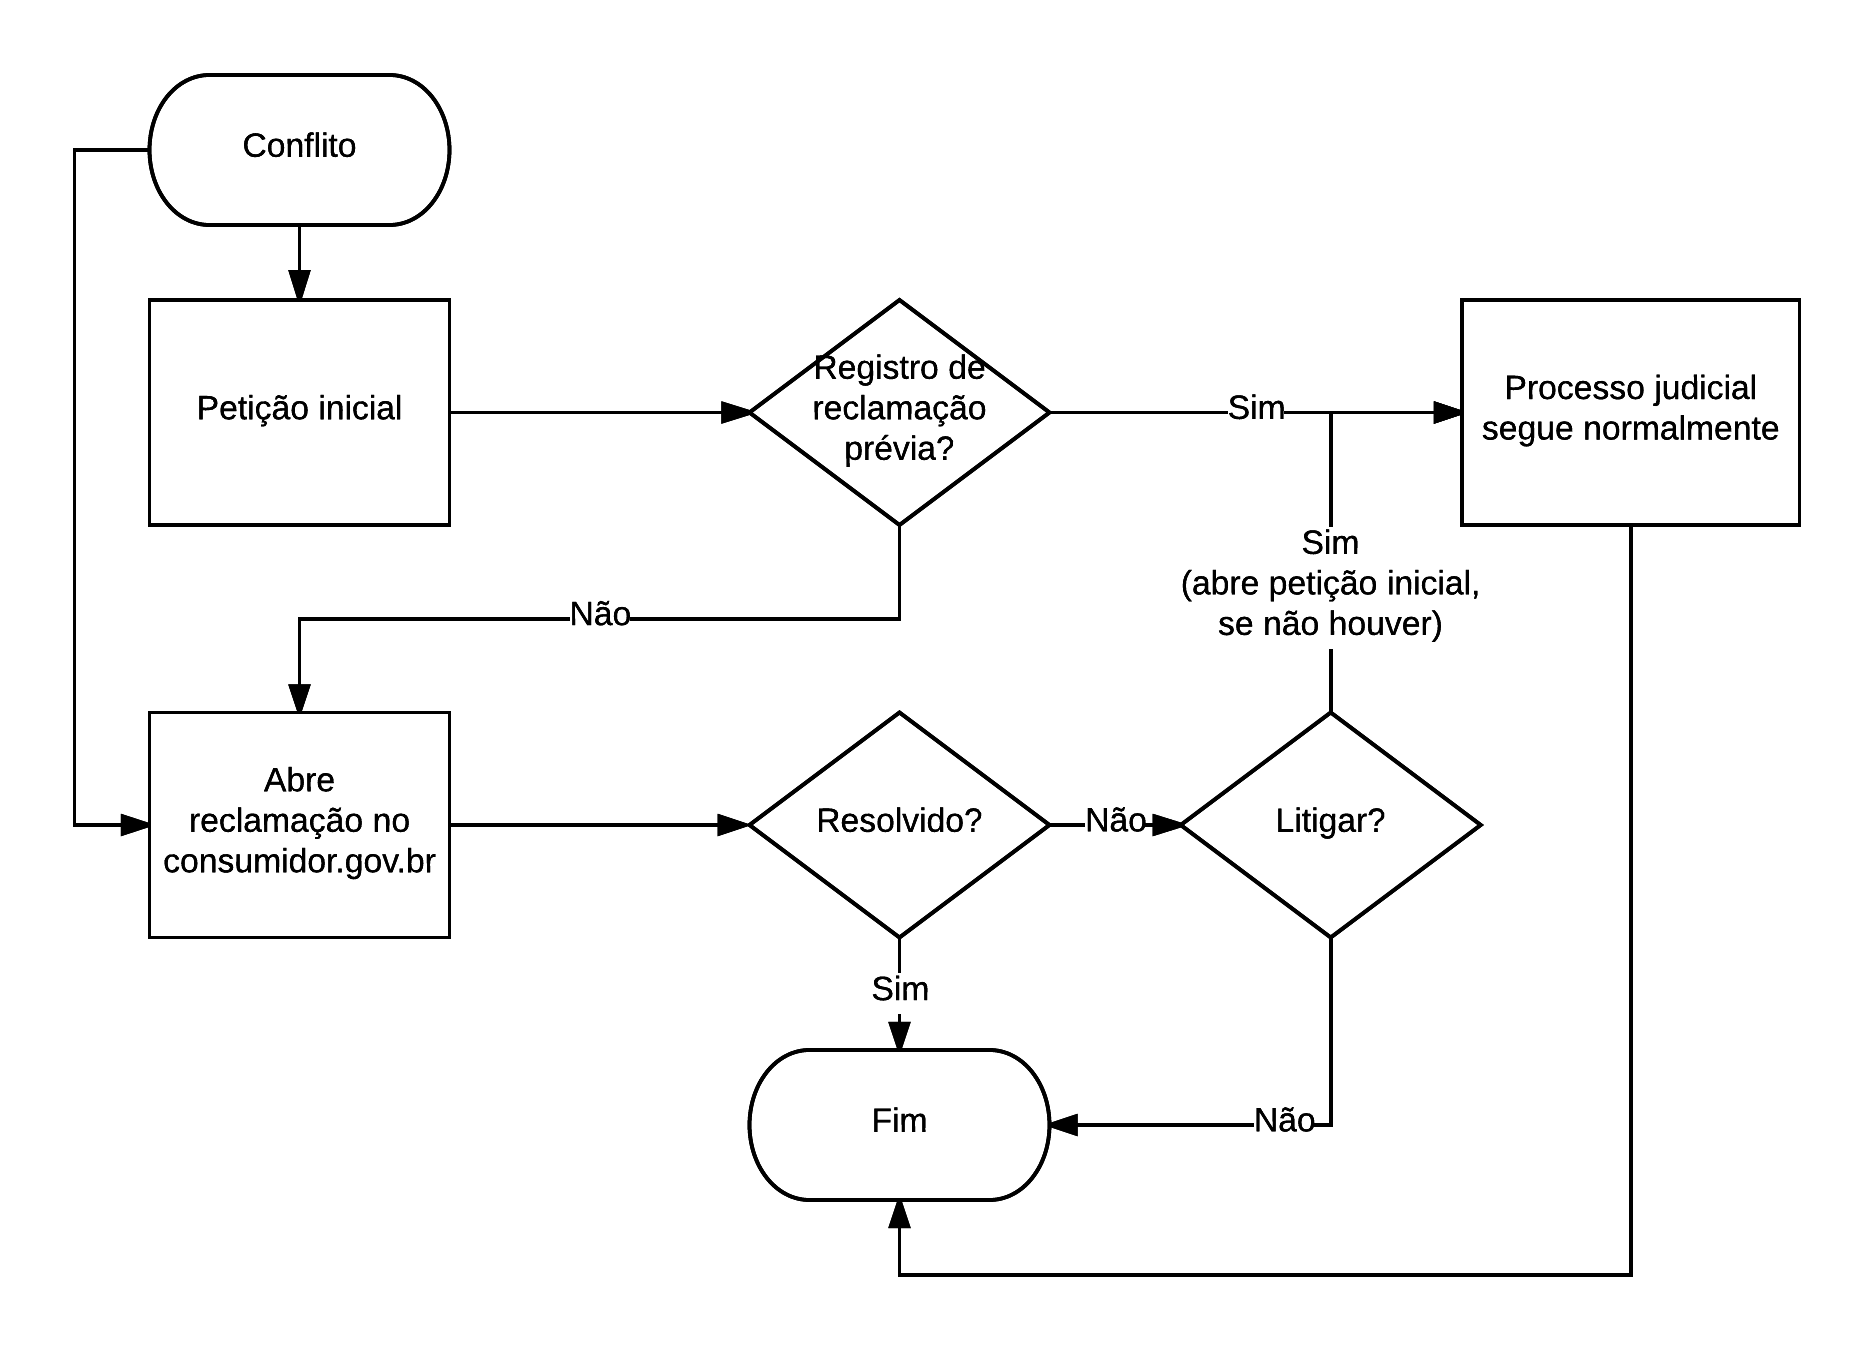
\includegraphics{imgs/senacon.png}
\caption{Fluxo de integração genérico.}\label{senacon}
\end{figure}

Essa solução possui as seguintes vantagens:

\begin{enumerate}
\def\labelenumi{\arabic{enumi}.}
\tightlist
\item
  Obriga a empresa a atender o reclamante rapidamente.
\item
  Provavelmente não atrasa o andamento do processo, visto que i) os
  procedimentos correm em paralelo, ii) o prazo de atendimento no
  consumidor.gov.br é curto e iii) os diálogos realizados através da
  plataforma auxiliam na tomada de decisão no processo judicial.
\item
  Evita a entrada de ações desnecessárias, ou seja, que podem ser
  resolvidas extrajudicialmente.
\item
  Desincentiva a entrada de litigantes e advogados oportunistas, uma vez
  que o consumidor.gov.br terá registro das discussões travadas entre
  reclamante e empresa.
\item
  Auxilia na documentação das reclamações, em razão do consumidor.gov.br
  possuir modelos de dados mais adequados para registrar informações
  sobre as queixas do que os sistemas dos tribunais.
\item
  Não afeta negativamente o acesso à justiça, já que o processo judicial
  é distribuído de qualquer forma.
\end{enumerate}

Uma possível desvantagem da solução é que para alguns ela pode
burocratizar a abertura do processo judicial. Por exemplo, se uma pessoa
busca uma composição amigável via SAC ou ferramentas como o Reclame
Aqui, ela repetirá o procedimento no consumidor.gov.br após entrar com
uma ação. Ainda assim, considerando a velocidade de atendimento do
canal, essa barreira tem impacto negativo negligenciável frente às
vantagens obtidas.

A implementação não precisa ser feita em nível nacional em sua primeira
versão. Inclusive, o ideal é que a solução seja implementada
gradativamente e de forma planejada, garantindo i) o atendimento de um
cronograma de implementação e ii) uma avaliação do impacto utilizando
índices de atendimento da demanda.

Existem duas formas principais de aplicar a solução proposta de forma
gradativa.

A primeira é selecionar algumas comarcas de interesse para adicionar o
campo do formulário conectado com o consumidor.gov.br. A solução tem uma
facilidade adicional, já que em casos consumeristas o endereço
considerado pode ser o do autor do processo (Lei 8.078/1990, art.101,
I). Dessa forma, selecionar uma comarca de interesse tende a representar
o perfil dos autores do processo, ao invés dos réus.

A segunda estratégia é iniciar os testes com alguns dos maiores
litigantes identificados na pesquisa. O argumento para isso é que, como
o volume de conflitos é muito grande, algumas empresas podem não estar
preparadas para atender a demanda imediata.

O potencial dessa proposta para redução da litigiosidade é muito
relevante, uma vez que afeta todos os peticionamentos eletrônicos. Essa
também é uma forma adequada de aumentar a eficiência do judiciário, pois
somente irão a juízo os casos que comprovadamente não forem resolvidos
extrajudicialmente.

\section{Criação de ferramentas de
monitoramento}\label{criacao-de-ferramentas-de-monitoramento}

A presente pesquisa auxiliou na identificação de eventos anômalos na
litigiosidade. O maior exemplo disso foi o pico repentino na entrada de
ações contra o Serasa no TJRS. Tais eventos podem acontecer de maneira
localizada e nem sempre são perceptíveis nos grandes números.

No entanto, relatórios técnicos são ineficazes para identificar e
controlar eventos anômalos dinamicamente. A solução adequada nesse caso
é a criação de \emph{dashboards} interativos e ferramentas de alerta.
Idealmente, o CNJ e os Tribunais precisam ter uma ferramenta desse tipo
nas Secretarias de Planejamento Estratégico (SEPLAN) e nas
Corregedorias.

O Núcleo de Monitoramento de Perfis de Demandas da Corregedoria Geral da
Justiça de São Paulo (NUMOPEDE) foi criado a partir do expediente CPA nº
2016/163905 e tem como objetivo monitorar demandas que, pelas suas
características, impactam de forma substancial na organização dos
serviços judiciais. A análise das demandas a partir do seu perfil pode
se justificar, entre outros casos, por picos de distribuição em curto
espaço de tempo, pelas características do litígio ou dos litigantes.

A proposta do grupo é racionalizar os trabalhos cartorários e coibir a
utilização predatória da justiça. Para isso, monitoram a evolução de
casos novos de forma contínua, segregando por i) classe e assunto; ii)
comarca; iii) partes e advogados responsáveis. Dessa forma, é possível
identificar picos temporais de distribuições de processos em
determinadas localidades ou envolvendo empresas específicas, gerando
alertas para agilizar na tomada de decisões estratégicas.

A sugestão para o CNJ sobre esse tema é entrar em contato com a equipe
responsável pelo NUMOPEDE e definir passos para a implementação de uma
ferramenta de visualização nacional para identificação de eventos
anômalos. A ferramenta pode funcionar como uma aba adicional do recente
módulo de produtividade mensal do CNJ.

\section{Metodologia de cálculo de volumes processuais por
assunto}\label{metodologia-de-calculo-de-volumes-processuais-por-assunto}

Compreender o perfil das demandas é indispensável para a gestão
eficiente dos Tribunais. Uma forma natural de identificar esses perfis é
classificando os casos em tipos, que são grupos de processos com
características comuns.

Atualmente, a forma mais direta de identificar tipos de processos
judiciais é utilizando os chamados \emph{assuntos processuais}. Os
assuntos relacionam-se com as matérias discutidas em cada caso. Por
exemplo, um caso cível de indenização por dano moral poderia ter um
assunto ``Indenização por dano moral'', enquanto um processo falimentar
de uma empresa em Recuperação Judicial poderia ser classificado como
``Convocação de Recuperação Judicial em Falência''.

Nesse contexto, um importante passo foi dado com a Resolução 46/2007 do
CNJ\footnote{\url{http://www.cnj.jus.br/images/stories/docs_cnj/resolucao/rescnj_46.pdf}.
  Acesso em 26/06/2017.}, que criou as TPUs. As TPUs são uma
documentação oficial de todas as classes, assuntos e movimentações dos
processos. As TPUs foram implantadas em todas as Justiças, o que
facilita a realização de análises que comparam diferentes tribunais.

As TPUs são estruturadas em formato de árvore. Isso significa que temos
assuntos genéricos e assuntos específicos, sendo que o assunto
específico é um ``filho'' do assunto genérico. As TPUs podem ter até
seis níveis hierárquicos de assuntos.

O problema enfrentado atualmente é que muitas vezes os processos são
classificados com assuntos genéricos. Assim, ao contar todos os
processos de determinado tema, podemos contar casos a menos por conta de
problemas de classificação.

Subestimar do volume real de processos de um certo tipo configura a
\textbf{cifra oculta}, que é dada pela quantidade de processos de um
assunto classificados em assuntos genéricos.

A cifra oculta pode ser estimada usando técnicas estatísticas
apropriadas. Para isso, no entanto, é necessário fazer algumas
suposições ou utilizar conhecimentos de especialistas sobre o tema. No
capítulo de metodologia apresentamos uma solução replicável para
resolver o problema.

A solução apresentada depende de algumas suposições, mas poderia ser
rapidamente implementada em sistemas e relatórios gerenciais. Um caso
importante é o Módulo de Produtividade Mensal do CNJ, que poderia
apresentar estimativas de volume processual para todos os assuntos.

\section{Utilização da métrica IADR para avaliação de
impactos}\label{utilizacao-da-metrica-iadr-para-avaliacao-de-impactos-das-medidas}

Toda medida adotada para aprimoramento da administração judiciária
precisa ser avaliada no plano prático, ainda que faça sentido
teoricamente. Sem avaliação, não é possível aferir eficácia e, por
conseguinte, é difícil propor melhorias.

Na metodologia também apresentamos uma métrica chamada IADR: Índice de
Atendimento à Demanda Relativo, que pode ser visto como uma
generalização da taxa de congestionamento e do Índice de Atendimento à
Demanda (IAD) para estudar a litigiosidade de um tribunal.

A proposta nesse caso é utilizar o IADR para avaliar o impacto de
mudanças. O peso relativo dos casos pendentes a ser utilizado no cálculo
dependerá de decisões estratégicas e será objeto de futuras pesquisas.

Caso a primeira proposta dessa pesquisa seja implementada, seria
possível calcular a evolução mensal do IADR em processos consumeristas.
Nesse caso, a implementação gradativa em diferentes comarcas/estados
permitiria a comparação do IADR usando técnicas como \emph{differences
in differences} \citep{bertrand2004much}, que resultam em estimativas
razoáveis sobre os efeitos das políticas.

\section{Utilização de modelos de classificação de
partes}\label{utilizacao-de-modelos-de-classificacao-de-partes}

Um dos maiores desafios metodológicos enfrentados durante a realização
da presente pesquisa foi a limpeza e classificação das partes nos
processos.

Parte das bases vieram com nomes de empresas acompanhados dos documentos
(CPF ou CNPJ). Em tese, a tarefa de contagem a partir dos CNPJs seria
trivial. No entanto, os diversos problemas de documentação presentes
nessas bases nos forçaram a utilizar os nomes das empresas como base em
todos os casos.

Classificar as empresas a partir dos nomes também não é trivial, pois os
nomes podem aparecer de formas distintas. Em alguns casos, nem mesmo
seres humanos são capazes de distinguir, por exemplo, se uma parte é
pessoa jurídica ou física, olhando apenas para o nome.

No decorrer dos trabalhos, testamos vários modelos de classificação das
partes. Os modelos partiram de expressões regulares e criação de
\emph{white lists}\footnote{Uma \emph{white list} é uma lista de nomes
  que certamente ou quase certamente indicam como classificar o nome da
  parte. Essa lista inclui nomes de empresas conhecidas, como Bradesco,
  Itaú etc.}, que foram se tornando mais sofisticados com a aplicação de
técnicas como regressão LASSO \citep{friedman2001elements} em
\emph{sacolas de palavras}\footnote{\emph{Bag of words} ou sacola de
  palavras é uma maneira de organizar textos a partir da contagem de
  palavras em documentos. Uma característica importante da sacola de
  palavras é que ela não considera a ordem em que as palavras aparecem.
  Assim, por exemplo, Itaú Unibanco e Unibanco Itaú são equivalentes.}.
No final, acabamos considerando um conjunto de expressões regulares,
pela simplicidade e estabilidade dos resultados.

A grande vantagem do trabalho realizado é que a classificação é
replicável. Isso significa que uma nova pesquisa na área de maiores
litigantes poderia utilizar o mesmo código para realizar a classificação
das empresas. Além disso, o código é aberto e pode ser testado e
melhorado.

A solução final foi implementada num pacote escrito em R chamado
\texttt{tidyML}\footnote{Acesso em
  \url{https://github.com/abjur/tidyML}. No momento de elaboração desse
  texto, o tidyML ainda não estava finalizado.}. Nossa sugestão nesse
caso é que o pacote seja testado e melhorado com sugestões de outros
pesquisadores. Dessa forma, será possível reclassificar os nomes de
empresas em todos os Tribunais de maneira unificada, facilitando muito
na realização de levantamentos futuros.

\section{Sistema de Classificação de Empresas e
Incorporações}\label{sistema-de-classificacao-de-empresas-e-incorporacoes}

Para a realização desse projeto, foi necessário pesquisar o histórico
das empresas e suas incorporações. Isso foi feito, dentre muitos outros
casos, para o Itaú e Unibanco, que nos dias de hoje são parte da mesma
corporação.

Um problema dessa tarefa é a necessidade de tomadas de decisão
arbitrárias. Por exemplo, decidimos manter separadas as empresas Via
Varejo e GPA, que até o momento desta redação eram controladas pelo
grupo Casino.

Para o atendimento dos princípios da transparência e reprodutibilidade,
é importante que uma tabela de-para oficial das empresas e suas
incorporações seja disponibilizada publicamente. Essa tabela deve ser
dinâmica pois as incorporações acontecem a todo momento.

Nossa sugestão é que o Sistema de Classificação de Empresas e
Incorporações (SCEI) seja uma ferramenta similar às Tabelas Processuais
Unificadas do CNJ. As empresas devem ser classificadas em formato de
árvore, acompanhadas de seus códigos, que nesse caso serão os CNPJs.
Especialistas cadastrados no SCEI poderiam propor mudanças nessa
classificação ao longo do tempo.

Na ABJ sempre nos esforçamos para manter os códigos utilizados para
realização das análises disponíveis. Caso a sugestão da tabela seja
implementada, os códigos desenvolvidos para essa pesquisa podem auxiliar
na criação da versão inicial das tabelas.

\section{Experimento com semana da
conciliação}\label{experimento-com-semana-da-conciliacao}

O CNJ promove anualmente a Semana Nacional da Conciliação. Trata-se de
uma campanha de mobilização na qual todos os Tribunais Brasileiros
concentram seus esforços, durante uma semana, na obtenção do maior
número possível de composições amigáveis.

Além de ser uma forma de reduzir o volume processual, a semana da
conciliação é uma oportunidade muito interessante para conduzir
experimentos. Tais experimentos poderiam ser utilizados para mensurar o
efeito do incentivo à conciliação, buscando estabelecer os limites desse
efeito.

Uma forma de conduzir o experimento é selecionando aleatoriamente
processos elegíveis ou não na semana de conciliação. Dessa forma seria
possível isolar o efeito do incentivo à conciliação, sem prejuízo ao
curso natural do processo. Estudos recentes sugerem que é possível
atingir o mesmo objetivo sem a aplicação completa de aleatorização:
\citep{Fossaluza2015} discute o tema da alocação intencional na condução
de experimentos. Com a técnica de alocação sequencial, é possível testar
hipóteses com amostras menores.

Um resultado interessante desses experimentos é a possibilidade de
testar a hipótese de que adicionar cláusulas para incentivar conciliação
é efetivo. Em estudos observacionais, essa inferência causal não seria
possível, pois o efeito estaria confundido \citep{pearl2009causality}.

\section{API pública para extração de
processos}\label{api-publica-para-extracao-de-processos}

Existem inúmeras ferramentas públicas e privadas para busca e
recuperação de processos. Os sistemas são eficazes, mas são todos
voltados para a busca de informações individuais. Se uma pessoa tiver o
número identificador, ela achará informações do processo. Se precisar
uma lista de processos, poderá utilizar ferramentas de busca.

Cientistas de dados, no entanto, precisam ter a possibilidade de
exportar os dados completos ou algum recorte da população para
planilhas. Existem muitos exemplos de páginas úteis para cientistas de
dados, como IpeaData, Datasus, IBGE, entre outros.

Também é possível utilizar \emph{Application Programming Interfaces}
(APIs) para obter dados de \emph{tweets}, publicações no Facebook, entre
outros. O importante é notar que os sistemas voltados para análise de
dados são em sua maioria voltados para extração de informações de muitos
indivíduos. Os dados são organizados para análise e não para consulta
individual. Muitas vezes é necessário limpar a base, mas isso faz parte
do fluxo da ciência de dados \citep{wickham2016r}.

Na área do direito, o pesquisador fica numa situação complicada, pois
precisa de dados da população ou de uma amostra, com linhas e colunas,
numa planilha padronizada. No entanto, tudo o que consegue encontrar são
documentos individuais, listagens de processos e arquivos em formato
fechado, como o \emph{Portable Document Format} (PDF).

Muitas vezes os dados estão disponíveis em páginas web mas é muito
demorado buscar todos os casos que precisamos manualmente ou através de
ofícios. Por isso, é usual construir \emph{web scrapers}, que são robôs
que baixam as páginas automaticamente e depois as tranformam em dados
estruturados.

Atualmente, a utilização \emph{web scrapers} é indispensável em estudo
jurimétricos. As pesquisas realizadas pela ABJ foram fortemente
influenciadas por essas ferramentas.

Contudo, são raros os profissionais que dominam esse conhecimento. A ABJ
disponibiliza abertamente todo seu aparato técnico \footnote{Disponíveis
  nos links:\url{https://github.com/abjur} (códigos genéricos da ABJ),
  \url{https://github.com/courtsbr} (web scrapers), e
  \url{https://github.com/decryptr} (ferramentas para quebrar CAPTCHAs).},
mas as ferramentas não são capazes de resolver todos os problemas. Além
disso, os sistemas dos Tribunais colocam impedimentos técnicos de
acesso, dificultando a execução de pesquisas que poderiam ser benéficas
para os próprios Tribunais.

Há muitos exemplos em que simplesmente não é possível obter as
informações que necessitamos. Em muitos casos a única forma de acessar
os dados é a partir da Lei de Acesso à Informação. Apesar da LAI ser um
grande avanço, utilizá-la para todas as demandas é ineficiente pois
congestiona os setores administrativos e técnicos dos Tribunais.

A solução mais eficaz para o problema de acesso aos dados envolve
modificar os sites dos Tribunais, permitindo extrações de dados e
disponibilizar APIs que permitam os pesquisadores de buscar as
informações públicas de maneira segura e organizada.

Essas ferramentas são simples de construir para entidades como os
Tribunais, que geralmente têm equipes de Tecnologia da Informação de
altíssima qualidade. A solução não causaria impactos negativos nos
sistemas; pelo contrário: ao permitir que os dados sejam baixados de
forma programática, é possível controlar o volume de dados transferido
por unidade de tempo, evitando que os servidores fiquem sobrecarregados.

A ABJ tem atuado em campanhas de abertura de dados do judiciário,
construindo ferramentas, organizando eventos, ministrando cursos e
fazendo contatos políticos. A Associação se coloca disponível para
auxiliar na definição de modelos de dados e formas de utilização das
APIs. Acreditamos que num futuro próximo o Brasil será referência
mundial na abertura de dados do Judiciário.

\section{Sugestões de novas
pesquisas}\label{sugestoes-de-novas-pesquisas}

É próprio e esperado da pesquisa apresentada que o levantamento de dados
provoque novos questionamentos a respeito de problemas até então
insuspeitos. Cada resposta traz consigo novas perguntas.

Ao elaborar os relatórios procuramos incluir algumas questões não
diretamente ligadas ao problema da justiça consumerista, mas que
intuíamos àquela altura estarem ligadas a outras questões sensíveis ao
tema.

Os resultados apresentados, apesar de não serem conclusivos, são
suficientemente significativos para que as autoridades responsáveis se
preocupem em investigá-los com maior profundidade nas próximas
pesquisas.

A recomendação final é, portanto, a realização de novas pesquisas sobre
pontos importantes que afetam a administração do judiciário. Sem
prejuízo de outras temáticas, os quatro tópicos abaixo nos pareceram
importantes.

\section{Pesquisas realizadas
localmente}\label{pesquisas-realizadas-localmente}

Reduzir a cobertura nacional da pesquisa, e aumentar a quantidade de
observações dentro de cada região. Em todas as pesquisas empíricas no
direito, fica claro que locais com diferentes estruturas administrativas
e diferentes culturas influenciam muito nas características dos
processos \citep{abj2015}. Uma alternativa para solucionar esse problema
é realizar uma amostra aleatória de varas e estudá-las de forma
aprofundada, buscando conhecer e controlar a variabilidade. No entanto,
é difícil controlar essa variabilidade a nível nacional, pois cada
visita às varas pode incorrer em custos e tempo dispendido. Por esse
motivo, uma sugestão é a realização de pesquisas locais, voltadas ao
estudo das unidades federativas. Pesquisas como essa ainda seriam
custosas pelo elevado número de comarcas, mas produziriam resultados
mais consistentes.

\section{Pesquisas envolvendo gratuidade
judiciária}\label{pesquisas-envolvendo-gratuidade-judiciaria}

Como observamos na presente pesquisa, um dos processos mais recorrentes
do direito do consumidor são os casos que envolvem danos morais, um
assunto processual que tem a intuição de estar associado a uma
indústria. Por um lado, isso poderia ser explicado pela existência de
magistrados com tendência a favorecer o autor da ação, ou seja, que
arbitram valores de indenização altos o suficiente para convencer
pessoas a litigar. Em outras ocasiões, é possível ajuizar litígios que
desfavorecem a requerida em prol da requerente, além do simples intuito
de indenizar um dano sofrido.

Um tópico relevante nesse contexto é a gratuidade judiciária, que tem
fundamento no princípio constitucional da inafastabilidade do poder
judiciário (CF, art. 5º, XXXV). A gratuidade também se encontra guarida
na oferta constitucional de assistência judiciária integral e gratuita
àqueles que comprovarem insuficiência de recursos (CF, art. 5º, LXXIV).

O objetivo geral dessa pesquisa é comparar os perfis de processos com e
sem o benefício da justiça gratuita.

As principais métricas de comparação inicialmente propostas foram
listadas abaixo.

\begin{enumerate}
\def\labelenumi{\arabic{enumi}.}
\tightlist
\item
  Tempo entre a distribuição e sentença ou arquivamento do processo.
\item
  Proporção de decisões favoráveis/parcialmente favoráveis.
\item
  Valor de indenização do processo e proporção de acordos.
\item
  Características socioeconômicas dos autores.
\end{enumerate}

Esse estudo pode ser usado para testar se mudanças administrativas nas
regras para concessão da gratuidade teriam efeito na litigiosidade. Essa
pesquisa teria de lidar obrigatoriamente com o princípio do acesso à
justiça, a fim de evitar que uma decisão de política pública seja tomada
unicamente para favorecer a eficiência do judiciário.

\section{Relação entre desenvolvimento e
litigiosidade}\label{relacao-entre-desenvolvimento-e-litigiosidade}

Em 2013 a ABJ organizou seu terceiro Seminário de Jurimetria, onde foi
discutida a relação entre litigiosidade e desenvolvimento. Essa pesquisa
teve como proposta alertar a sociedade de que a litigiosidade é
positivamente associada ao crescimento da população e, por isso,
poderíamos estar mensurando o efeito de ações para barrar a entrada
massiva de novos casos de maneira ineficiente.

A litigiosidade pode ser definida como o número de casos novos por cem
mil habitantes. Já o desenvolvimento pode ser representado por diversas
variáveis, dentre elas o Índice de Desenvolvimento Humano (IDH). A
Figura \ref{fig:litig} mostra um gráfico de dispersão entre essas duas
quantidades, baseando-se nos dados do PNUD (Programa das Nações Unidas
para o Desenvolvimento) para o IDH em 2010 e o RJN para o número de
casos novos por cem mil habitantes em 2015. A correlação observada nesse
caso é de 77\%.

\begin{figure}[htbp]
\centering
\includegraphics{bookdown_files/figure-latex/litig-1.pdf}
\caption{\label{fig:litig}Gráfico de dispersão do IDH-Médio estadual e
quantidade de casos novos por cem mil habitantes. Fonte: Justiça em
Números e PNUD.}
\end{figure}

No entanto, sabemos que correlação não implica em causalidade. Existem
várias explicações possíveis para essas duas variáveis estarem
associadas. Assim, pode ser que um estado receba um incremento na sua
renda per capita sem necessariamente aumentar a litigiosidade.

Nesse contexto, seria interessante realizar uma investigação mais
aprofundada do problema, buscando aferir uma relação causal entre
desenvolvimento e litigiosidade. Uma alternativa para isso seria ligar
bases de dados de processos com bases de dados de trabalhadores, como a
RAIS (Relação Anual de Informações Sociais). Dessa forma, seria possível
investigar se choques positivos na renda das pessoas aumentariam a
probabilidade de entrada na justiça.

Se verificada, a relação causal entre desenvolvimento e litigiosidade
seria útil não só para predizer a demanda futura de processos, mas
também a definir estratégias direcionadas para redução de litígios.

\chapter{Apêndice}\label{apendice}

\section{Códigos utilizados para análise das bases de
dados}\label{codigos-utilizados-para-analise-das-bases-de-dados}

\subsection{Produto 2}\label{produto-2}

\begin{enumerate}
\def\labelenumi{\arabic{enumi}.}
\tightlist
\item
  \href{https://github.com/abjur/cnjML}{Scripts de análise de dados
  feitos em R}.
\item
  \href{https://github.com/abjur/tidyML}{Scripts para arrumar dados dos
  tribunais}.
\item
  \href{https://github.com/abjur/tidyPJ}{Scripts para arrumar nomes das
  empresas}.
\item
  \href{https://github.com/abjur/tpur}{Pacote em R utilizado para
  armazenas as TPUs do CNJ}.
\item
  \href{https://github.com/abjur/tpur}{Pacote em R utilizado para criar
  a \emph{whitelist} do TJSP e estimar volumes processuais}.
\item
  \href{https://github.com/courtsbr/esaj}{Scripts de web scraping de
  tribunais do sistema SAJ}.
\item
  \href{https://github.com/courtsbr/tjsp}{Scripts de web scraping de
  diversas páginas do TJSP}.
\item
  \href{https://github.com/decryptr/}{Modelos para quebrar CAPTCHAs}.
\end{enumerate}

\subsection{Estudo sobre teses da USP}\label{estudo-sobre-teses-da-usp}

\begin{enumerate}
\def\labelenumi{\arabic{enumi}.}
\tightlist
\item
  \href{https://github.com/abjur/esaj}{Pacote em R utilizado para
  download dos acórdãos}.
\item
  \href{https://www.dropbox.com/s/kkqlghd5cv10u99/d_ementas_2014.rda?dl=0}{Base
  de dados sobre acórdãos utilizada}.
\item
  \href{https://github.com/abjur/teses.usp}{Pacote em R utilizado para
  download das teses da USP}.
\item
  \href{https://github.com/jtrecenti/teses.usp/raw/master/data/teses_usp.rda}{Base
  de dados de teses da USP}.
\end{enumerate}

\section{Eixos de investigação cortados no decorrer da
pesquisa}\label{eixos-de-investigacao-cortados-no-decorrer-da-pesquisa}

Os seguintes eixos de investigação foram deixados de lado no decorrer da
pesquisa por serem muito complexos de executar e/ou por apresentarem
pouco potencial de resolver problemas de administração judiciária. Ainda
assim, optamos por manter os eixos, pois outros pesquisadores podem
enxergar oportunidades não identificadas pela ABJ durante a execução do
projeto.

\subsection{Incidentes de demandas
repetitivas}\label{incidentes-de-demandas-repetitivas}

Outra importante ferramenta instituída pelo novo CPC para redução dos
processos em trâmite no Poder Judiciário é o Incidente de Resolução de
Demandas Repetitivas (IRDR), cujo procedimento é regulado pelo artigo
976 e seguintes do novo diploma processual.

O IRDR é cabível quando houver, simultaneamente, duas condições: i)
efetiva repetição de processos que contenham controvérsia sobre a mesma
questão unicamente de direito, tanto material quanto processual; e ii)
risco de ofensa à isonomia e à segurança jurídica.

Isso significa que deve haver aspectos fáticos repetitivos nos diversos
casos analisados. Como, por exemplo, em casos nos quais as partes tenham
realizado o mesmo tipo de atividade negocial e agora discutem com o
Fisco a incidência de Imposto, ou nos quais as partes pretendem a
devolução de valores em razão de planos econômicos instituídos pelo país
no início dos anos 1990.

A instauração do incidente pode ser pedida pelo juiz ou relator, pelas
partes da demanda, pela Defensoria Publíca ou Ministério Público. Quando
o Ministério Público não pedir a instauração do incidente, deverá
funcionar como fiscal da Lei.

O IRDR é julgado pelo órgão do tribunal responsável pela uniformização
da jurisprudência. Admitido o incidente pelo relator, os processos
classificados no grupo correspondente são suspensos. Uma vez julgado o
incidente, a tese jurídica será aplicada conforme o art. 985, I e II:

\begin{quote}
``I - a todos os processos individuais ou coletivos que versem sobre
idêntica questão de direito e que tramitem na área de jurisdição do
respectivo tribunal, inclusive àqueles que tramitem nos juizados
especiais do respectivo Estado ou região; II - aos casos futuros que
versem idêntica questão de direito e que venham a tramitar no território
de competência do tribunal, salvo revisão na forma do art. 986''.
\end{quote}

Do julgamento do mérito do incidente caberá recurso extraordinário ou
especial. O recurso tem efeito suspensivo e a repercussão geral do
recurso extraordinário será presumida. A tese jurídica adotada pelo
Supremo Tribunal Federal (STF) ou pelo Superior Tribunal de Justiça
(STJ) será aplicada no território nacional a todos os processos
individuais ou coletivos que versem sobre idêntica questão de direito.

Por se tratar de um instituto inédito e com pouco tempo de vigência, o
IRDR tem sido pouco utilizado. Pela dificuldade em se identificar o que
deve ser considerado como ``questão unicamente de direito'', é incerto o
efeito de tais medidas.

A única hipótese em relação ao IRDR é que, pelo fato deste tratar de
questões unicamente de direito, este dispositivo do CPC não influencia
os processos que envolvem direito do consumidor de forma significativa.
A hipótese será avaliada a partir de um conjunto de suposições bem
definidas e um modelo de simulação.

O IRDR era um tema potencialmente interessante no início da pesquisa.
Estudar sua aplicação é uma forma de avaliar os impactos do novo CPC no
direito do consumidor. Soluções envolvendo o IRDR também poderiam ajudar
a decidir processos em bloco sem reduzir a segurança jurídica,
aumentando significativamente a eficiência dos tribunais.

Infelizmente, em todas as entrevistas o tema ficou em segundo plano. É
grande a descrença em aplicações práticas do IRDR. E é pequena a fatia
dos problemas do consumidor que ele ataca. Para ser efetivo, o IRDR
precisaria de uma tecnologia de identificação e agrupamento de processos
que ainda não existe em nenhum tribunal. Além disso, existem poucos
casos disponíveis para análise.

Concluímos que o IRDR precisa de tempo para maturar e tornar-se passivo
de análise quantitativa. Por isso, o eixo de investigação foi descartado
na presente pesquisa.

\subsection{Otimização da fila de
trabalho}\label{otimizacao-da-fila-de-trabalho}

A redação original do art. 12 do novo CPC previa, de maneira sucinta,
que os juízes e os tribunais deveriam observar a ordem cronológica de
conclusão para proferir sentenças e acórdãos. No mesmo sentido, a
redação original do art. 153 determinava que o escrivão ou chefe de
secretaria observasse a ordem cronológica de recebimento para publicação
e efetivação dos pronunciamentos judiciais.

Sensível aos problemas que essa determinação poderia trazer para o
funcionamento das varas judiciais e tribunais, o legislador editou a Lei
n.º 13.256/2016, que acrescentou a palavra ``preferencialmente'' aos
artigos 12, Caput, e 153 do CPC:

\begin{quote}
``Art. 12. Os juízes e os tribunais atenderão, preferencialmente, à
ordem cronológica de conclusão para proferir sentença ou acórdão.''

``Art. 153. O escrivão ou o chefe de secretaria atenderá,
preferencialmente, à ordem cronológica de recebimento para publicação e
efetivação dos pronunciamentos judiciais.''
\end{quote}

A partir das modificações perpetradas pela Lei n.º 13.256/2016, os
magistrados, escrivães ou chefes de secretaria não mais estão obrigados
a observar a ordem cronológica de tramitação dos processos. Por isso,
foram estabelecidas exceções à essa regra no parágrafo 2º do
dispositivo.

Dessa forma, tem-se o seguinte:

\begin{itemize}
\tightlist
\item
  O magistrado não está obrigado a seguir a ordem cronológica dos
  processos para proferir sentença ou acórdão, devendo segui-la
  preferencialmente, desde que possível.
\item
  Há exceções legais que determinam que um processo seja julgado antes
  de outros, independentemente de sua ordem cronológica.
\end{itemize}

A liberdade na forma de atuação do juiz nesse sentido pode ser vista
como positiva, pois dessa forma é possível delimitar a ordem que melhor
atenda às necessidades de cada vara. Na prática, no entanto, isso
implica na descentralização da administração das varas, em que cada juiz
administra o cartório de forma arbitrária. Esse problema, somado à
conhecida falta de mecanismos de comunicação entre os juízes, gera uma
sensação de caos na administração da justiça.

Uma forma possível de solucionar esse problema seria através da
otimização da fila de trabalho dentro do cartório. Isso seria realizado
através de um modelo que ordenaria os trabalhos a serem realizados em
cada dia, considerando todos os agentes do cartório.

A hipótese para esse tema é a de que existem formas de ordenar as
tarefas dentro de um cartório capaz de i) minimizar o número de ações a
serem tomadas, através de ações e blocos de processos, ii) reduzir o
tempo médio entre a distribuição e a sentença do processo e iii) manter
constante ou reduzir a taxa de recorribilidade.

Os resultados para esse tema são simulações, baseadas em dados reais de
movimentações processuais e utilização de modelos similares aos
descritos em \citet{Fossaluza2015}. A mensuração da importância envolve,
entre outras características, a complexidade processual. Portanto, a
implementação deve levar em conta métodos para mensuração de
complexidade.

A ideia de otimizar filas de trabalho já nasceu problemática. O tema
surgiu de dentro do Laboratório de Jurimetria e baseia-se na suposição
de que a ordenação de tarefas dentro de uma vara é ineficiente. Um
algoritmo de otimização poderia ser usado para agrupar processos
similares ou tarefas repetidas dentro de processos distintos, eliminando
retrabalho da vara.

Nas entrevistas, observamos que o tribunal já possui diversos modelos de
documentos e ritos bem definidos. Novos padrões para fluxo de trabalho
das varas seria útil apenas em comarcas com menor volume processual. A
solução também apresenta dificuldades de implementação, pois precisa ser
integrado aos sistemas existentes e poderiam exigir treinamento.

\subsection{Incentivos para litigar}\label{incentivos-para-litigar}

Segundo \citet{CNJ2015}, os processos mais recorrentes do direito do
consumidor são os que envolvem danos morais, sendo este um assunto
processual que tem a intuição de estar associado a uma ``indústria''.
Esse fato poderia ser explicado por conta de juízes que arbitram valores
de indenização altos o suficiente, instigando pessoas a litigar. Em
outras ocasiões, é possível ajuizar litígios que desfavorecem a
requerida em prol da requerente, além do simples intuito de indenizar um
dano sofrido.

Esse é argumento particularmente plausível no caso dos JECs, por conta
da inexistência das custas processuais e sucumbência \citep{Athos2015}.
Se desconsiderarmos o custo de litigar por conta do tempo dispendido
para iniciar e acompanhar a ação, mesmo quando a probabilidade de
sucesso é baixa, litigar é um ato vantajoso para o autor, mesmo que este
não tenha razão.

Outro tópico relevante nesse contexto é a gratuidade judiciária, que tem
fundamento no princípio constitucional da inafastabilidade do poder
judiciário (CF, art. 5º, XXXV). A gratuidade também se encontra guarida
na oferta constitucional de assistência judiciária integral e gratuita
àqueles que comprovarem insuficiência de recursos (CF, art. 5º, LXXIV).

O novo CPC derrogou (revogou parcialmente) as disposições da Lei
1.060/1950 e passou a também regular a gratuidade da justiça, que
compreende: i) taxas e custas judiciais; ii) selos postais; iii)
despesas com publicações na imprensa oficial; iv) indenização devida à
testemunha pelo dia não trabalhado; v) despesas com realizações de
exames de DNA e outros considerados essenciais; vi) honorários de
advogados, peritos, remuneração do intérprete ou tradutor; vii) custas
para elaboração de memórias de cálculo, quando exigidas; viii) depósitos
para interposição de recursos, propositura de ação e prática de outros
atos inerentes ao exercício do contraditório e da ampla defesa; ix)
emolumentos devidos a notários ou registradores necessários para
efetivação de decisão judicial ou regular processamento da demanda
(CPC/2015, art. 98, § 1º).

A concessão da gratuidade da justiça não afasta a responsabilidade do
beneficiário pelas despesas processuais e pelos honorários advocatícios
decorrentes de sua sucumbência. Nesse caso, as obrigações do
beneficiário ficarão sob condição suspensiva de exigibilidade e somente
poderão ser executadas se, nos 5 anos subsequentes ao trânsito em
julgado da decisão que as certificou, o credor demonstrar que deixou de
existir a situação de insuficiência do beneficiário.

O momento de concessão da gratuidade da justiça, que pode ocorrer em
relação a algum ou a todos os atos processuais, e que pode consistir na
redução percentual dos valores é regulado pelo art. 99 do novo CPC.

O dispositivo supramencionado prevê, em seu \emph{Caput}, que a
gratuidade pode ser pedida na petição inicial, na contestação, na
petição para ingresso do terceiro ou em recurso. Mas também pode ser
requerida em momento ulterior, por simples petição, desde que a condição
de insuficiência seja superveniente à primeira manifestação da parte. Na
prática, a justiça gratuita pode ser pedida em qualquer momento do
processo.

A possibilidade de o magistrado indeferir o pedido de justiça gratuita,
tema que é o cerne deste tópico, também é tratada no art. 99 do novo
CPC. Trata-se de questão sensível.

O § 3º do art. 99 determina que ``presume-se verdadeira a alegação de
insuficiência deduzida exclusivamente por pessoa natural''. Por sua vez,
o art. 99, §2º, prevê que o magistrado somente poderá indeferir o pedido
se houver nos autos elementos que evidenciem a falta dos pressupostos
para a concessão de gratuidade. E antes de indeferir o pedido, o
magistrado deve possibilitar que a parte comprove o preenchimento dos
requisitos.

Dessa forma, a balança pende para o lado da concessão da justiça
gratuita para as pessoas naturais, na medida em que: i) há uma presunção
de insuficiência por mera declaração; ii) essa presunção somente pode
ser afastada caso o magistrado verifique a existência de elementos que
demonstrem que o réu não possui insuficiência, o que normalmente ocorre
apenas naqueles casos extremos; iii) ainda que o magistrado afaste a
presunção, deve dar à parte a possibilidade de provar que preenche os
requisitos de insuficiência.

Na prática, o que ocorre é que grande parte dos magistrados concedem a
justiça gratuita sem maiores reflexões ou averiguações, exceto quando a
situação de riqueza da parte é muito evidente. Se aceita, a gratuidade
judiciária implica em incentivos similares para litigar quando
comparados aos JECs.

Por outro lado, também precisamos considerar o acesso à justiça para
equacionar os incentivos para litigar de forma adequada. Note que, se
colocarmos um custo de litigar altíssimo, teríamos um judiciário livre
de ações, mas uma sociedade sem acesso à justiça. Mas, se colocarmos um
custo de litigar igual à zero, teríamos amplo acesso à justiça, mas uma
baixa qualidade na prestação jurisdicional.

Também podemos considerar que o custo de litigar varia conforme o poder
econômico do consumidor. Com efeito, duas pessoas envolvidas em
conflitos similares, mas com poderes aquisitivos distintos possuem
incentivos diferentes para entrar com ações judiciais.

Portanto, o fenômeno da litigiosidade em ações consumeristas por parte
do consumidor pode ser estudado a partir de um modelo econométrico que
busca maximizar a eficiência do judiciário. Esse tópico é amplamente
estudado por uma área da jurimetria denominada ``viés de seleção em
decisões judiciais'' \citep{priest1984selection}.

As hipóteses sobre esse tema são:

\begin{enumerate}
\def\labelenumi{\arabic{enumi}.}
\tightlist
\item
  A inexistência de custas processuais e sucumbência na primeira
  instância dos JECs impacta positivamente na entrada de ações
  consumeristas.
\item
  A legislação atual sobre gratuidade judiciária impacta positivamente
  na entrada de ações consumeristas.
\end{enumerate}

Os resultados dessa pesquisa podem influenciar proposições tais como:

\begin{enumerate}
\def\labelenumi{\arabic{enumi}.}
\tightlist
\item
  Metodologias concretas de mensuração do acesso à justiça, com base em
  suposições e critérios bem definidos.
\item
  Alterações na legislação para inclusão de valores ótimos de
  sucumbência e/ou custas processuais, buscando balancear o acesso à
  justiça e a prestação jurisdicional eficiente.
\end{enumerate}

Juízes e empresários têm diferentes hipóteses sobre o valor da taxa de
conversão de conflitos em litígios relacionados ao consumidor, o que
leva a diferentes percepções sobre a influência de fenômenos como a
gratuidade judiciária, as custas processuais nos JECs e a indústria do
dano moral no volume de ações.

\subsection{Motivações para o cometimento de
ilícitos}\label{motivacoes-para-o-cometimento-de-ilicitos}

Neste eixo de investigação temos interesse em estudar as causas de
litigar associadas às empresas. Em particular, desejamos compreender as
motivações por trás do cometimento de ilícitos.

A motivação por trás da elaboração deste eixo reside na suposição de que
uma empresa funciona como agente racional e maximizador de lucro. Dessa
suposição seguem as hipóteses:

\begin{enumerate}
\def\labelenumi{\arabic{enumi}.}
\tightlist
\item
  Se, para uma determinada empresa, o custo associado a administração de
  um litígio for menor que o custo empregado para evitar um ato ilícito,
  então a decisão escolhida pela empresa será cometer o ilícito.
\item
  Uma redução no número de atos ilícitos cometidos acarreta uma
  diminuição do número de litígios.
\end{enumerate}

Utilizando as duas hipóteses, concluímos que se for economicamente
viável pra uma empresa cometer um ato ilícito, então o número de
litígios aumentará. Por outro lado, neste cenário é possível mitigar os
riscos de ilicitudes tornando economicamente inviável o cometimento de
uma infração através de multas ou sanções.

Com esse raciocínio em mente, nossas investigações se concentrarão em
aproximar as condições de contorno à tomada de decisões jurídicas da
administração de uma empresa. Assim, verificaremos se existem meios para
desincentivar o cometimento de atos ilícitos em instituições para as
quais vale a hipótese 1.

Como possíveis resultados, temos a elaboração de propostas para leis,
multas ou sanções que tornem economicamente inviável o cometimento
frequente de ilícitos. Esses dispositivos podem ser operacionalizados em
função do valor médio de indenização ou dano médio causado ao
consumidor.

Esse tema dividiu opiniões nas reuniões. O cometimento de ilícitos é o
insumo dos conflitos entre empresa e consumidor. Na analogia da
torneira, entender as motivações para o cometimento de ilícitos é o
mesmo que estudar o encanamento por trás da torneira. Infelizmente, não
é possível quebrar a parede para analisar o encanamento -- não podemos
investigar nem relatar publicamente as políticas internas dos maiores
litigantes em ações consumeristas.

As análises para o tema ficariam apenas no plano teórico e os modelos
finais poderiam ser aplicadas no mundo real somente após a coleta de
novos dados. Por isso, resolvemos deixar as análises em segundo plano,
possivelmente em pesquisas futuras.

\subsection{Estratégias de composição
amigável}\label{estrategias-de-composicao-amigavel}

As duas maiores inovações do novo CPC são i) a ênfase atribuída ao dever
de cooperação entre as partes e ii) as aberturas para atuação dos
chamados meios alternativos de solução de litígios.

Dentro do âmbito desta última, encontram-se as estratégias de
conciliação e mediação. Dois pontos são relevantes para compreender como
as estratégias de conciliação e mediação podem ajudar na redução do
número de processos que estão em trâmite perante o Poder Judiciário: a
obrigatoriedade da conciliação ou mediação e as semanas nacionais de
conciliação.

\textbf{Obrigatoriedade do procedimento arbitral}. Tendo por objetivo
fomentar a composição amigável, o novo CPC inovou e estabeleceu que os
Tribunais deverão criar centros judiciários de solução consensual de
conflitos através do art. 165:

\begin{quote}
``Art. 165. Os tribunais criarão centros judiciários de solução
consensual de conflitos, responsáveis pela realização de sessões e
audiências de conciliação e mediação e pelo desenvolvimento de programas
destinados a auxiliar, orientar e estimular a autocomposição''.
\end{quote}

Dessa forma foi instituída a figura do conciliador, que atuará
preferencialmente em casos em que não houver vínculo anterior entre as
partes, e do mediador, que atuará preferencialmente em casos em que
houver vínculo anterior entre as partes. A atuação do conciliador ou do
mediador é obrigatória sempre que houver conciliador ou mediador na
comarca na qual se instaurou a situação litigiosa.

Por sua vez, o CPC estabelece que após verificar que a petição inicial
preenche os requisitos essenciais e não é o caso de improcedência
liminar do pedido, o juiz designará audiência de conciliação ou de
mediação. Em outras palavras, a designação da audiência é obrigatória e
deverá ser designada com no mínimo 30 dias de antecedência, devendo o
réu ser citado com 20 dias de antecedência, como estabelece o art. 334:

\begin{quote}
``Art. 334. Se a petição inicial preencher os requisitos essenciais e
não for o caso de improcedência liminar do pedido, o juiz designará
audiência de conciliação ou de mediação com antecedência mínima de 30
(trinta) dias, devendo ser citado o réu com pelo menos 20 (vinte) dias
de antecedência.''
\end{quote}

Em apenas duas hipóteses a audiência de conciliação ou mediação não é
obrigatória. A primeira é quando as partes manifestam expressamente seu
desinteresse na realização da audiência - o autor na petição inicial e
os réus em até 10 dias antes da realização da audiência. A segunda é
quando o direito que estiver em disputa não admitir autocomposição.

Visando garantir efetividade aos mecanismos de autocomposição, o CPC
previu: i) meios para facilitar sua realização (que poderá ser feita por
meio eletrônico); ii) meios para aumentar sua celeridade (realização de
segunda audiência, desde que necessária à composição, em não mais do que
2 meses após a primeira); e iii) imposição de multa para a ausência
injustificada das partes (de até 2\% sobre o valor da vantagem econômica
almejada ou sobre o valor da causa).

Não obstante a preocupação do legislador em fomentar a autocomposição e
desafogar o Poder Judiciário, é possível verificar que, na prática,
muitos Juízes têm deixado de designar a audiência de conciliação ou
mediação em razão de falta de pauta para sua realização.

Uma das soluções possíveis para esse impasse é investir no cadastramento
e treinamento dos mediadores e conciliadores. Na medida em que os
mediadores e conciliadores são os responsáveis por dirigir as audiências
de composição, o aumento do seu número poderá levar a uma ampliação das
composições amigáveis, sem que isso implique em uma maior quantidade de
trabalho para os magistrados.

\textbf{Semana de Conciliação}. O CNJ promove anualmente a Semana
Nacional da Conciliação. Trata-se de uma campanha de mobilização na qual
todos os Tribunais Brasileiros concentram seus esforços, durante uma
semana, na obtenção do maior número possível de composições amigáveis.

Durante a preparação para a Semana Nacional da Conciliação, os Tribunais
escolhem quais processos judiciais são passíveis de serem apresentados
em audiência de conciliação. Na sequência, comunicam formalmente as
partes litigantes. Caso uma das partes que não teve seu caso relacionado
também queira resolvê-lo durante o mutirão, ela pode procurar o Tribunal
em que o caso estiver tramitando, desde que com antecedência.

A Semana Nacional de Conciliação é orientada pela Resolução nº 125 do
CNJ, que dispõe sobre a ``Política Judiciária Nacional de tratamento
adequado dos conflitos de interesses no âmbito do Poder Judiciário'' e
traz entre os seus princípios fundamentais: informalidade, simplicidade,
economia processual, celeridade, oralidade e flexibilidade processual.
Inspirada na Semana Nacional de Conciliação promovida pelo CNJ, diversos
Tribunais estaduais têm promovido semanas estaduais de conciliação.

Diante do exposto, temos as seguintes hipóteses sobre o fenômeno da
conciliação:

\begin{itemize}
\tightlist
\item
  A obrigatoriedade da audiência de conciliação não aumenta a
  probabilidade de acordo de um processo em relação à probabilidade de
  acordo de processos do mesmo tipo com audiência não obrigatória.
\item
  Processos escolhidos para a semana de conciliação possuem
  probabilidade maior de acordo do que processos do mesmo tipo que não
  foram escolhidos.
\end{itemize}

O resultado dessa análise poderá implicar em propostas como:

\begin{itemize}
\tightlist
\item
  Modificar o art. 165 do CPC para sinalizar a audiência de conciliação
  somente em processos pré-classificados como mais suscetíveis à
  realização de acordo. A suscetibilidade ao acordo pode ser definida
  através de um modelo preditivo da probabilidade de acordo de
  processos.
\item
  Planejar a realização de semanas de conciliação de forma mais
  sistemática, para funcionarem como experimentos controlados, o que
  permitirá mensurações mais precisas do efeito da conciliação.
\item
  Promover eventos de conciliação para processos envolvendo relações de
  consumo de determinados tipos, épocas do ano e regiões.
\end{itemize}

A conciliação é um tema amplamente discutido no judiciário e aparece
como prioridade na pesquisa. No entanto, nas reuniões, vimos que o
interesse não é tão grande para ações envolvendo direito do consumidor.
Os especialistas acreditam que a proporção de processos com composições
amigáveis está próxima do máximo alcançável; nos casos restantes, alguma
das partes realmente não tem interesse no acordo. Isso significa que
criar mais formas de incentivar o acordo não têm resultado prático.

No final, acabamos não utilizando dados para realizar análises sobre
conciliação. Essa parte da pesquisa foi transferida para pesquisas
futuras, especialmente nas pesquisas locais.

A única proposta levantada sobre esse eixo foi a realização de
experimentos controlados com a utilização da semana de conciliação. A
condução de estudos desse tipo trará maior conhecimento sobre o que
explica o fenômeno do acordo e quais os meios de fazê-lo acontecer com
maior frequência.

\section{Questionário}\label{questionario}

As entrevistas partiram de um conjunto bem definido de perguntas, mas
não tem um limite para os tipos de discussão realizadas, desde que não
fujam do tema da pesquisa. As perguntas levantadas foram listadas
abaixo.

\begin{enumerate}
\def\labelenumi{\arabic{enumi}.}
\tightlist
\item
  Gasto Jurídico.

  \begin{enumerate}
  \def\labelenumii{\arabic{enumii}.}
  \tightlist
  \item
    Qual a proporção entre os gastos jurídicos consumeristas e os demais
    gastos jurídicos? Esta proporção é comparável à existente no resto
    do mundo?
  \item
    Qual a proporção entre os gastos jurídicos consumeristas e os demais
    gastos da empresa? Esta proporção é comparável à existente no resto
    do mundo?
  \item
    Quanto o preço de um produto é aumentado, em média, devido a gastos
    jurídicos?
  \end{enumerate}
\item
  Tipo de litígio.

  \begin{enumerate}
  \def\labelenumii{\arabic{enumii}.}
  \tightlist
  \item
    Quais os principais litígios ajuizados contra a empresa em relação
    a: i) matéria e ii) tipo processual.
  \item
    Qual a duração média dos litígios?
  \item
    Efeito de sites como ``Reclame Aqui'' sobre a litigiosidade?
  \item
    Quão frequentes são litisconsórcios passivos e ações coletivas?
    Poderiam ser usados mais vezes?
  \end{enumerate}
\item
  Estratégia processual.

  \begin{enumerate}
  \def\labelenumii{\arabic{enumii}.}
  \tightlist
  \item
    Como os processos são divididos entre escritórios? (Supondo haver
    mais de um), como os advogados que lidam com a causa lidam com o
    elevado número de casos? (recursos computacionais? bancos de dados?
    terceirização de serviços? outros?)
  \item
    Adotam estratégias para chegar a acordos/mediação? Sob quais
    circunstâncias? Quais? Sob quais circunstâncias tenta-se negociar
    com o consumidor para evitar a ação judiciária? Algum dos
    profissionais responsáveis pelo atendimento ao cliente tem
    especialização em mediação? Ela é incentivada pela empresa? Em
    geral, consumidores buscam uma solução pacífica antes de buscar o
    judiciário?
  \item
    Comportamento da empresa mudou em função de decisões no judiciário?
    Existem decisões do judiciário que a empresa acredita serem
    prejudiciais à Sociedade?
  \item
    Comportamento da empresa mudou em função das agências reguladoras? A
    empresa vê que elas cumprem bem sua finalidade?
  \item
    Sob quais circunstâncias a empresa recorre de uma decisão? (1a e 2a
    instância?)
  \item
    De que forma danos morais são tratados na justiça consumerista?
  \end{enumerate}
\item
  Legislação consumerista.

  \begin{enumerate}
  \def\labelenumii{\arabic{enumii}.}
  \tightlist
  \item
    Qual a opinião da entidade/profissional sobre a legislação
    consumerista?
  \item
    Há pontos que incentivam demasiadamente a litigiosidade?
  \item
    Há pontos que trazem custos demasiados à empresa?
  \item
    Há pontos da legislação que poderiam ser melhorados?
  \item
    Existem leis que são propositadamente infringidas pelas empresas por
    serem economicamente inviáveis? (ou respeitá-las seria
    economicamente ineficiente).
  \end{enumerate}
\item
  Agências reguladoras

  \begin{enumerate}
  \def\labelenumii{\arabic{enumii}.}
  \tightlist
  \item
    Qual a relação da empresa com as agências reguladoras?
  \end{enumerate}
\end{enumerate}

\section{Anotações das reuniões}\label{anotacoes-das-reunioes}

As anotações abaixo foram realizadas informalmente e sem instrumentos
apropriados para coleta. As anotações não refletem nem a opinião da ABJ
nem a opinião dos entrevistados sobre o tema, e não devem ser utilizados
para inferências sobre opiniões das empresas, de advogados ou dos
Tribunais de Justiça.

As anotações não refletem diretamente a opinião dos especialistas e sim
as anotações da ABJ.

A primeira reunião contou com a presença dos advogados Rodrigo Araújo e
João Braz e teve como principais resultados as anotações abaixo.

\begin{enumerate}
\def\labelenumi{\arabic{enumi}.}
\tightlist
\item
  A obrigatoriedade da realização de audiências de conciliação prévias
  (CPC/2015, art. 334, Caput) pode influenciar de forma negativa no
  andamento dos processos.
\item
  O novo CPC estabeleceu que os Tribunais deverão criar centros
  judiciários de solução consensual de conflitos (CPC/2015, art. 165,
  Caput), o que pode ter efeito positivo sobre o volume de ações do
  consumidor.
\item
  Os IRDR só terão efeito sobre matérias de direito e não em matérias de
  fato. Além disso, supõe-se que a maior parte dos processos envolvendo
  direito do consumidor envolvem prioritariamente questões de fato.
  Assim, espera-se que o IRDR não tenha efeito positivo para resolução
  de demandas do consumidor.
\end{enumerate}

A segunda reunião contou com a presença de Armando Rovai, presidente da
SENACON.

\begin{enumerate}
\def\labelenumi{\arabic{enumi}.}
\tightlist
\item
  O superendividamento é um problema corrente nos canais do portal
  Consumidor.gov. É possível afirmar que o consumidor não é o único
  responsável pelo endividamento, uma vez que este pode ser mitigado por
  bancos e fornecedores de cartões de crédito que possuam informações
  aprofundadas do consumidor.
\item
  Planos de saúde. Considerando o maior acesso a planos de saúde pela
  população em geral e o aumento recente de ações de erro médico, uma
  possível hipótese é que as seguradoras não estão preparadas para
  atender de forma adequada a demanda dos novos clientes. Isso indica a
  necessidade de criação de programas para reunir essas instituições e
  debater sobre as causas raiz dos processos judiciais.
\item
  A SENACON tem o interesse de medir o impacto das políticas da própria
  entidade. A metodologia usada para mensuração desses impactos poderiam
  ser extrapoladas para outras entidades.
\end{enumerate}

O terceiro grupo focal contou com a presença de Maria Rita Rebello e Ana
Rita Nery, ambas juízas assessoras da corregedoria.

\begin{enumerate}
\def\labelenumi{\arabic{enumi}.}
\tightlist
\item
  Sobre ações coletivas
\end{enumerate}

\begin{itemize}
\tightlist
\item
  Ações coletivas são uma solução melhor que IRDR, pois o IRDR ainda
  mantém a necessidade de sentenças individuais.
\item
  Como implementar ações coletivas de forma mais sistemática: criar um
  dashboard para o Ministério Público (MP) que monitore dados dos canais
  Procon, Reclame Aqui, Consumidor.gov e Judiciário e identifique
  movimentações anômalas de grupos de processos em determinados lugares
  ou tempos, para indicar a necessidade de criar ações coletivas.
\item
  Faz sentido entrevistar o MP para falar sobre ações coletivas.
\end{itemize}

\begin{enumerate}
\def\labelenumi{\arabic{enumi}.}
\tightlist
\item
  Sobre conciliação

  \begin{itemize}
  \tightlist
  \item
    A conciliação não é uma forma de melhorar o judiciário em ações
    consumeristas.
  \item
    A conciliação faz mais sentido quando a relação é entre
    pessoa/pessoa. Quando a relação é entre pessoa/empresa, a pessoa só
    entra com a ação se realmente não tem mais como resolver a situação
    de outra forma. A probabilidade de aceite de acordo dado que o
    processo envolve relação de consumo é baixa.
  \end{itemize}
\end{enumerate}

\begin{itemize}
\tightlist
\item
  A obrigatoriedade da conciliação é inconstitucional.
\item
  Incentivar fortemente a conciliação pode ser visto como mais uma forma
  de incentivar a empresa a cometer ilícitos.
\end{itemize}

\begin{enumerate}
\def\labelenumi{\arabic{enumi}.}
\tightlist
\item
  Sobre fila de trabalho nos processos
\end{enumerate}

\begin{itemize}
\tightlist
\item
  Não aumenta a velocidade dos processos no TJSP, pois o tribunal já
  possui diversos modelos de documentos e ritos bem definidos. O novo
  CPC também ajuda nesse sentido.
\item
  O foco deve ser em métodos para identificação de boas práticas na
  administração de varas e bases de conhecimento internas para facilitar
  comunicação (e.g.\textasciitilde{}informar sobre um advogado que
  frauda documentos, criar fluxos de atuação do juiz em certos tipos de
  casos etc.)
\item
  Em comarcas menores e tribunais com sistemas mais precários, faz
  sentido implementar técnicas de filas de trabalho, pois os juízes
  desses lugares não administram a vara de forma eficaz.
\end{itemize}

\begin{enumerate}
\def\labelenumi{\arabic{enumi}.}
\tightlist
\item
  Sobre incentivos para litigar

  \begin{itemize}
  \tightlist
  \item
    Não existem tantos incentivos para litigar por parte das pessoas.
  \item
    É pequeno número de pessoas que entra com ações, comparado com o
    volume de conflitos que não são resolvidos extrajudicialmente.
  \item
    Uma taxa baixa de conversão de conflitos em litígios é benéfica para
    a empresa.
  \end{itemize}
\item
  Sobre incentivos das empresas para cometerem ilícitos
\end{enumerate}

\begin{itemize}
\tightlist
\item
  É o grande gargalo na questão dos incentivos para litigar.
\item
  Uma possível solução é a implementação de \emph{punitive damages}.
\item
  As sanções e multas de agências reguladoras podem funcionar como
  substitutas para \emph{punitive damages}, mas as agências não têm
  interesse em aplicá-las.
\item
  O ideal seria vincular uma estratégia de sanções ao Procon.
\end{itemize}

\begin{enumerate}
\def\labelenumi{\arabic{enumi}.}
\tightlist
\item
  Mecanismos de composição extrajudicial
\end{enumerate}

\begin{itemize}
\tightlist
\item
  Ferramentas como Reclame Aqui e Consumidor.gov são indispensáveis.
\item
  O SAC não é um bom mecanismo pois as empresas não têm interesse que
  elas sejam eficazes.
\end{itemize}

A quarta reunião contou com a presença da diretoria de contencioso cível
do Itaú-Unibanco.

\begin{enumerate}
\def\labelenumi{\arabic{enumi}.}
\tightlist
\item
  Sobre ações coletivas e IRDR
\end{enumerate}

\begin{itemize}
\tightlist
\item
  O IRDR não funciona pois os juízes não seguirão as regras de demandas
  repetitivas.
\item
  Não houve comentários sobre ações coletivas
\end{itemize}

\begin{enumerate}
\def\labelenumi{\arabic{enumi}.}
\tightlist
\item
  Sobre conciliação
\end{enumerate}

\begin{itemize}
\tightlist
\item
  Composição extrajudicial é mais eficiente do que acordo dentro do
  processo.
\item
  Aumentar incentivos para o acordo dentro do judiciário não aumenta a
  proporção de acordos.
\end{itemize}

\begin{enumerate}
\def\labelenumi{\arabic{enumi}.}
\tightlist
\item
  Sobre incentivos para litigar
\end{enumerate}

\begin{itemize}
\tightlist
\item
  Existe incentivo para litigar. Quando a pessoa se sente injustiçada,
  entra no judiciário mesmo com propostas de composição extrajudicial.
\item
  Existem incentivos macroeconômicos para litigar. Crise gera
  inadimplência, que gera aversão a cobranças, que gera ações para negar
  relação contratual (e.g.\textasciitilde{}tarifas bancárias).
\item
  Existe indústria do dano moral, mas só em alguns lugares e para alguns
  juízes. O efeito é pontual.
\item
  Gratuidade judiciária deveria ser baseada em critérios objetivos.
\item
  JEC também tem o mesmo problema. As pessoas têm incentivo a litigar e
  com os maiores valores possíveis.
\end{itemize}

\begin{enumerate}
\def\labelenumi{\arabic{enumi}.}
\tightlist
\item
  Incentivos das empresas para cometerem ilícitos

  \begin{itemize}
  \tightlist
  \item
    Existem empresas que maximizam lucro colocando na conta a perda
    esperada por indenização.
  \end{itemize}
\end{enumerate}

\begin{itemize}
\tightlist
\item
  Esse tipo de atitude é mais comum em empresas menores, que ainda não
  implantaram governança corporativa.
\item
  Atualmente os grandes bancos não fazem isso e tentam evitar os
  conflitos ao máximo.
\end{itemize}

\begin{enumerate}
\def\labelenumi{\arabic{enumi}.}
\tightlist
\item
  Mecanismos de composição extrajudicial
\end{enumerate}

\begin{itemize}
\tightlist
\item
  Extremamente importante e subutilizado.
\item
  Há necessidade de incentivar as pessoas a procurarem mais esses meios.
\item
  Na maioria dos casos as pessoas não procuram meios extrajudiciais para
  solução de conflitos
\item
  Isso também está ligado à cultura do litígio na advocacia. Advogados
  (ruins) têm de tudo para cooptarem clientes e entrarem com ações de
  consumo. A concentração de ações esteja em escritórios pequenos ou
  advogados que atuam sozinhos. Isso é influência de i) excesso de
  advogados no país e ii) faculdades ruins.
\item
  A OAB não tem interesse em reduzir litigiosidade, por isso ela foca em
  temas como conciliação e IRDR e acesso à justiça, e fogem de
  alternativas extrajudiciais ou de mudança de cultura dos advogados.
\item
  Existe uma associação entre taxa de estudantes de direito de um
  determinado município (por habitante) e a taxa de ações envolvendo
  direito do consumidor (por habitante).
\item
  Proposta de criação de regra de conduta para juízes: se uma pessoa
  entra com processo sem ter procurado mecanismos como SAC,
  Consumidor.gov e reclame aqui, o juíz não dá indenização por dano
  moral. Isso incentiva o consumidor a passar por todos os passos ao
  invés de ir direto ao judiciário.
\end{itemize}

A quinta reunião contou com a presença da diretoria de contencioso cível
do Grupo Pão de Açúcar.

\begin{enumerate}
\def\labelenumi{\arabic{enumi}.}
\tightlist
\item
  Sobre ações coletivas e IRDR
\end{enumerate}

\begin{itemize}
\tightlist
\item
  Provavelmente não funciona pois a maioria dos processos estão nos
  JECs.
\end{itemize}

\begin{enumerate}
\def\labelenumi{\arabic{enumi}.}
\tightlist
\item
  Sobre conciliação
\end{enumerate}

\begin{itemize}
\tightlist
\item
  A conciliação faz sentido e precisa ser incentivada.
\item
  A taxa de aceite à proposta de acordos é maior nos JECs.
\end{itemize}

\begin{enumerate}
\def\labelenumi{\arabic{enumi}.}
\tightlist
\item
  Sobre incentivos para litigar
\end{enumerate}

\begin{itemize}
\tightlist
\item
  Problemas de vício de produto e entrega (logística) são as principais
  causas de pedir.
\item
  Juízes que incentivam ações judiciais através da aplicação de valores
  altos de indenização.
\item
  Existe banalização do dano moral.
\item
  Está ligado com os problemas da gratuidade
\end{itemize}

\begin{enumerate}
\def\labelenumi{\arabic{enumi}.}
\tightlist
\item
  Sobre incentivos das empresas para cometerem ilícitos
\end{enumerate}

\begin{itemize}
\tightlist
\item
  O problema está geralmente com as fabricantes que não tomam
  responsabilidade e deixam a empresa no meio de campo.
\item
  As empresas enfrentam dificuldades no atendimento para devolver
  produtos e trocar itens com defeito.
\item
  Outra fonte externa aos esforços da empresa são problemas relacionados
  a cartões.
\end{itemize}

\begin{enumerate}
\def\labelenumi{\arabic{enumi}.}
\tightlist
\item
  Sobre mecanismos de composição extrajudicial
\end{enumerate}

\begin{itemize}
\tightlist
\item
  É importante incentivar o contato direto com a companhia.
\item
  No entanto, os canais de atendimento atuais são ruins e não resolvem
  os problemas dos consumidores.
\end{itemize}

\chapter{Códigos para lidar com incorporações}\label{codpj}

\footnotesize

\begin{verbatim}
#as funções dessa parte do pacote
#são responsáveis por criar as colunas que serão
#efetivamente analisadas no relatório
arruma_sa <- function(string_vec){
  regex_sa_geral <- stringr::regex(
  "([^d][^e]) s *[\\./]?a *\\.?( [(].+[)])?@@@")
  string_vec_phase1 <- stringr::str_replace(
  string_vec, regex_sa_geral,"\\1 @s@a@\\2")
  regex_sa_particular <- regex("s/ *a|s\\.
  *a\\.?|( )sa@@@|( )+s ?a(@@@| )")
  string_vec_phase2 <- stringr::str_replace(
  string_vec_phase1, regex_sa_particular," @s@a@\\2")
  regex_estacio_de_sa <- regex('estacio de sa')
  string_vec_phase3 <- stringr::str_replace(
  string_vec_phase2, regex_estacio_de_sa,"estacio de @s@a@")
  return(stringr::str_trim(stringr::str_replace_all(
  string_vec_phase3, "[:space:]+", " ")))
}
arruma_ltda <- function(string_vec){
  regex_ltda_geral <- stringr::regex(
  "l[ \\.]*t[ \\.]*d[ \\.]*a")
  string_vec_phase1 <- stringr::str_replace(
  string_vec, regex_ltda_geral,"@l@t@d@a@")
  #regex_sa_particular <- regex("s/a")
  #string_vec_phase2 <- stringr::str_replace(string_vec_phase1,
  regex_sa_particular,"@l@t@d@a@")
  return(string_vec_phase1)
}
arruma_me <- function(string_vec){
  regex_me_geral <- stringr::regex(
  "([^de]) m *[\\./]?e *\\.?( [(].+[)])?@@@")
  string_vec_phase1 <- stringr::str_replace(
  string_vec, regex_me_geral,"\\1 @m@e@\\2")
  regex_me_particular <- regex("m/e")
  string_vec_phase2 <- stringr::str_replace(string_vec_phase1,
  regex_me_particular,"@m@e@")
  return(string_vec_phase2)
}
#'Fix column of brazillian company names
#'
#'This function receives a string vector of company names,
#'substitutes all types of "s/a" by "@s@a@",
#' all types of "ltda." by "@l@t@d@a"
#' and all types of "m.e." by "@m@e@".
#'At the end, it trims the vector,
#' replaces multiple spaces by one and removes accentuation
#'
#'@param names_column a string vector of company names
#'@return a better version of names_column
#'
#'@export
fix_nomes <- function(names_column){
  names_column %>%
    stringr::str_to_lower() %>%
    arruma_sa() %>%
    arruma_ltda() %>%
    arruma_me() %>%
    abjutils::rm_accent() %>%
    stringr::str_replace_all("[!#@@@%&'()*+,-./:;<=>?^_`{|}~.]",
    "")
}
vec2regex <- function(...){
  stringr::str_c(c(...), collapse = "|")
}
#' Collapes names of major companies
#'
#' In a vector of company names the same
#' company usually appears with various names.
#' This function lists some of them and
#' aggregates them under one main name.
#'
#' @param names_column a string vector of company names
#' @return the string vector with an
#' aggregation of the names of major companies
#'
#' @export
aggregate_major_companies <- function(names_column){
  lista_de_regex <- list(
    regex_claro = vec2regex("claro", "embratel", "bcp"),
    regex_rio_claro = vec2regex("rio claro"),
    regex_nextel = vec2regex("nextel"),
    #a telemar foi comprada pela oi em algum momento.
    regex_oi = vec2regex("telemar","( |^)oi( |@@@)", "tnl",
    "(brasil|br) ?teleco[mn]"),
    regex_itau = vec2regex("unibanco", "itau", "citicard"),
    regex_renner = vec2regex("banco a ?j renner"),
    regex_crefisa = vec2regex("crefisa"),
    regex_cdl_porto_alegre = vec2regex(
    "(cdl|camara( de)? dirigentes lojistas)"),
    regex_banco_credifibra = vec2regex("credifibra"),
    regex_farroupilha_consorcios = vec2regex("farroupilha"),
    regex_cacique = vec2regex("banco cacique"),
    regex_schahin = vec2regex("schahin"),
    regex_aymore = vec2regex("aymore"),
    regex_bradesco = vec2regex("bradesc"),
    regex_light = vec2regex("light","ligth"),
    regex_rio = vec2regex("estado do rio de janeiro"),
    regex_santander = vec2regex("santander"),
    regex_tim = vec2regex("tim"),
    regex_ampla = vec2regex("ampla"),
    regex_vvar = vec2regex("via varejo","vvar",
    "casa[s]? bahia", "globex"),
    regex_bmg = vec2regex("bmg"),
    regex_bb = vec2regex("banco do brasil", "bb"),
    regex_sky = vec2regex("sky"),
    regex_vivo = vec2regex("vivo", "telefonica",
    "telesp", 'gvt', 'global village teleco[mn]'),
    regex_ricardoeletro = vec2regex("ricardo ?eletro",
    "rn comercio"),
    regex_net = vec2regex("^net@@@", "^net ", " net ", " net@@@"),
    regex_panamericano = vec2regex("banco pan"),
    regex_cedae = vec2regex("cedae",
    "(cia[.]?|companhia) estadual de aguas"),
    regex_leader = vec2regex("leader"),
    regex_bv = vec2regex("bv financeira","^bv "),
    regex_amil = vec2regex("amil"),
    regex_lider = vec2regex("seguradora lider"),
    regex_cnova = vec2regex("cnova", "nova ?ponto ?com"),
    regex_samsung = vec2regex("samsung"),
    regex_tam = vec2regex("tam"),
    regex_lame = vec2regex("lojas americanas"),
    regex_ca = vec2regex("c&a"),
    regex_unimed = vec2regex("unimed"),
    regex_b2w = vec2regex("b2w"),
    regex_electrolux = vec2regex("ele[c]?trolux"),
    regex_citi = vec2regex("citibank"),
    regex_mrv = vec2regex("mrv"),
    regex_estacio_de_sa = vec2regex("estacio de sa"),
    regex_qualicorp = vec2regex("qualicorp"),
    regex_carrefour = vec2regex("carrefour"),
    regex_daycoval = vec2regex("daycoval"),
    regex_hsbc = vec2regex("hsbc"),
    regex_bonsucesso = vec2regex("bonsucesso"),
    regex_ibi = vec2regex("ibi"),
    regex_cruzeiro_do_sul = vec2regex("cruzeiro do sul"),
    regex_bgn = vec2regex("bgn"),
    regex_cielo = vec2regex("cielo"),
    regex_zurich = vec2regex("zurich"),
    regex_gol = vec2regex("vrg","gol"),
    regex_sony = vec2regex("sony"),
    regex_sendas = vec2regex("sendas"),
    regex_safra = vec2regex("safra"),
    regex_golden_cross = vec2regex("golden cross"),
    regex_banco_mercantil = vec2regex("banco mercantil"),
    regex_avista = vec2regex("avista"),
    regex_digibras = vec2regex("digibras"),
    regex_inss = vec2regex("inss",
    "instituto nacional do seguro social"),
    #coloquei um x aqui pra não pegar na regex de baixo
    regex_banco_vxolkswagen = vec2regex("banco volks[wv]age[nm]"),
    regex_volkswagen = vec2regex("volks[wv]age[nm]"),
    regex_energisa = vec2regex("energisa","cemat"),
    regex_secretaria_de_saude_mt = vec2regex(
    "estado de mato grosso secretaria (estadual|de estado) de saude"),
    regex_azul = vec2regex("azul linhas"),
    regex_serasa = vec2regex("serasa"),
    regex_spc = vec2regex("spc","scpc"),
    regex_porto_seguro = vec2regex("porto seguro"),
    regex_avon = vec2regex("avon"),
    regex_banco_finasa = vec2regex("finasa"),
    regex_natura = vec2regex("natura","rodobens"),
    regex_tokio_marine = vec2regex("tokio marine"),
    #coloquei um x em fxord pra não pegar na regex de baixo
    regex_banco_fxord = vec2regex("banco ford"),
    regex_ford = vec2regex("ford"),
    regex_basa = vec2regex("banco da amazonia","basa"),
    regex_pdg = vec2regex("pdg", "goldfarb"),
    regex_furnas = vec2regex("furnas"),
    regex_cef = vec2regex("cef","caixa economica federal","caixa"),
    regex_mapfre = vec2regex("mapfre"),
    regex_cvc = vec2regex("cvc"),
    #coloquei um x em fxiat pra não pegar na regex de baixo
    regex_banco_fxiat = vec2regex("banco fiat"),
    regex_ford = vec2regex("fiat"),
    regex_banco_hxonda = vec2regex("banco honda"),
    regex_honda = vec2regex("honda"),
    regex_catho = vec2regex("catho"),
    regex_buscape = vec2regex("buscape"),
    regex_abn = vec2regex("abn amro"),
    regex_riachuelo = vec2regex("riachuelo"),
    regex_banco_rural = vec2regex("banco rural"),
    regex_banco_gmac = vec2regex("banco gmac"),
    regex_renova = vec2regex("renova"),
    regex_modelo = vec2regex("supermercado modelo"),
    regex_philips = vec2regex("philips|phillips"),
    regex_positivo = vec2regex("positivo"),
    regex_lg = vec2regex("lg"),
    regex_lenovo = vec2regex("lenovo"),
    regex_magazine_luiza = vec2regex("magazine luiza"),
    regex_pernambucanas = vec2regex("pernambucanas"),
    regex_brastempo = vec2regex("brastemp"),
    regex_consul = vec2regex("consul"),
    regex_esmaltec = vec2regex("esmaltec"),
    regex_atlas = vec2regex("atlas"),
    regex_latina = vec2regex("latina"),
    regex_mueller = vec2regex("mueller"),
    regex_multiplus = vec2regex("multiplus"),
    regex_smiles = vec2regex("smiles"),
    regex_dotz = vec2regex("dotz"),
    regex_livelo = vec2regex("livelo"),
    regex_avianca = vec2regex("avianca"),
    regex_cab_cuiaba = vec2regex("cab cuiaba"),
    regex_losango = vec2regex("losango"),
    regex_novo_mundo_moveis_mt = vec2regex("novo ?mundo ?moveis"),
    regex_calcar = vec2regex("calcard"),
    regex_ativos = vec2regex("ativos"),
    regex_sanecap_mt = vec2regex("sanecap"),
    regex_prime_mt = vec2regex("prime incorporacoes"),
    regex_general_motors = vec2regex("general motors"),
    regex_lotufo_engenharia = vec2regex("lotufo"),
    regex_sulamerica = vec2regex("sul ?america"),
    regex_omni = vec2regex("omni financeira"),
    regex_brookfield_incorporadora = vec2regex("brookfield"),
    regex_banrisul = vec2regex("banrisul",
    "banco do estado do rio grande do sul"),
    regex_boa_vista = vec2regex("boa vista"),
    regex_ace = vec2regex("ace"),
    regex_aes_sul = vec2regex("aes sul"),
    regex_ceee = vec2regex("ceee",
    "companhia estadual de energia elétrica"),
    regex_cifra = vec2regex("cifra"),
    regex_corsan = vec2regex("corsan"),
    regex_rio_grande_energia = vec2regex("rio grande energia"),
    regex_sofisa = vec2regex("sofisa"),
    regex_cce = vec2regex("cce"))
colunas_bl <- purrr::map(lista_de_regex, str_detect,
string = names_column)
  for(i in seq_along(colunas_bl)){
    names_column <- ifelse(colunas_bl[[i]],
    names(colunas_bl)[i], names_column)
  }
  names_column
}

#' Creates column of companies segment
#'
#' Receives a vector of company names and return a vector os segments.
#'
#' @param names_column a string vector of company names
#' @return the string vector of company segments
#'
#' @export
market_segments <- function(names_column){
  lista_de_regex <- list(
    telecomunicacoes = vec2regex("vivo","oi","claro","tim","sky","net",
    "nextel"),
    bancos_cartoes_financeiras = vec2regex("losango","american
    express","amex","credicard","banco","ford","sofisa",
    "schahin","cacique","credifibra","farroupilha","aymore","cifra",
    "banco( |_)mercantil","herval","bonsucesso","bgn","citi",
    "gmac","abn",
    "daycoval","safra","cruzeiro( |_)do( |_)sul",
    "banrisul","volkswage[nm]","renner",
    "finasa","cef","itau","bb","bradesco","santander",
    "bmg","panamericano","bv","ourocard","hsbc"),
    comercio_eletronico = vec2regex("centaurocombr",
    "peixe urbano","cnova","kabum","nova pontocom","wmb",
    "buscape","submarino","americanascom",
    "casasbahiacom","pontofriocom","magazineluizacom"),
    banco_de_dados = vec2regex("spc","serasa","scpc",
    "boa( |_)vista","cdl"),
    fabricantes_eletrocnicos = vec2regex("cielo","sony",
    "samsung","lg","positivo",
    "philips","aoc","lenovo","semp toshipa","d-link","cce",
    "lexmark","compaq"),
    varejo = vec2regex("lame","magazine( |_)luiza",
    "vvar","ricardoeletro","pernambucanas",
    "sendas","riachuelo"),
    transporte_aereo = vec2regex("tam","latam","_azul",
    "gol","avianca","lufthansa"),
    seguros = vec2regex("segur","confianca","ace",
    "porto( |_)seguro","lider","mapfre","cardif","caixa segur",
    "bradesco auto","bb seguro auto","garantec","bradesco vida",
    "itau segur","assurant","zurich","luizaseg","sulamerica"),
    energia_gas_agua_esgoto = vec2regex("corsan",
    "rio( |_)grande( |_)energia","ceee","aes( |_)sul",
    "sanecap","cab( |_)cuiaba","furnas","cedae",
    "energisa","light","cpfl","(^| )rge( |@@@)",
    "copel","comgas","cagece",
    "coelce","ampla","fenosa","saae"),
    fabricantes_linha_branca = vec2regex("brastemp","consul",
    "electrolux","esmaltec",
    "atlas","latina","mueller"),
    agencias_de_viagem = vec2regex("decolar","viajanet","cvc"),
    programas_de_fidelidade = vec2regex("smiles","multiplus",
    "dotz","livelo"),
    planos_de_saude = vec2regex("amil","bradesco saude",
    "qualicorp","sulamerica odontologico",
    "sulamerica saude","odontoprev","unimed","golden cross"),
    recuperacao_credito = vec2regex("crefisa",
    "ibi","ativos","recovery"),
    perfumaria = vec2regex("natura","avon","boticario","eudora"),
    supermercados = vec2regex("extra","carrefour",
    "pao de acucar","walmart","big","hiper"),
    pagamento_eletronico = vec2regex("getnet","paypal",
    "pagseguro","ebanx","moip"))
  colunas_bl <- purrr::map(lista_de_regex, str_detect,
  string = names_column)
  for(i in seq_along(colunas_bl)){
    names_column <- ifelse(colunas_bl[[i]],
    names(colunas_bl)[i], names_column)
  }
  names_column

\end{verbatim}

\chapter{Códigos para filtrar pessoas físicas e
jurídicas}\label{codpfpj}

O código abaixo é utilizado para filtrar as empresas. Esse é apenas o
exemplo do TJRS. Outros códigos podem ser encontrados no pacote tidyML.

\begin{verbatim}
#' Filter only consumer lawsuits
#'
#' @param loaded_tjrs data_frame obtained from load_tjmt
#'
#' @export
filter_tjrs <- function(loaded_tjrs){
  d_tjrs <- loaded_tjrs %>%
    mutate(nome2 = tidyML::fix_nomes(reu) %>%
    tidyML::aggregate_major_companies())
  regex_empresa <- tidyML:::vec2regex("@s@a@","@l@t@d@a@",
  "estad","municip","secretari","@m@e@", "prefeit",
  "companhia","cidade","associacao","cooperativa",
  "regex","eireli","empresa","cia","banco","confederacao","servico",
  "advogados","sindicato","condominio","sociedade","camara","ministerio",
  "fazenda","hospital","universidade","associacao","edificio","cooperativa",
  "instituto","fundacao")
  d_tjrs <- d_tjrs %>%
    tidyr::separate(assunto, into = c('assunto_2',
    'assunto_pai'), remove = F, sep = "::") %>%
    mutate(assunto_final = ifelse(str_detect(assunto, "::"),
    assunto_2, assunto),
           assunto_final = stringr::str_trim(assunto_final),
           tem_pessoa = stringr::str_detect(nome2, regex_empresa)) %>%
    filter((assunto_final %in% stringr::str_trim(assuntos_consumeristas)),
    tem_pessoa)
  #especifico tjrs
  {especifico_tjrs <- c("Abatimento proporcional do preço",
  "Cadastro de Análise de Crédito",
  "Cobrança indevida de ligações ",
  "Cobrança Indevida de Serviços",
  "Comercialização de dados cadastrais de consumidores",
  "Contratos de Participacao Financeira",
  "Medicamento / Tratamento / Cirurgia de Eficácia não comprovada",
  "Metodologia de Reajuste de Tarifa - IRT",
  "Notificação",
  "Registro em Cadastro de Análise de Crédito",
  "Registro em Cadastro",
  "Registro em Cadastro de Inadimplentes",
  "Registro para comercialização de dados cadastrais de consumidores",
  "Reparação de Danos")}
  assuntos_consumeristas_estatiticos <- assuntos::class_automatica_abj %>%
    dplyr::filter(leaf != "")
  control_table <- tpur::control_table
  assuntos_consumeristas_tpu <- build_tpu_consumerista() %>%
    dplyr::filter(codigo != "")
  codigos_consumeristas <- unique(c(assuntos_consumeristas_estatiticos@@@leaf,
                                    assuntos_consumeristas_tpu@@@codigo))
  codigos_consumeristas_puros <- assuntos_consumeristas_tpu@@@codigo
  tpu <- tpur::download_table("assunto","estadual","1 grau") %>%
    tpur::build_table() %>%
    dplyr::filter(codigo != "") %>%
    dplyr::select(dplyr::contains("n"), codigo, cod_pai)
  l_tpu <- tpu %>%
    tidyr::gather(key, val, -codigo, -cod_pai) %>%
    dplyr::mutate(key = as.numeric(stringr::str_replace(key,"n",""))) %>%
    dplyr::group_by(codigo, cod_pai) %>%
    dplyr::summarise(val_node = val[max(key[val != ''])],
              val_pai = val[sort(key[val != ''])[sum(val != '')-1]]) %>%
    with(dplyr::data_frame(codigo = c(codigo, cod_pai),
                    assunto = c(val_node, val_pai))) %>%
    dplyr::distinct(codigo, assunto)
  assuntos_consumeristas <- l_tpu %>%
    dplyr::filter(codigo %in% codigos_consumeristas) %>%
    with(assunto) %>%
    c(especifico_tjrs) %>%
    unique
  assuntos_consumeristas_puros <- l_tpu %>%
    dplyr::filter(codigo %in% codigos_consumeristas_puros) %>%
    with(assunto) %>%
    c(especifico_tjrs) %>%
    unique
  base_filtrada <- d_tjrs %>%
    filter(assunto %in% assuntos_consumeristas, tipo_pessoa)
}

\end{verbatim}

\bibliography{bibliography.bib}

\end{document}
